\chapter{\label{app:2}Additional figures and tables}

\minitoc

\section{Additional figures}
\label{sec:additional_figures}

\begin{figure}
    \centering
    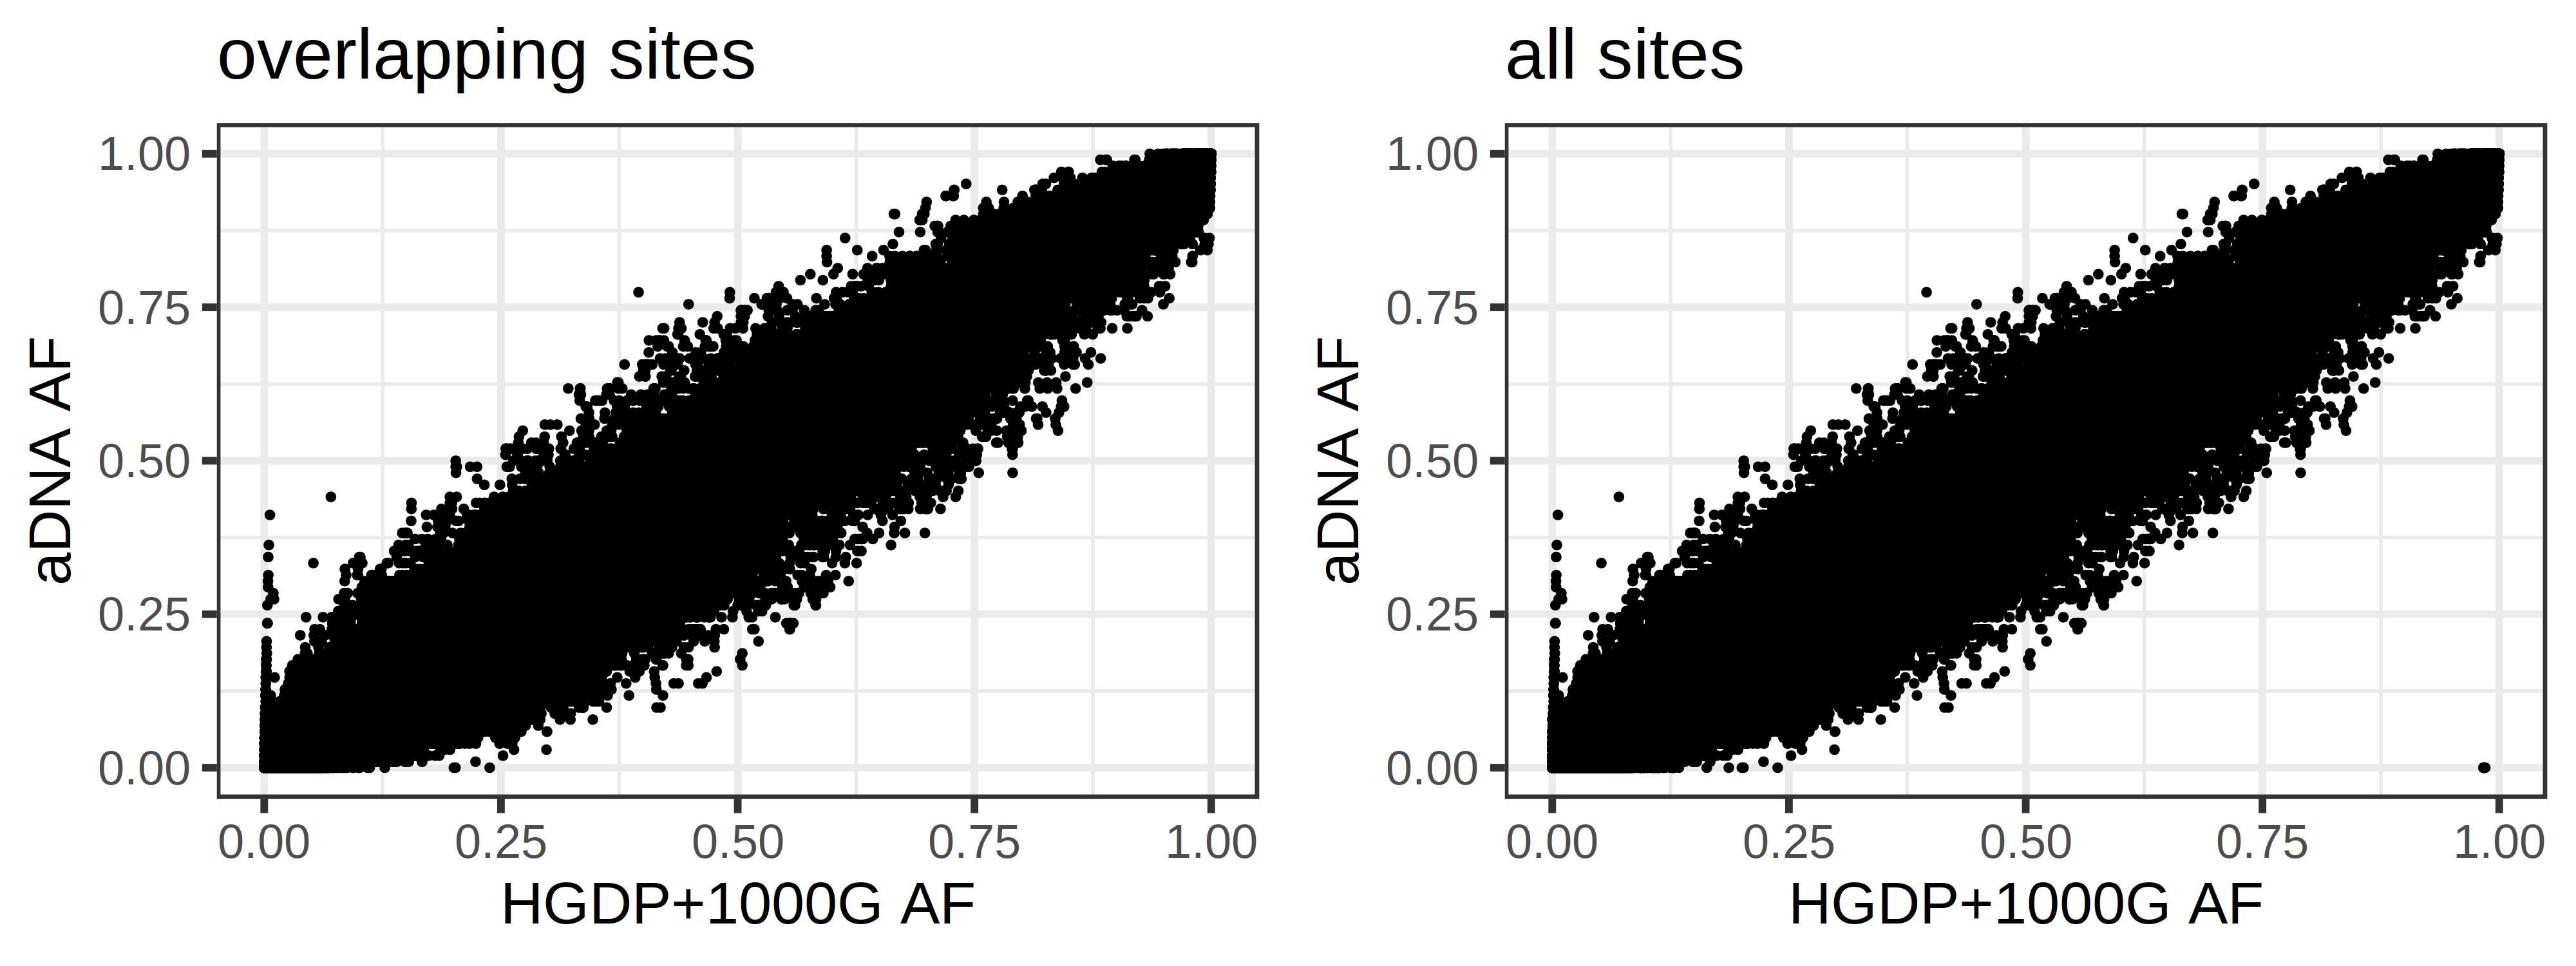
\includegraphics[width=\textwidth]{figures/gb_merge_sanity_check.png}
    \caption{\textbf{Comparison of allele frequencies between HGDP+1000GP and ancient samples.} We analyze biallelic SNPs on chromosome 20 within the masked regions. The comparison includes union (``all sites'') and intersection (``overlapping sites'') of SNPs in the two datasets seperately.}
    \label{fig:gb-sanity-check}
\end{figure}

\begin{figure}[h!]
    \centering
    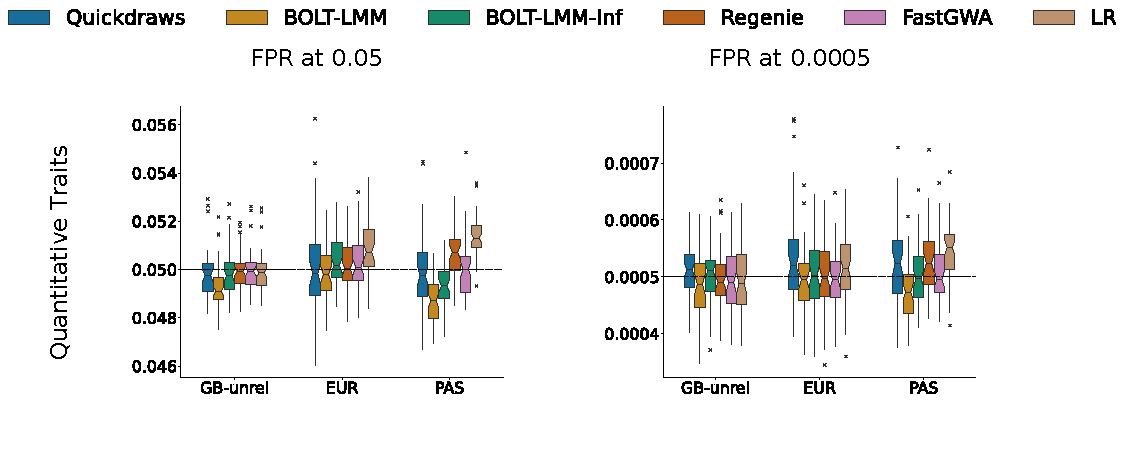
\includegraphics[width=\textwidth]{figures/sim_calibration/popstructure_fpr.pdf}
    \caption{
    \textbf{Summary of calibration in simulations with varying levels of population structure.}
    %
    False positive rate (FPR) at a significance threshold of $\alpha \in \{0.05, 0.0005\}$, calculated as the fraction of variants on even chromosomes with p-value lower than $\alpha$.
    %
    The line inside each box indicates the median value, the central box indicates the interquartile range, whiskers indicate data up to $1.5$ times the IQR, and outliers are shown as separate points.
    %
    A description of the group labels (GB-unrel, EUR, PAS) is provided in section \ref{sec:ch5-sim-design}.
    }
    \label{fig:sim_calib_pop}
\end{figure}

\newpage

\begin{figure}[h!]
    \centering
    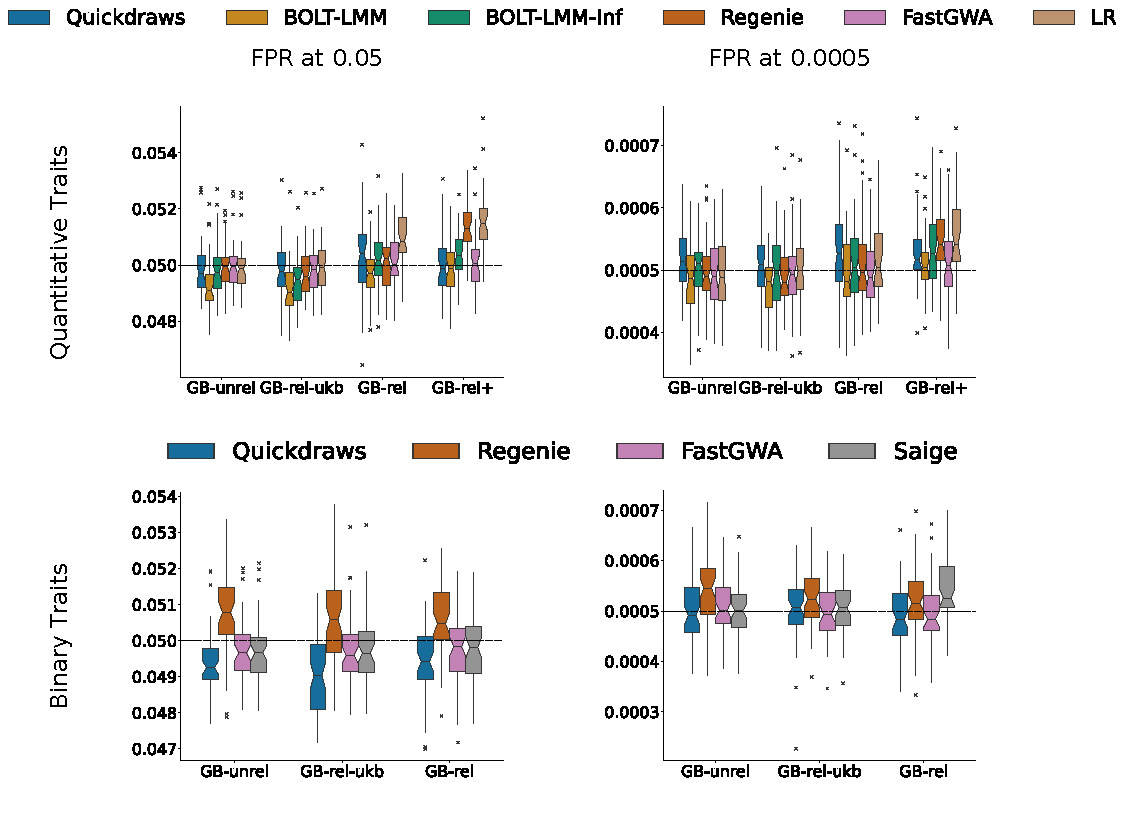
\includegraphics[width=\textwidth]{figures/sim_calibration/relatedness_fpr.pdf}
    \caption{\textbf{Summary of calibration in simulations with varying levels of relatedness.}
    %
    False positive rate (FPR) at a significance threshold of $\alpha \in \{0.05, 0.0005\}$, calculated as the number of variants on even chromosomes with p-value lower than $\alpha$.
    %
    The line inside each box indicates the median value, the central box indicates the interquartile range, whiskers indicate data up to $1.5$ times the IQR, and outliers are shown as separate points.
    %
    GB-unrel refers to simulations including only unrelated British individuals, GB-rel-ukb refers to randomly sampling from the related white British subset, GB-rel refers to the default relatedness setting with $3.4 \times$ more relative pairs compared to the UK Biobank, and GB-rel+ refers to the extreme relatedness case of $7.3 \times$ and $4.8 \times$ more first and second degree relative pairs compared to the UK Biobank.
    %
    The prevalence of binary traits was fixed at 10\%.
    }
    \label{fig:sim_calib_rel}
\end{figure}

\begin{figure}[h!]
    \centering
    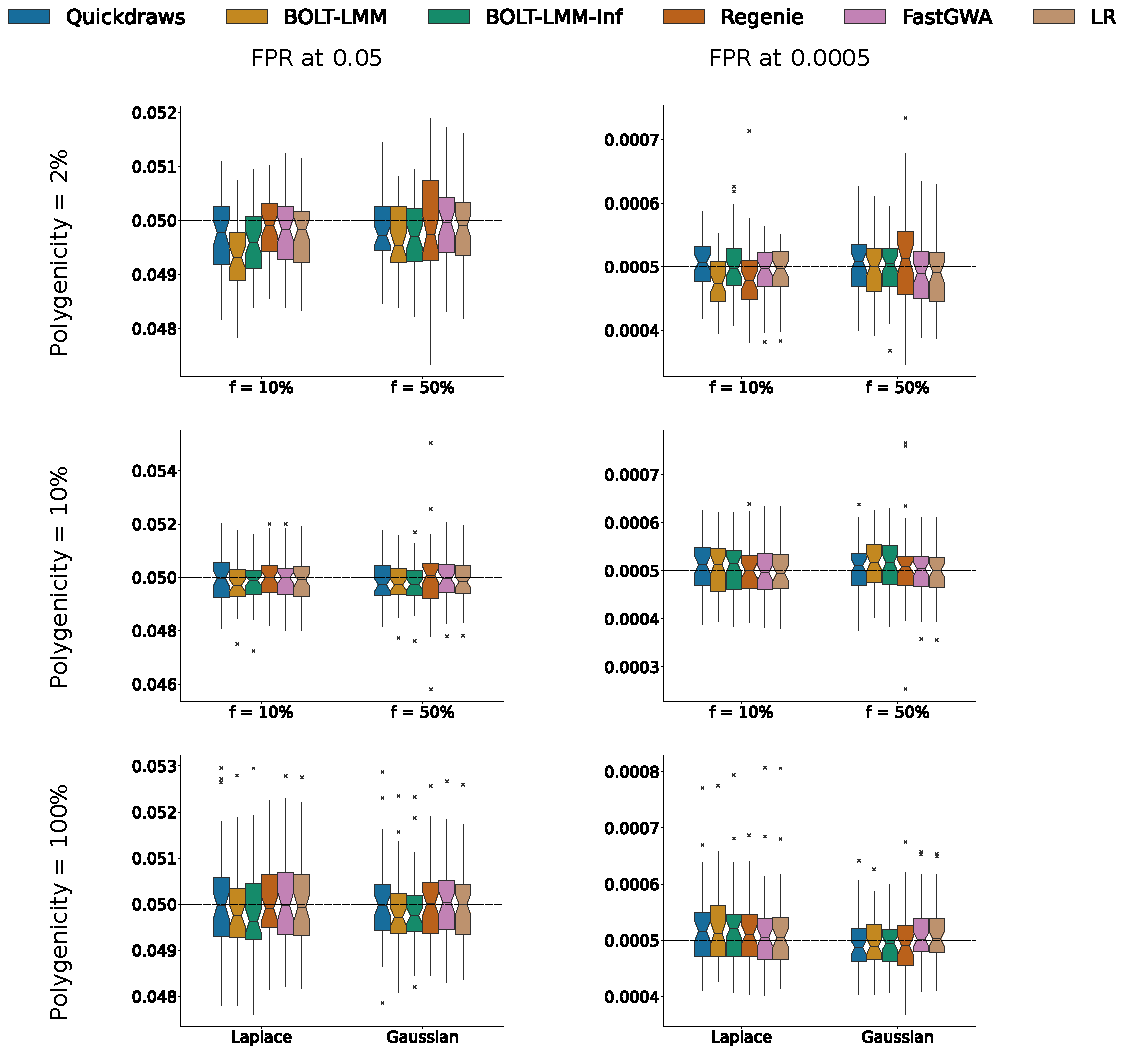
\includegraphics[width=\textwidth]{figures/sim_calibration/mog_fpr.pdf}
    \caption{
    \textbf{Summary of calibration in simulations with varying causal effect distributions.}
    %
    The first two rows correspond to causal effects simulated from a mixture of two Gaussian. 
    %
    Polygenicity refers to the proportion corresponding to the Gaussian with higher variance, and f refers to the fraction of total variance explained by the Gaussian with lower variance.
    %
    False positive rate (FPR) at a significance threshold of $\alpha \in \{0.05, 0.0005\}$, calculated as the fraction of variants on even chromosomes with p-value lower than $\alpha$.
    %
    The line inside each box indicates the median value, the central box indicates the interquartile (IQR) range, whiskers indicate data up to $1.5$ times the IQR, and outliers are shown as separate points.
    %
    \label{fig:sim_calib_mog}
    }
\end{figure}

\begin{figure}[h!]
    \centering
    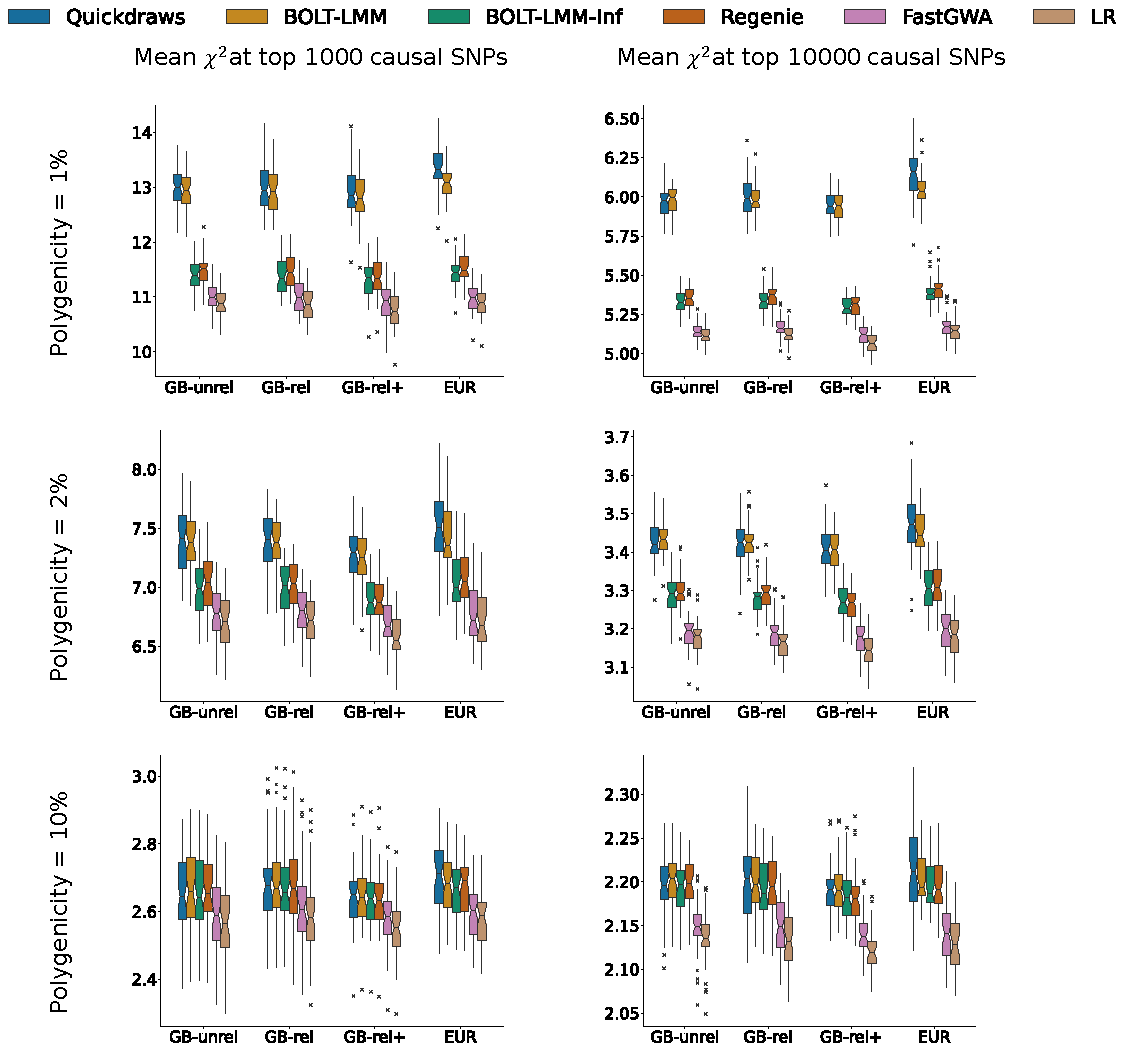
\includegraphics[width=\textwidth]{figures/sim_power/qt_power.pdf}
    
    \caption{\textbf{Summary of statistical power in simulations for quantitative traits.}
    %
    We measure the normalized causal $\chi^2$ at top $1{,}000$ and top $10{,}000$ causal variants.
    %
    To correct for confounding, the causal $\chi^2$ is normalized by the average $\chi^2$ at null variants on even chromosomes.
    %
    The line inside each box indicates the median value, the central box indicates the interquartile range, whiskers indicate data up to $1.5$ times the IQR, and outliers are shown as separate points.
    %
    A description of the group labels (GB-unrel, GB-rel, GB-rel+, EUR) is provided in section \ref{sec:ch5-sim-design}.
    \label{fig:sim_power_qt}
    }
\end{figure}

\begin{figure}[h!]
    \centering
    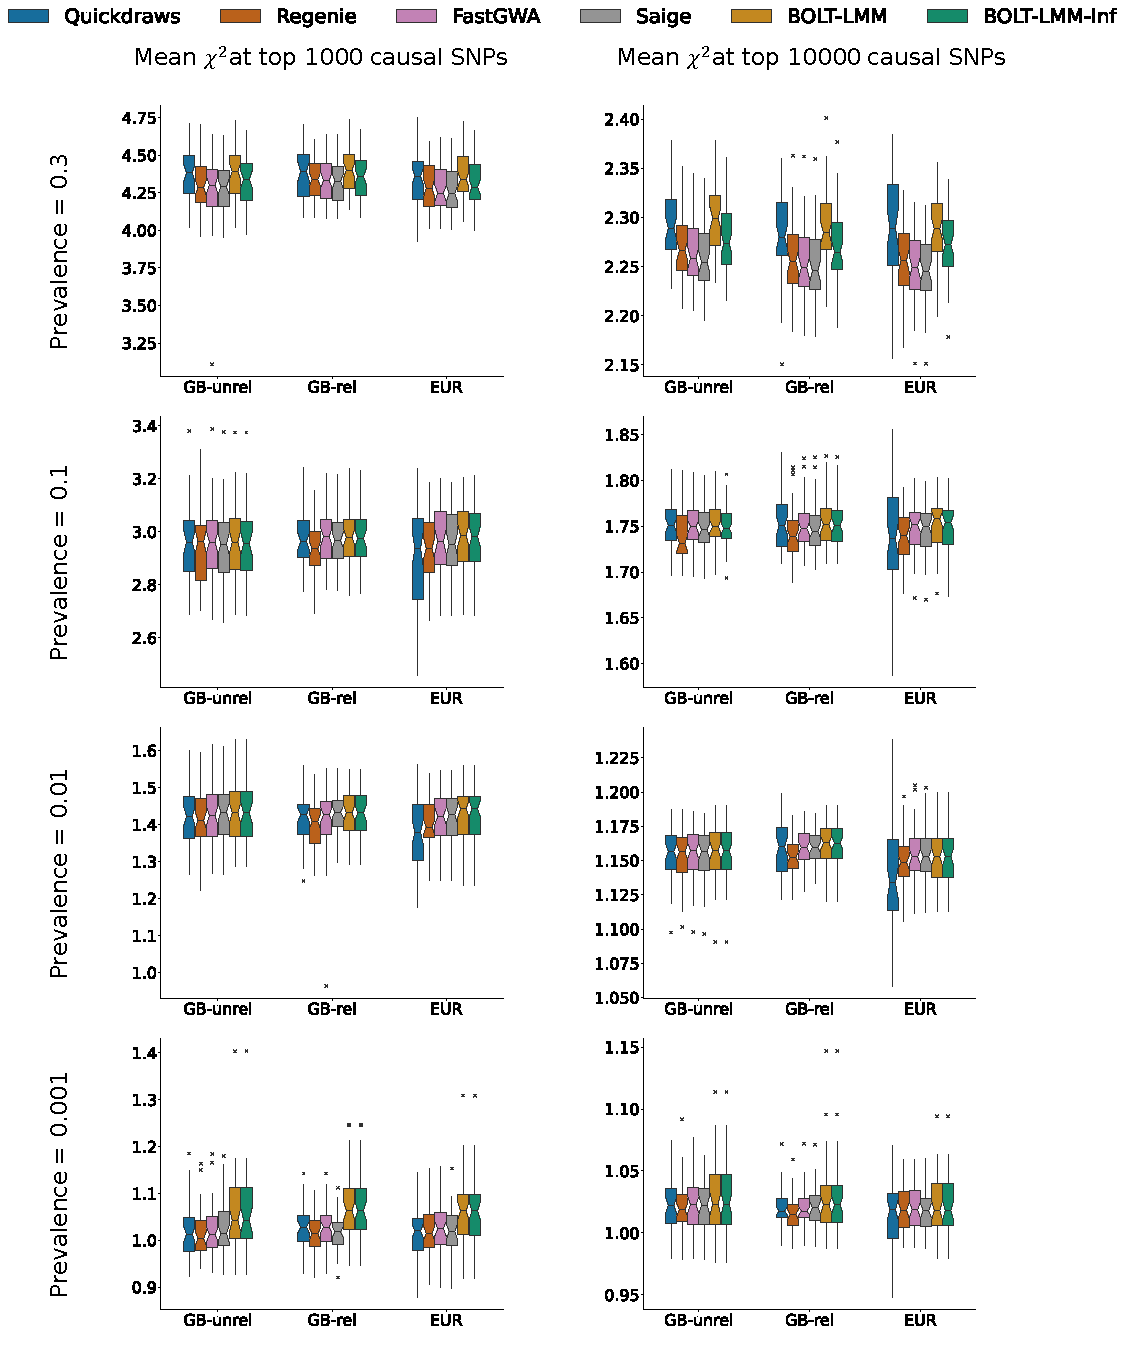
\includegraphics[width=\textwidth]{figures/sim_power/bt_power.pdf}
    
    \caption{\textbf{Summary of statistical power in simulations for binary traits.}
    %
    We measure the normalized causal $\chi^2$ at top $1{,}000$ and top $10{,}000$ causal variants.
    %
    To correct for confounding, the causal $\chi^2$ is normalized by the average $\chi^2$ at null variants on even chromosomes.
    %
    The line inside each box indicates the median value, the central box indicates the interquartile range, whiskers indicate data up to $1.5$ times the IQR, and outliers are shown as separate points.
    %
    A description of the group labels (GB-unrel, GB-rel, EUR) is provided in the section \ref{sec:ch5-sim-design}.
    \label{fig:sim_power_bt}
    }
\end{figure}

\begin{figure}[h!]
    \centering
    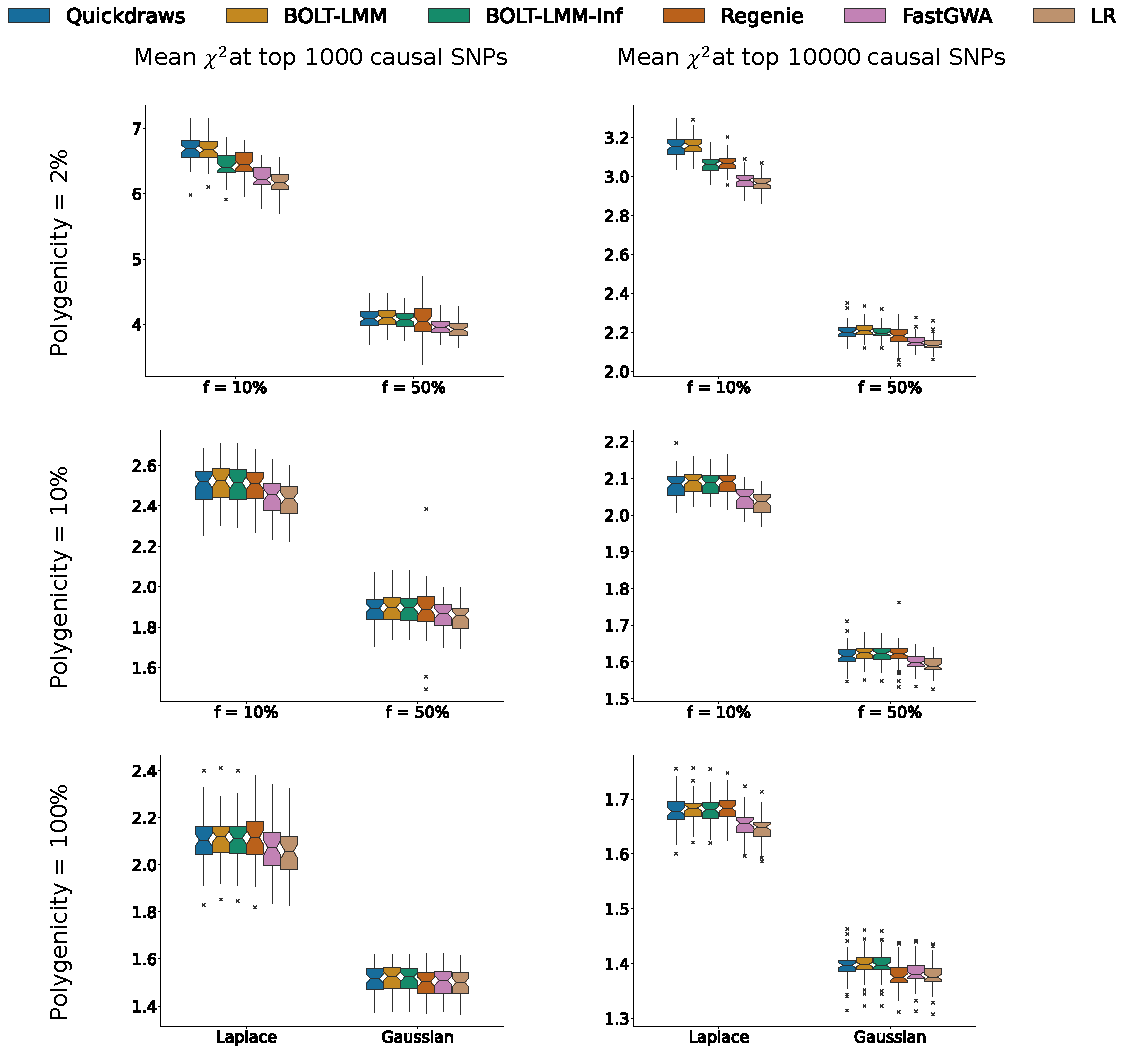
\includegraphics[width=\textwidth]{figures/sim_power/mog_power.pdf}
    \caption{
    \textbf{Summary of statistical power in simulations with varying causal effect distributions.}
    %
    The first two rows correspond to causal effects simulated from a mixture of two Gaussian. 
    %
    Polygenicity refers the proportion corresponding to the Gaussian with higher variance, and f refers to the fraction of total variance explained by the Gaussian with lower variance.
    %
    We measure the normalized causal $\chi^2$ at top $1{,}000$ and top $10{,}000$ causal variants.
    %
    To correct for confounding, the causal $\chi^2$ is normalized by the average $\chi^2$ at null variants on even chromosomes.
    %
    The line inside each box indicates the median value, the central box indicates the interquartile range (IQR), whiskers indicate data up to $1.5$ times the IQR, and outliers are shown as separate points.
    }
    %
    \label{fig:sim_power_mog}
\end{figure}

\begin{figure}[h!]
    \centering
    
\includegraphics[scale=0.425]{figures/manhattan_bin/legend.png}
    \begin{subfigure}{.5\textwidth}
    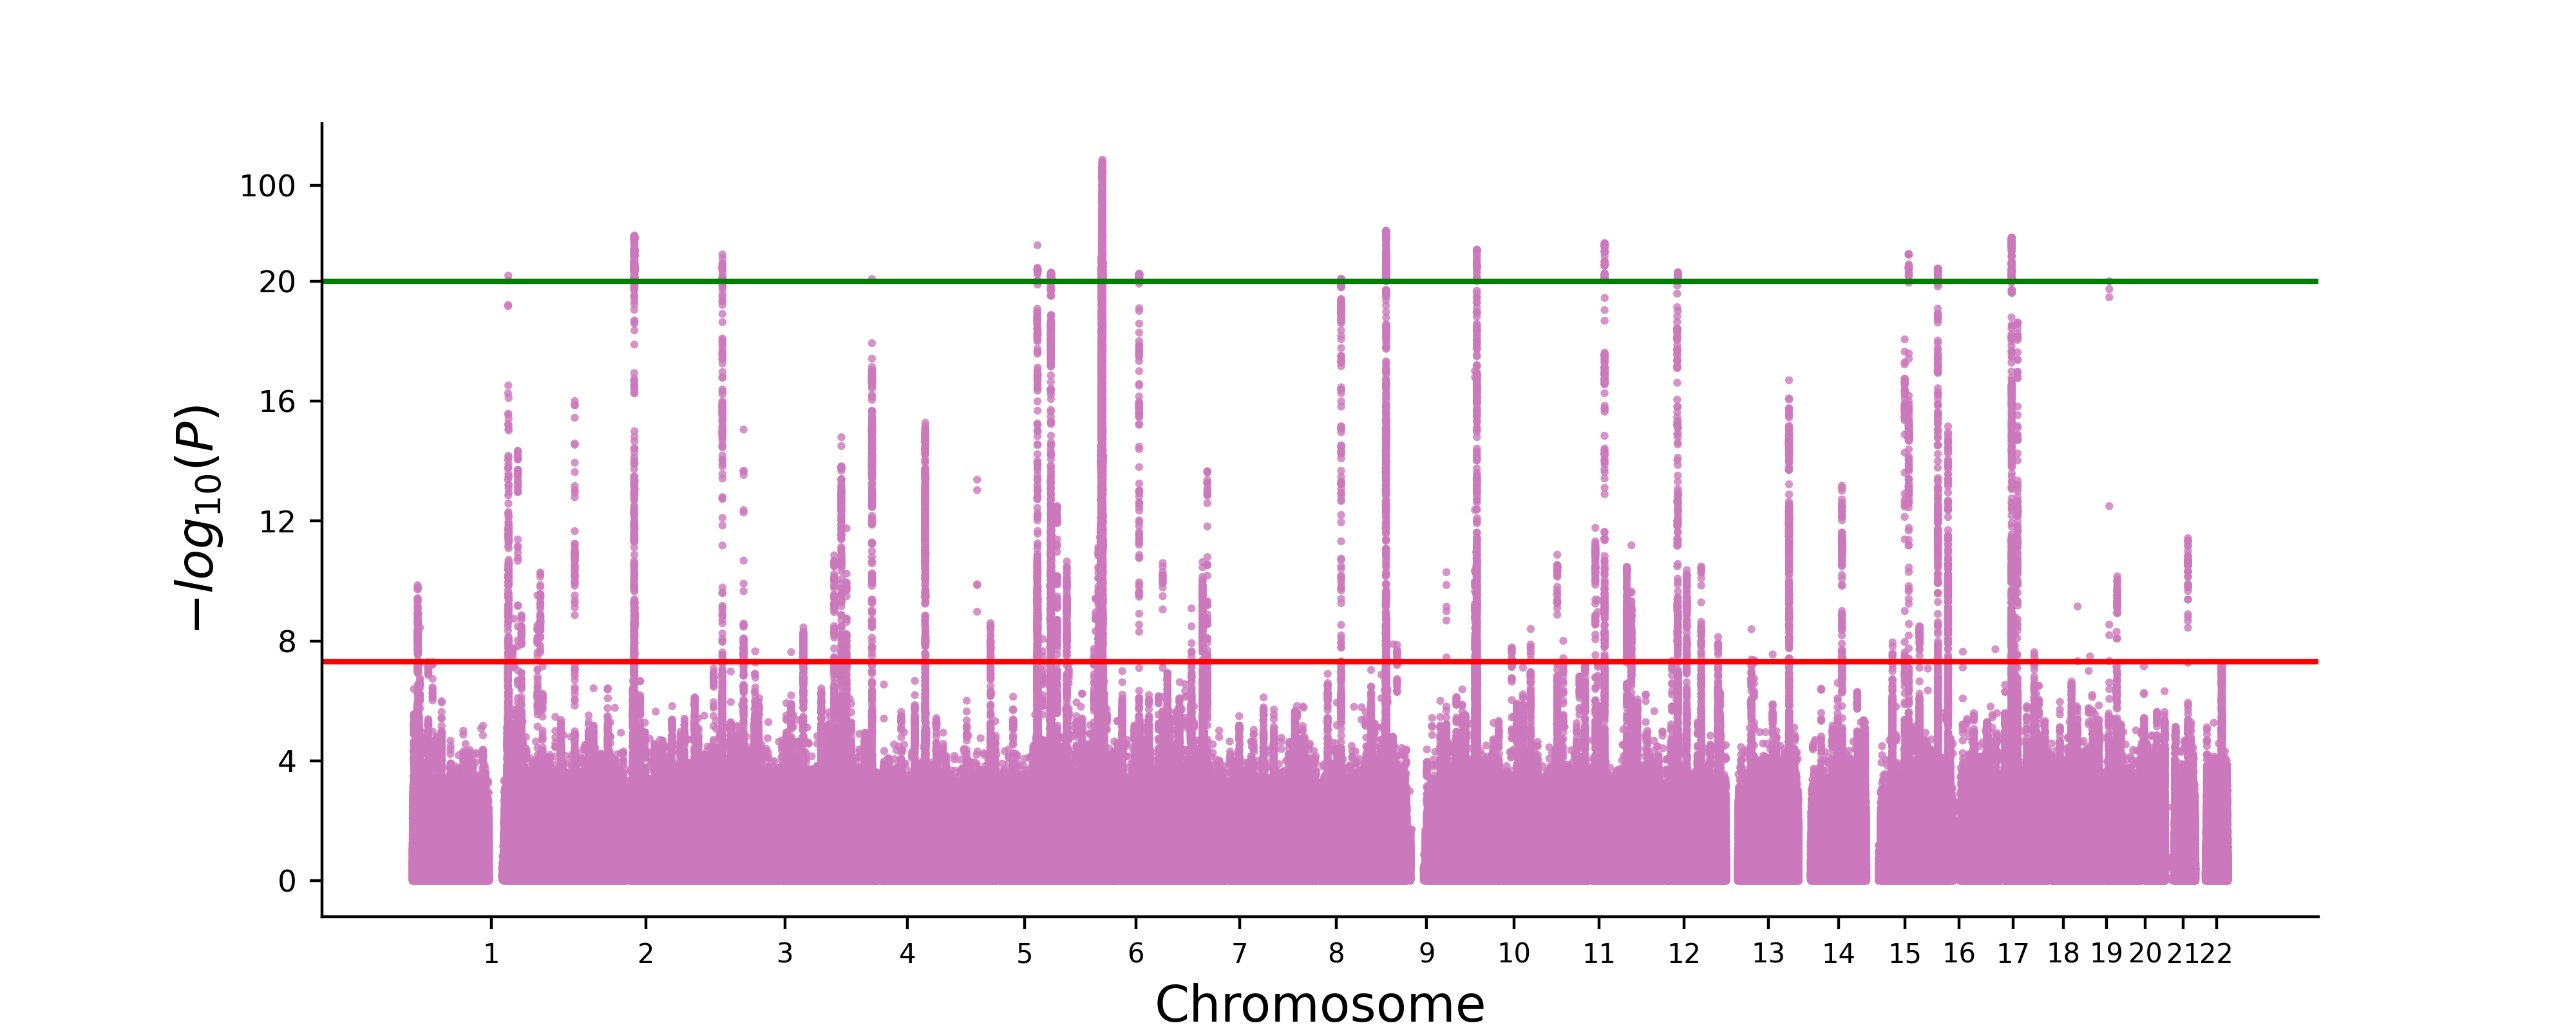
\includegraphics[width=\textwidth]{figures/manhattan_bin/fastgwa_400k1.png}
    \end{subfigure}%
    \begin{subfigure}{.5\textwidth}
    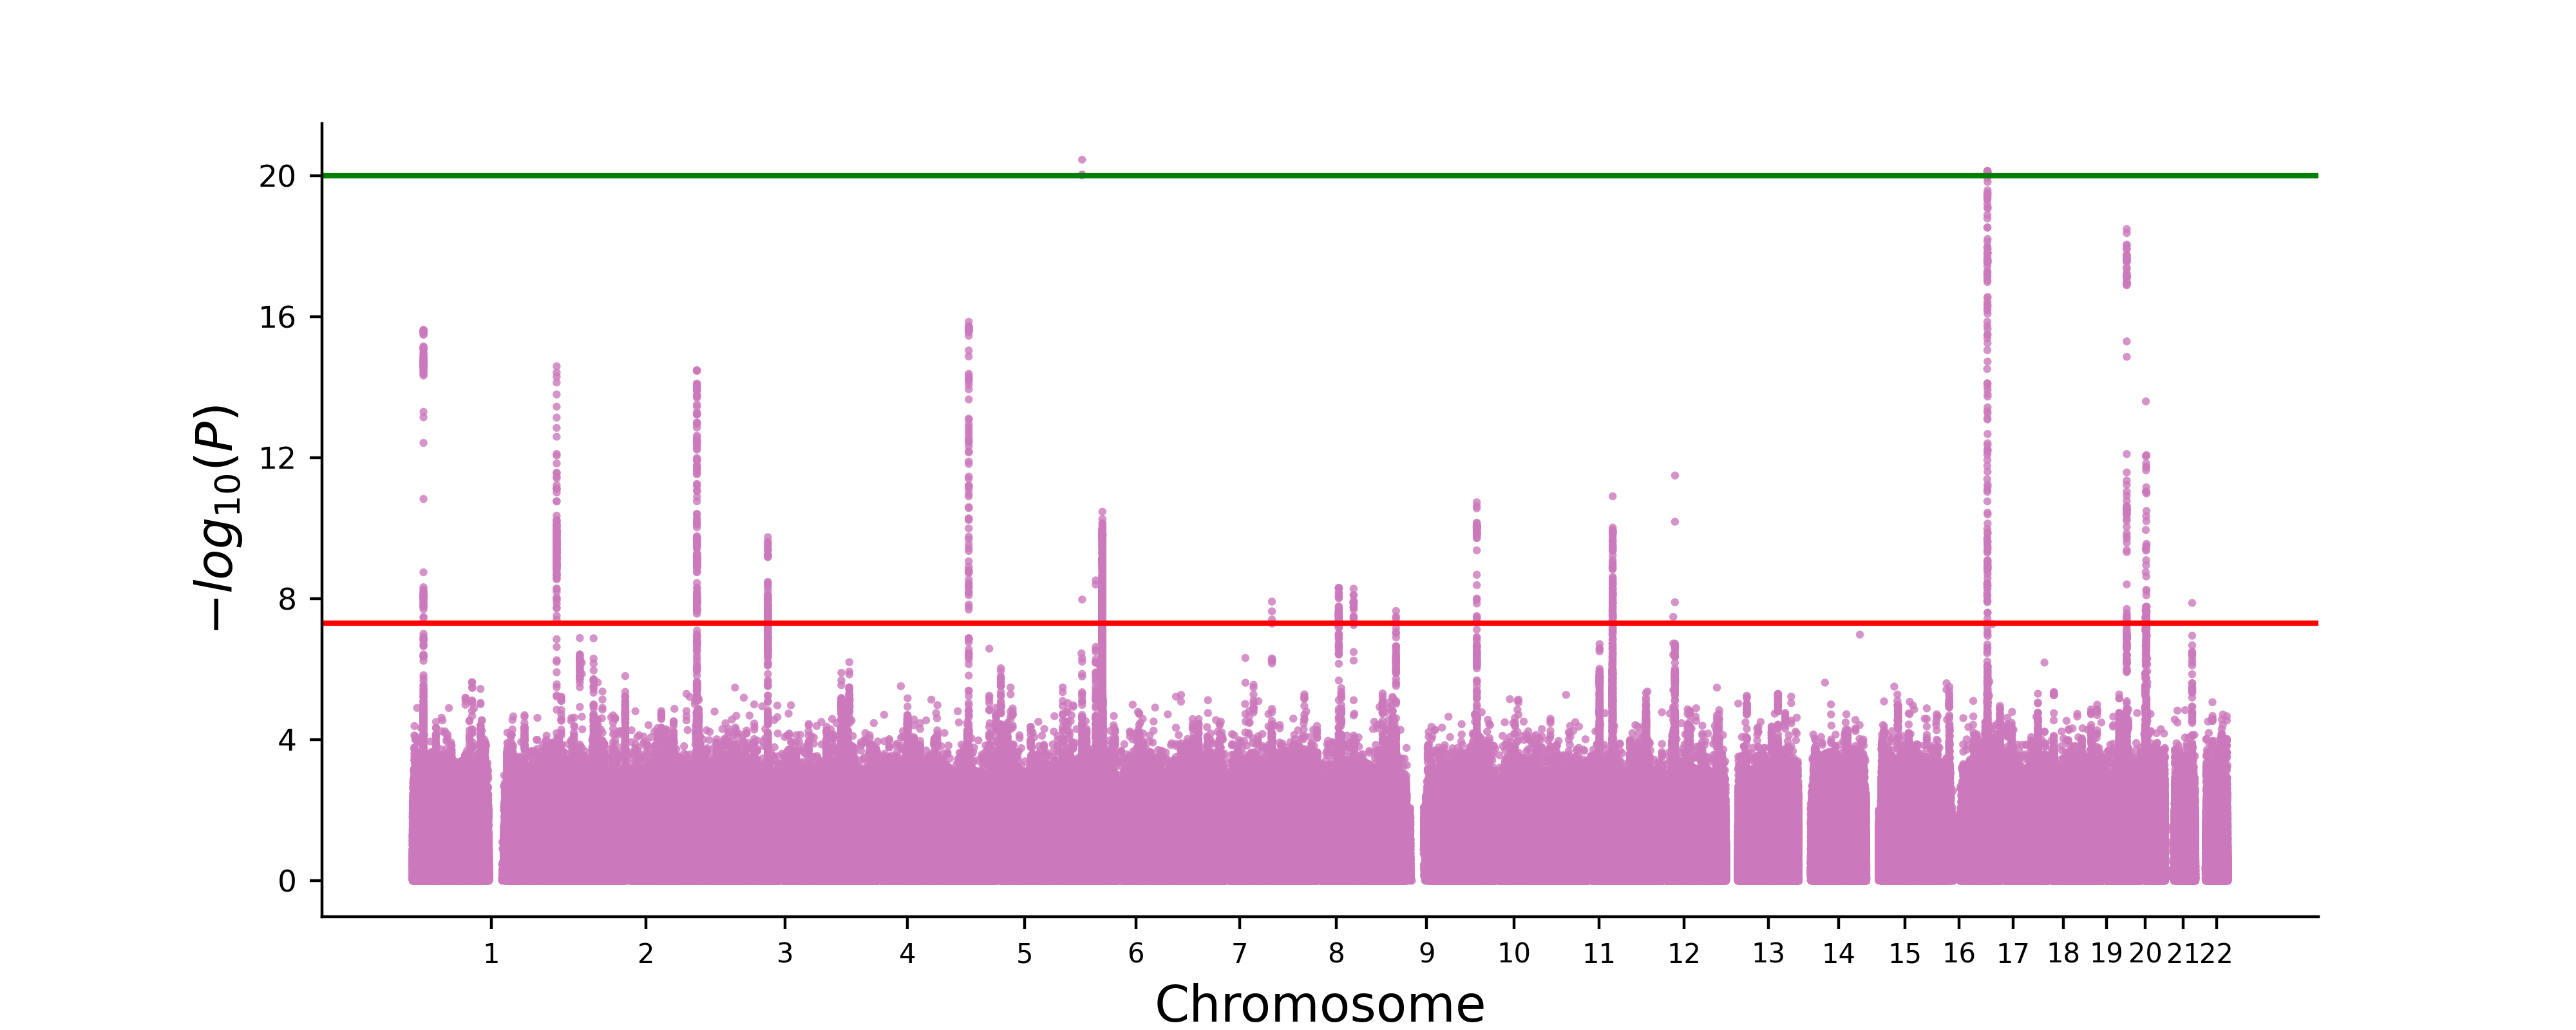
\includegraphics[width=\textwidth]{figures/manhattan_bin/fastgwa_400k16.png}
    \end{subfigure}
    \begin{subfigure}{.5\textwidth}
    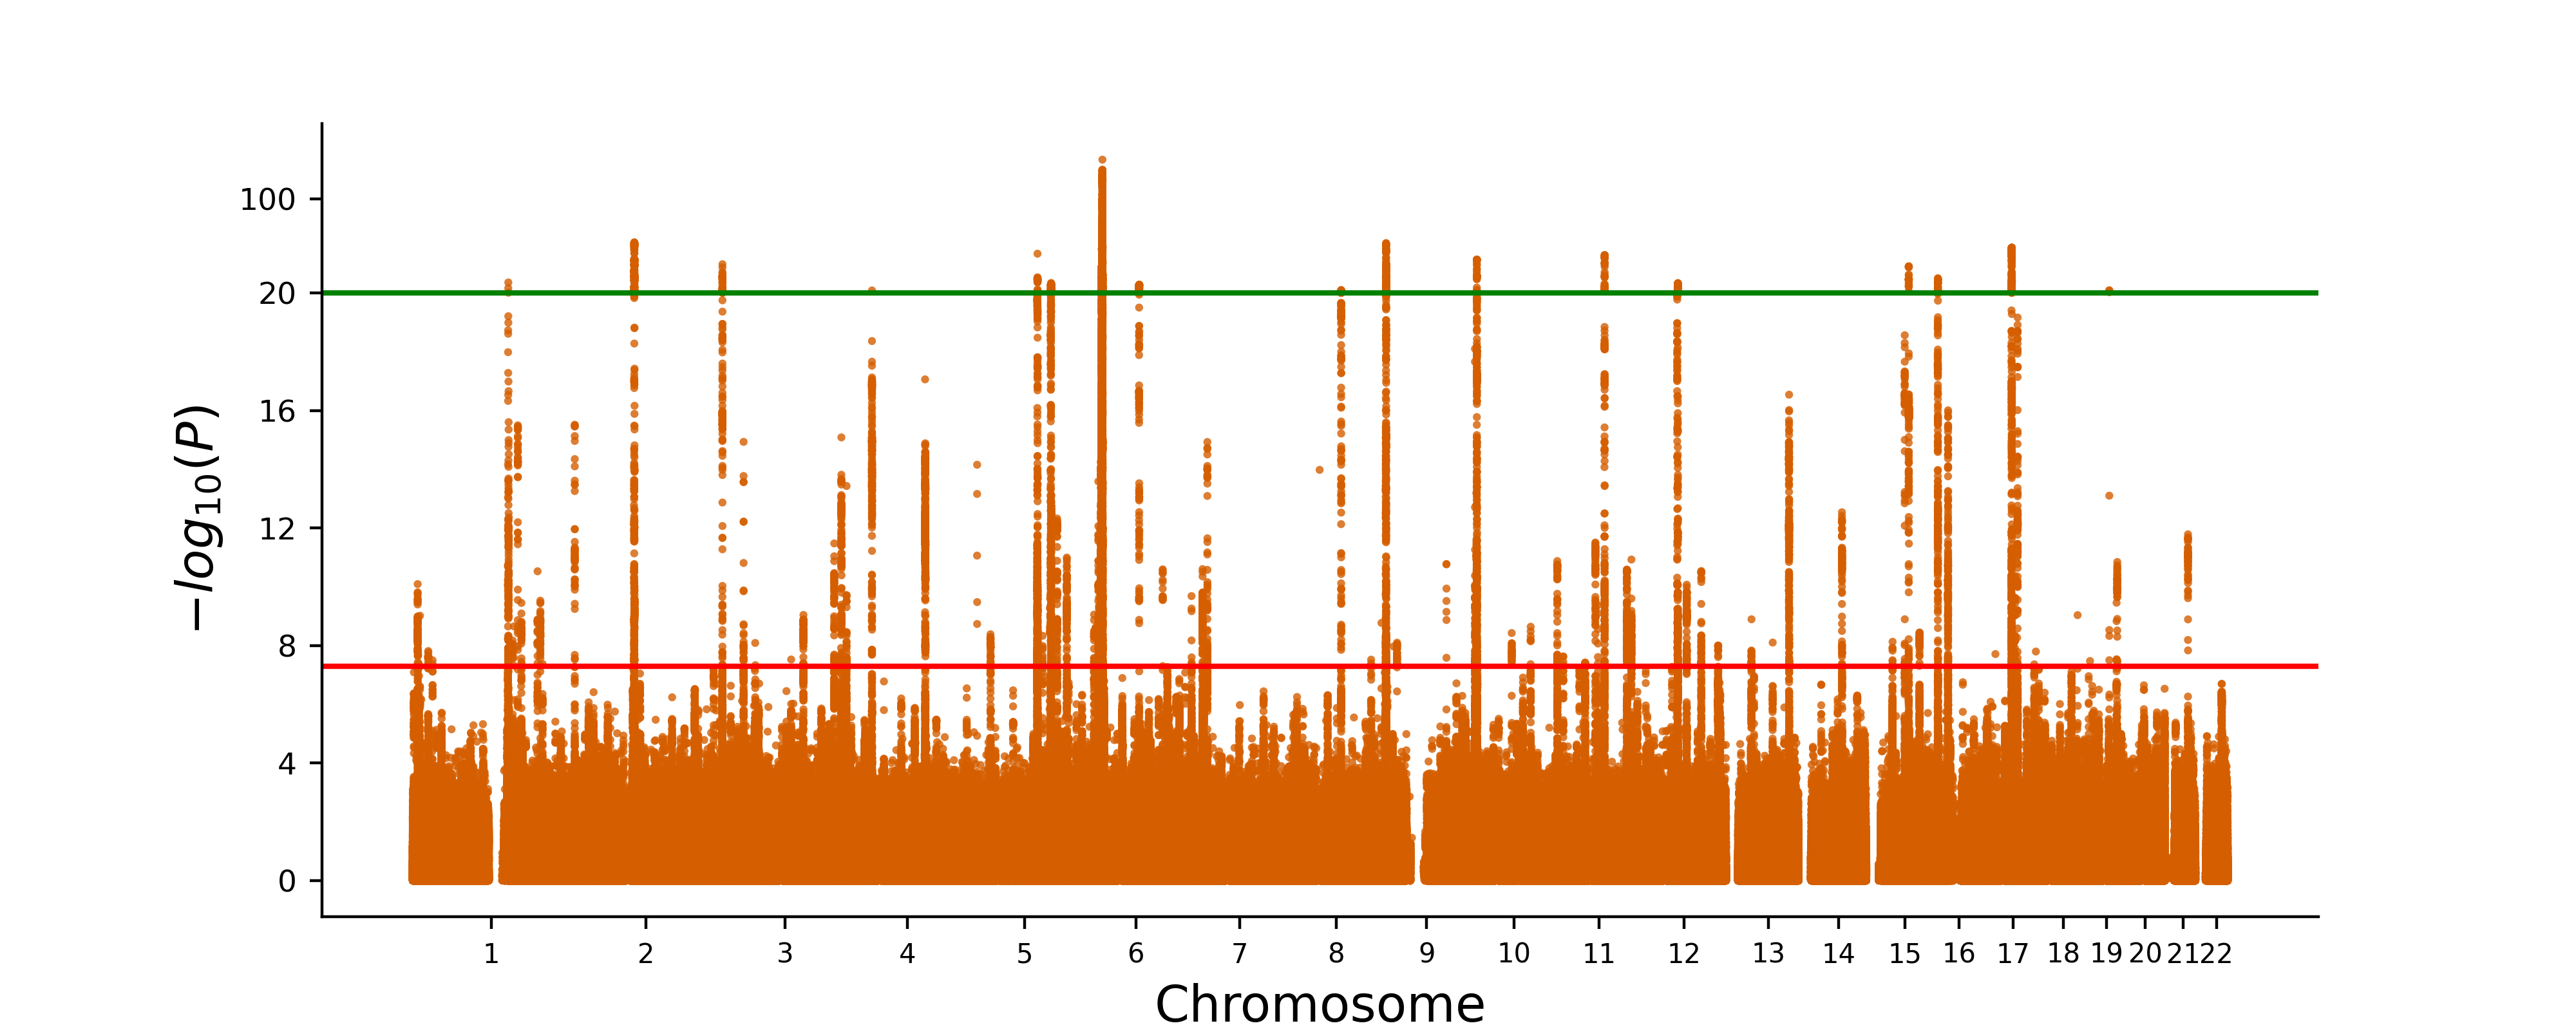
\includegraphics[width=\textwidth]{figures/manhattan_bin/regenie_400kAsthma.png}
    \end{subfigure}%
    \begin{subfigure}{.5\textwidth}
    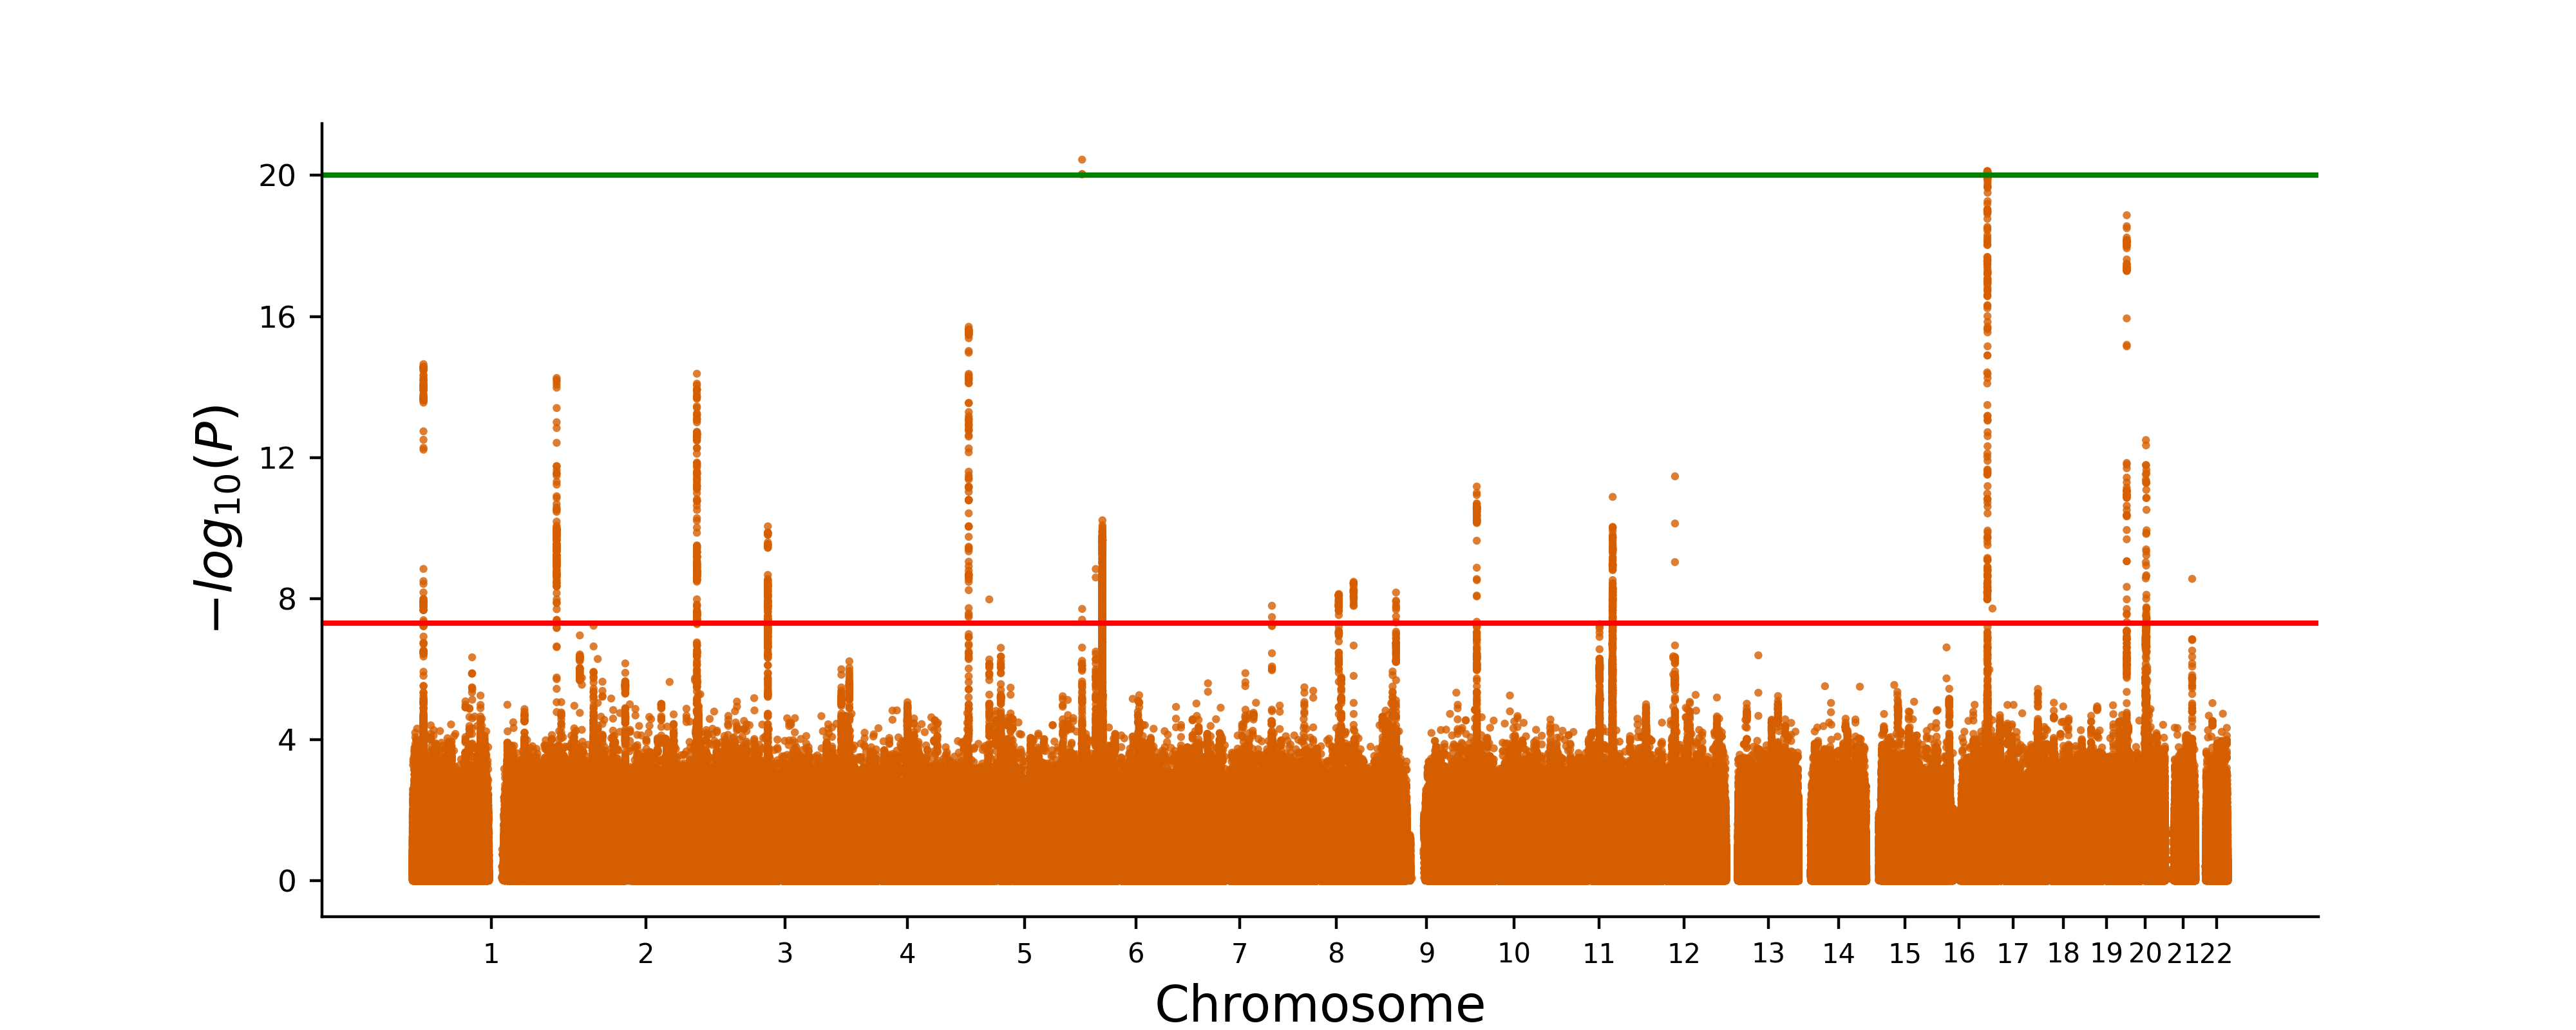
\includegraphics[width=\textwidth]{figures/manhattan_bin/regenie_400kBasal_cell_carcinoma.png}
    \end{subfigure}
    \begin{subfigure}{.5\textwidth}
    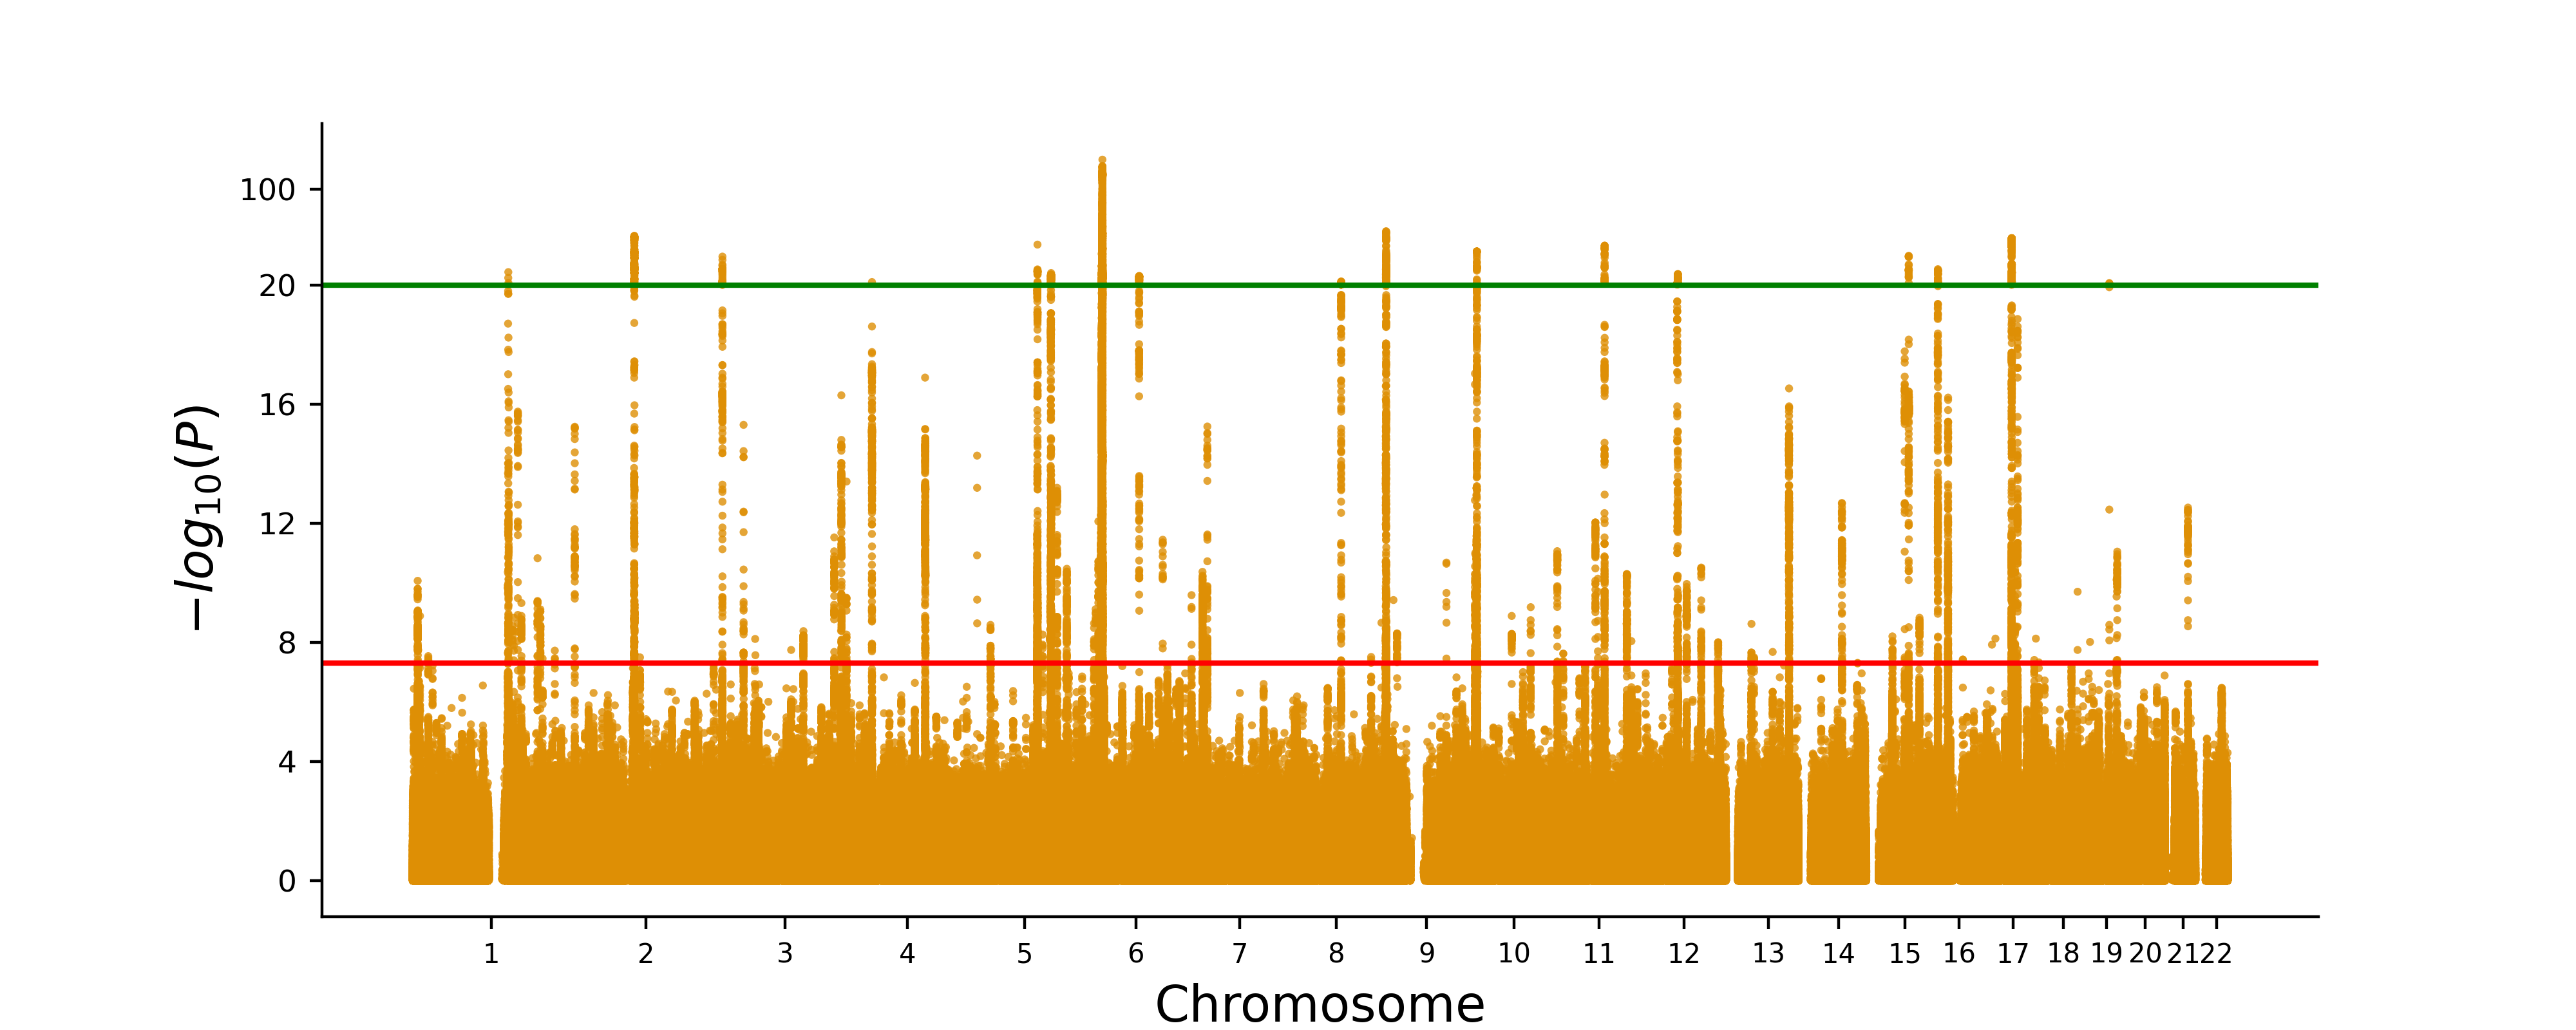
\includegraphics[width=\textwidth]{figures/manhattan_bin/imputed_bgen_bolt_0.sumstats.gz.png}
    \end{subfigure}%
    \begin{subfigure}{.5\textwidth}
    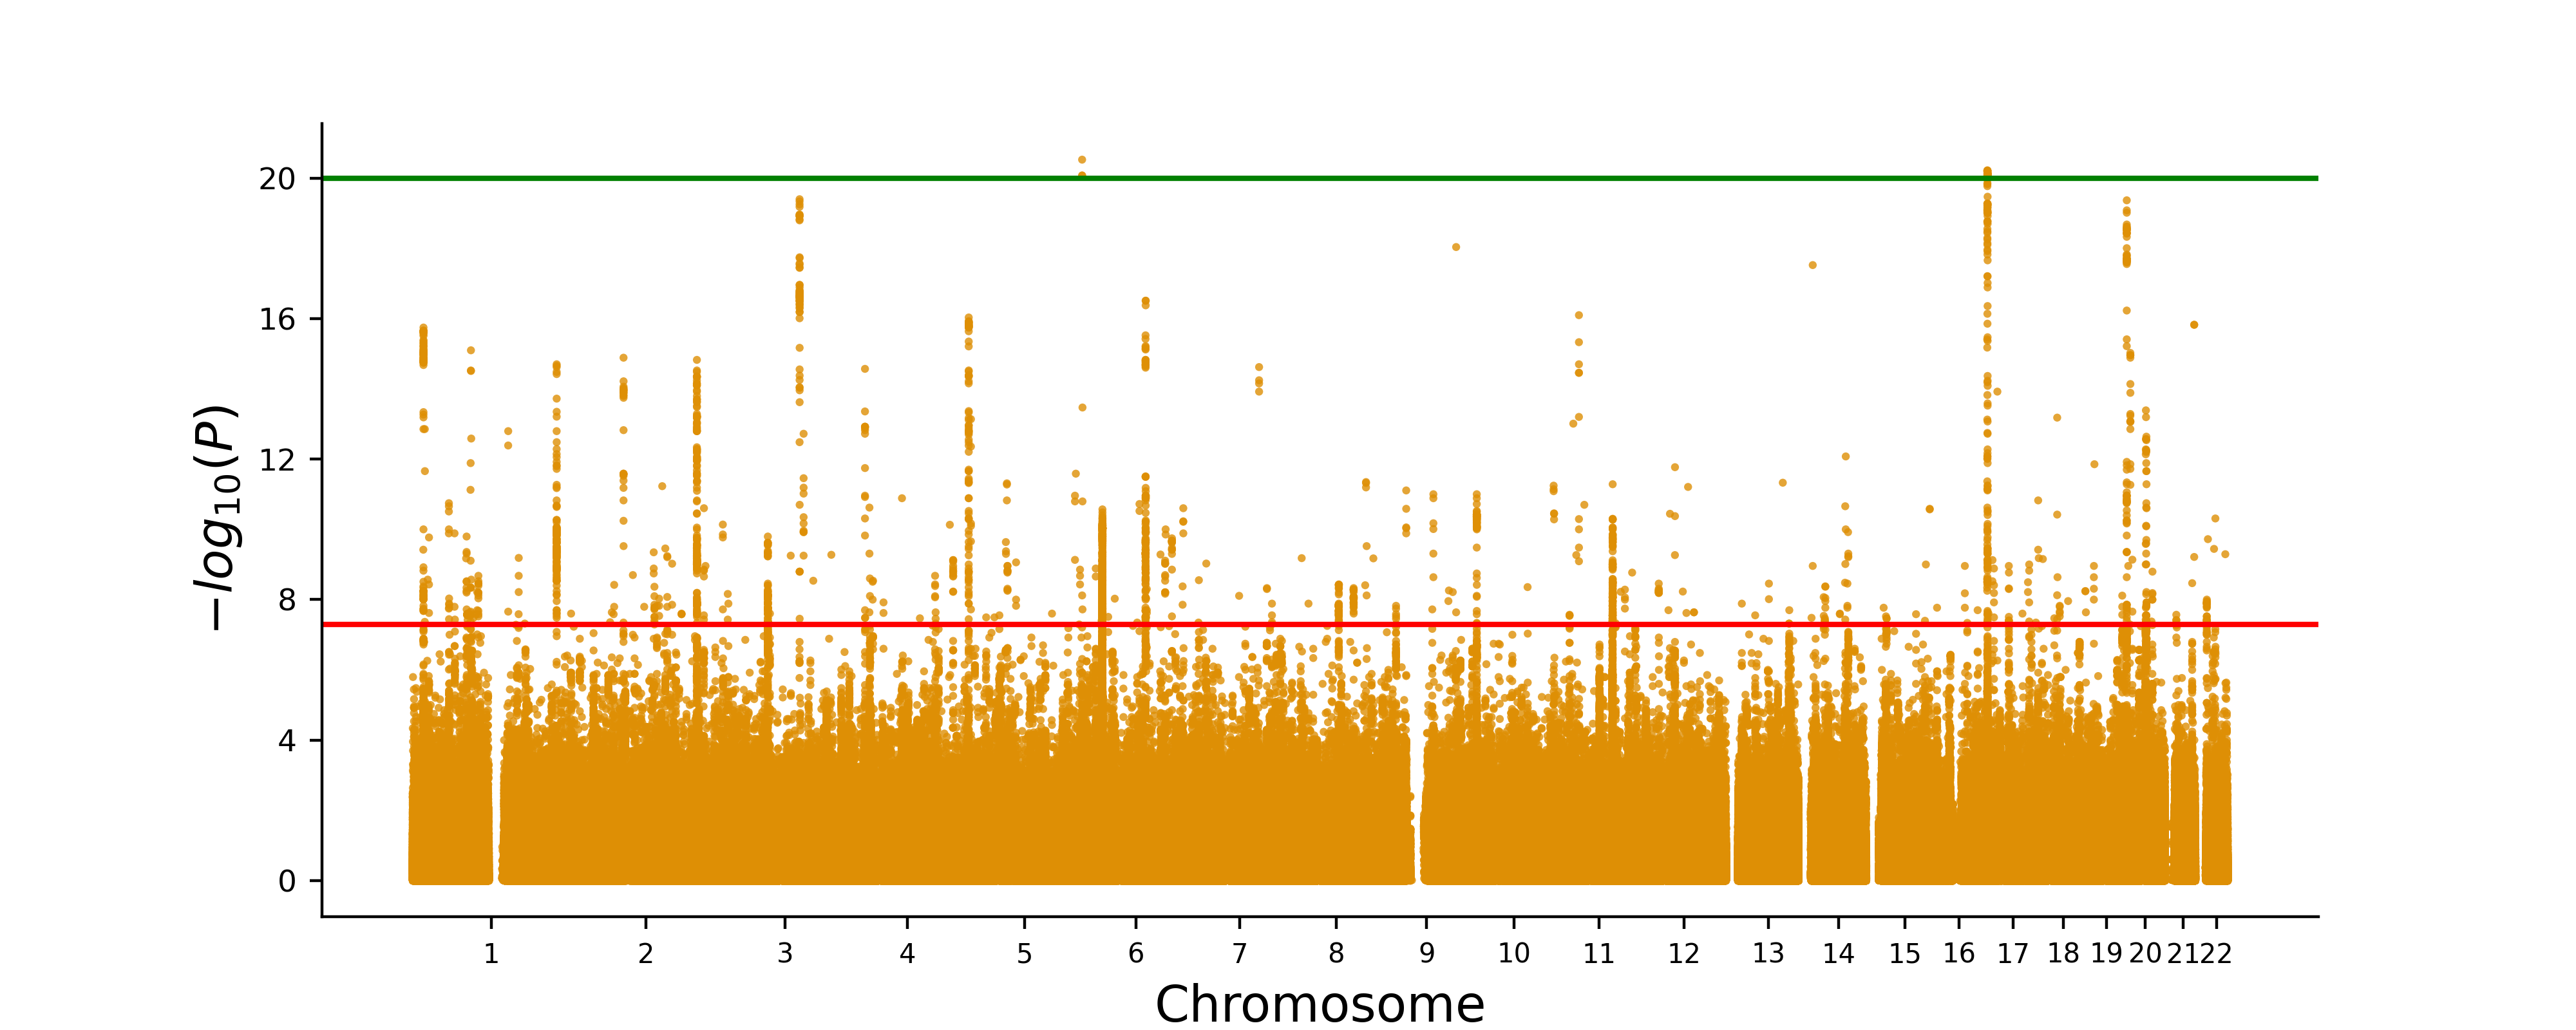
\includegraphics[width=\textwidth]{figures/manhattan_bin/imputed_bgen_bolt_1.sumstats.gz.png}
    \end{subfigure}
    \begin{subfigure}{.5\textwidth}
    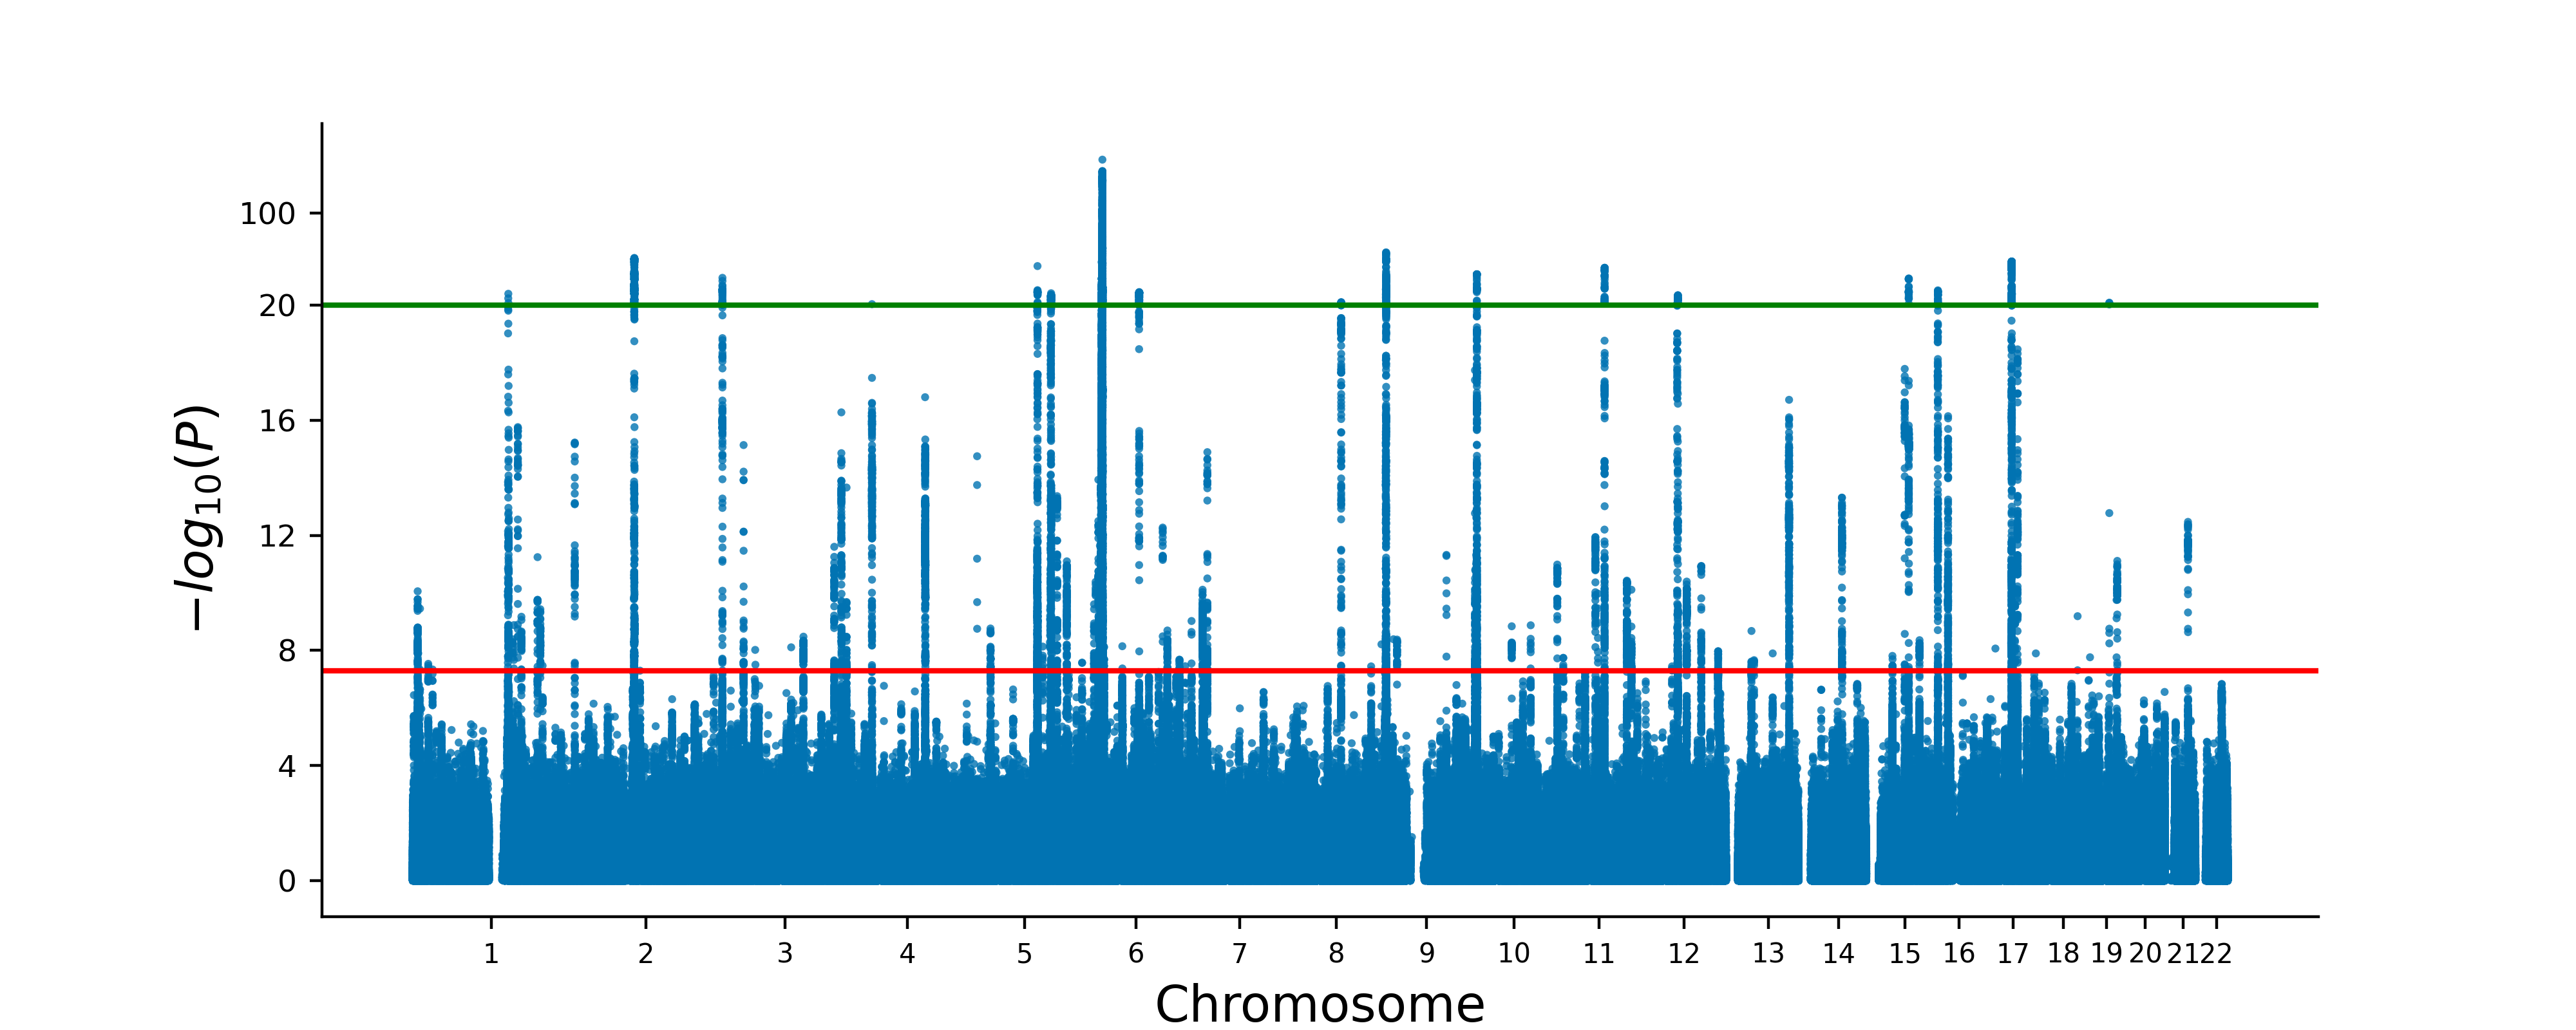
\includegraphics[width=\textwidth]{figures/manhattan_bin/qd_Asthma.sumstats.gz.png}
    \caption{}
    \end{subfigure}%
    \begin{subfigure}{.5\textwidth}
    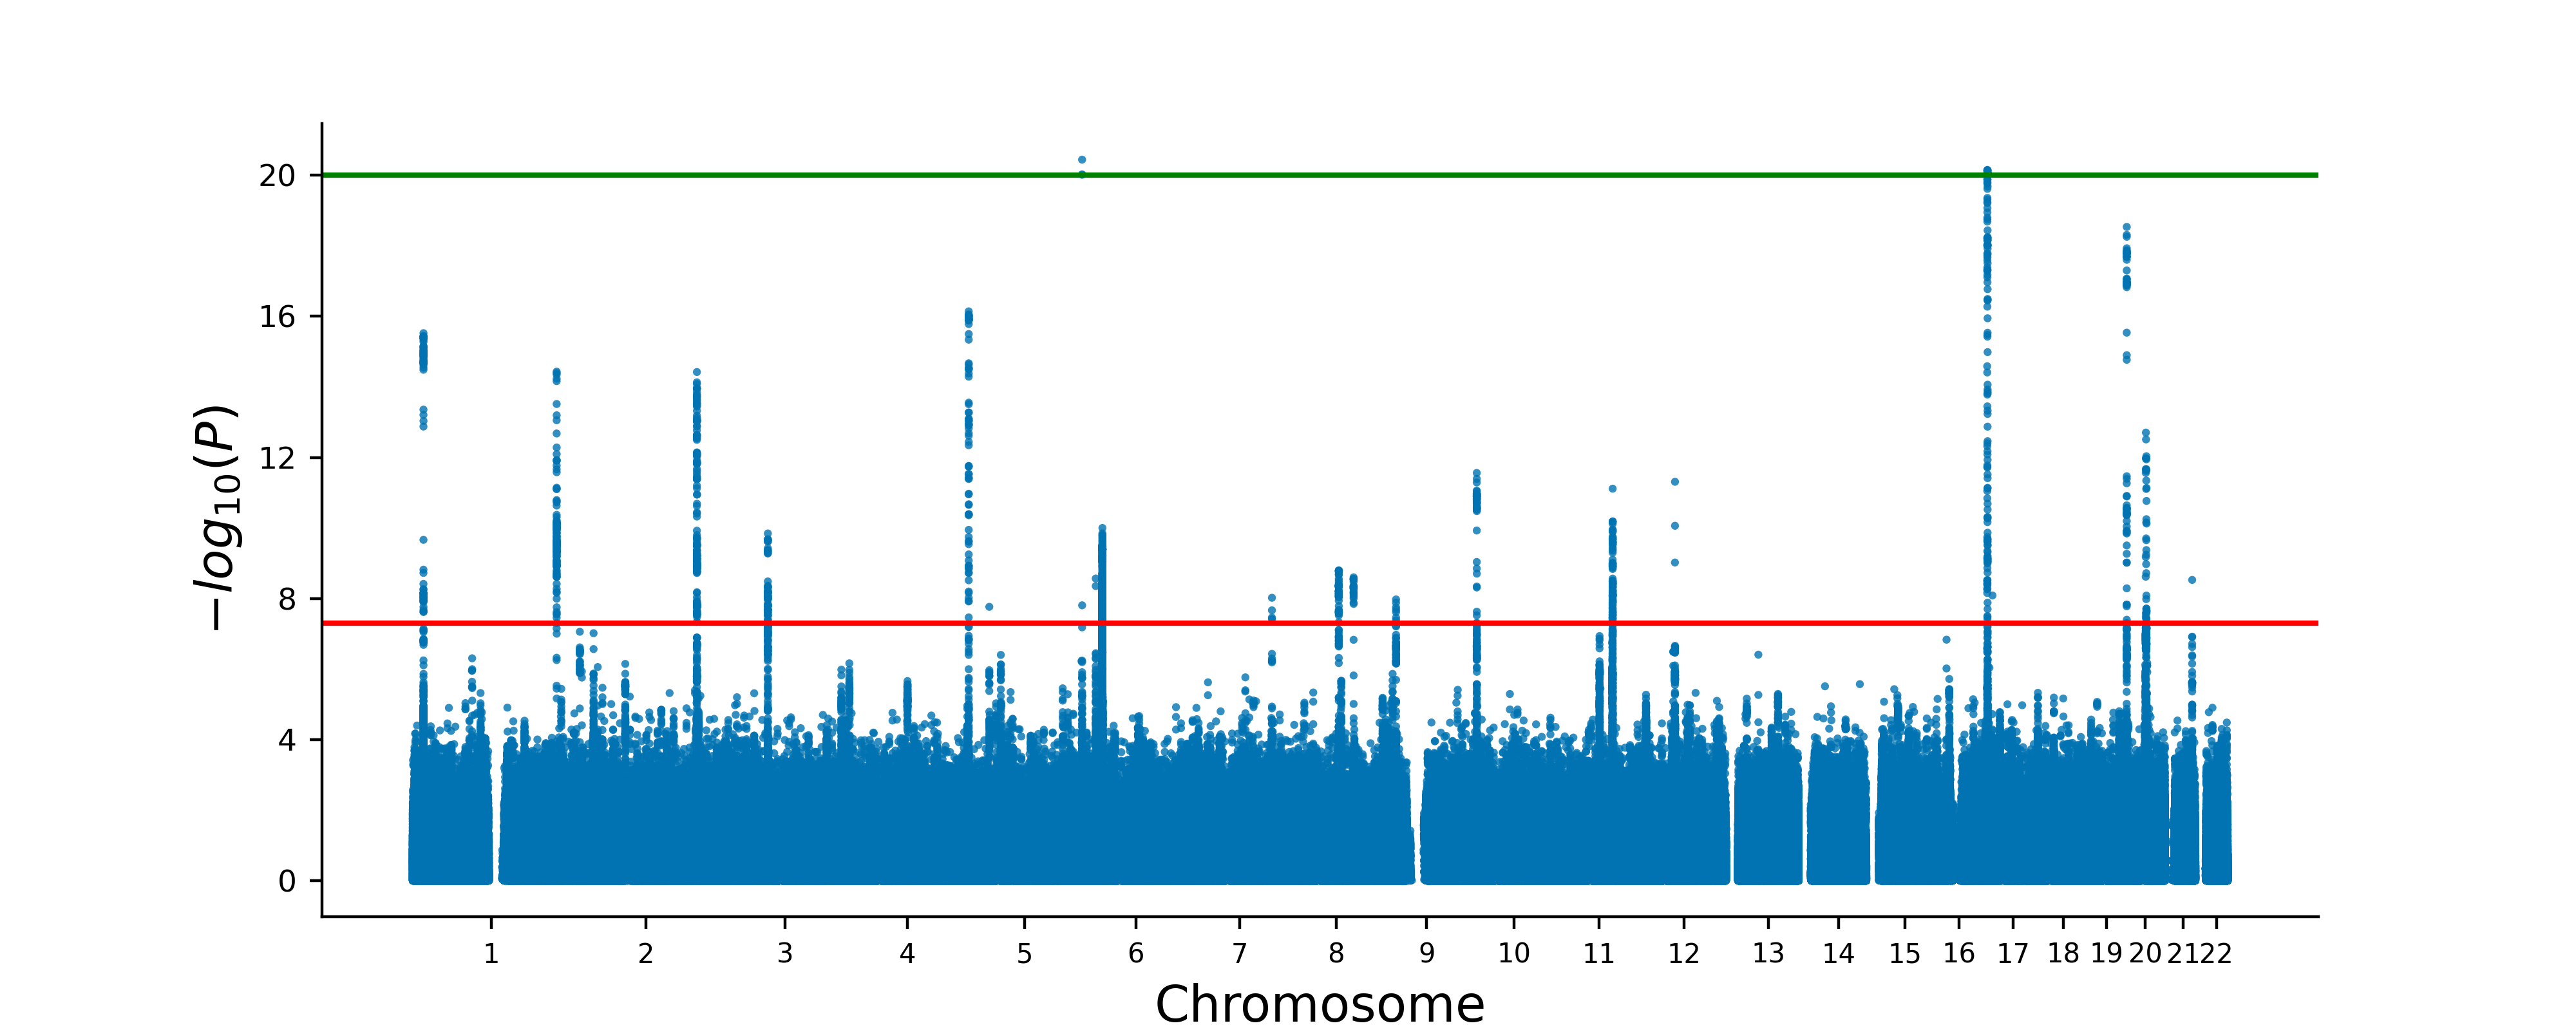
\includegraphics[width=\textwidth]{figures/manhattan_bin/qd_Basal_cell_carcinoma.sumstats.gz.png}
    \caption{}
    \end{subfigure}
    \caption{\textbf{Manhattan plots for two binary traits.}
    %
    (a) Asthma (prevalence $= 0.119$) and (b) Basal cell carcinoma (prevalence $= 0.012$).
    %
    ${\sim}13.3$ million variants were tested.
    %
    Red lines indicate a genome-wide significance threshold of $ P = 5 \times 10^{-8}$ and the green line indicates $P = 1 \times 10^{-20}$.
    }
    \label{fig:qd_man_bin1}
\end{figure}

\begin{figure}[h!]
    \centering
    
\includegraphics[scale=0.425]{figures/manhattan_bin/legend.png}
    \begin{subfigure}{.5\textwidth}
    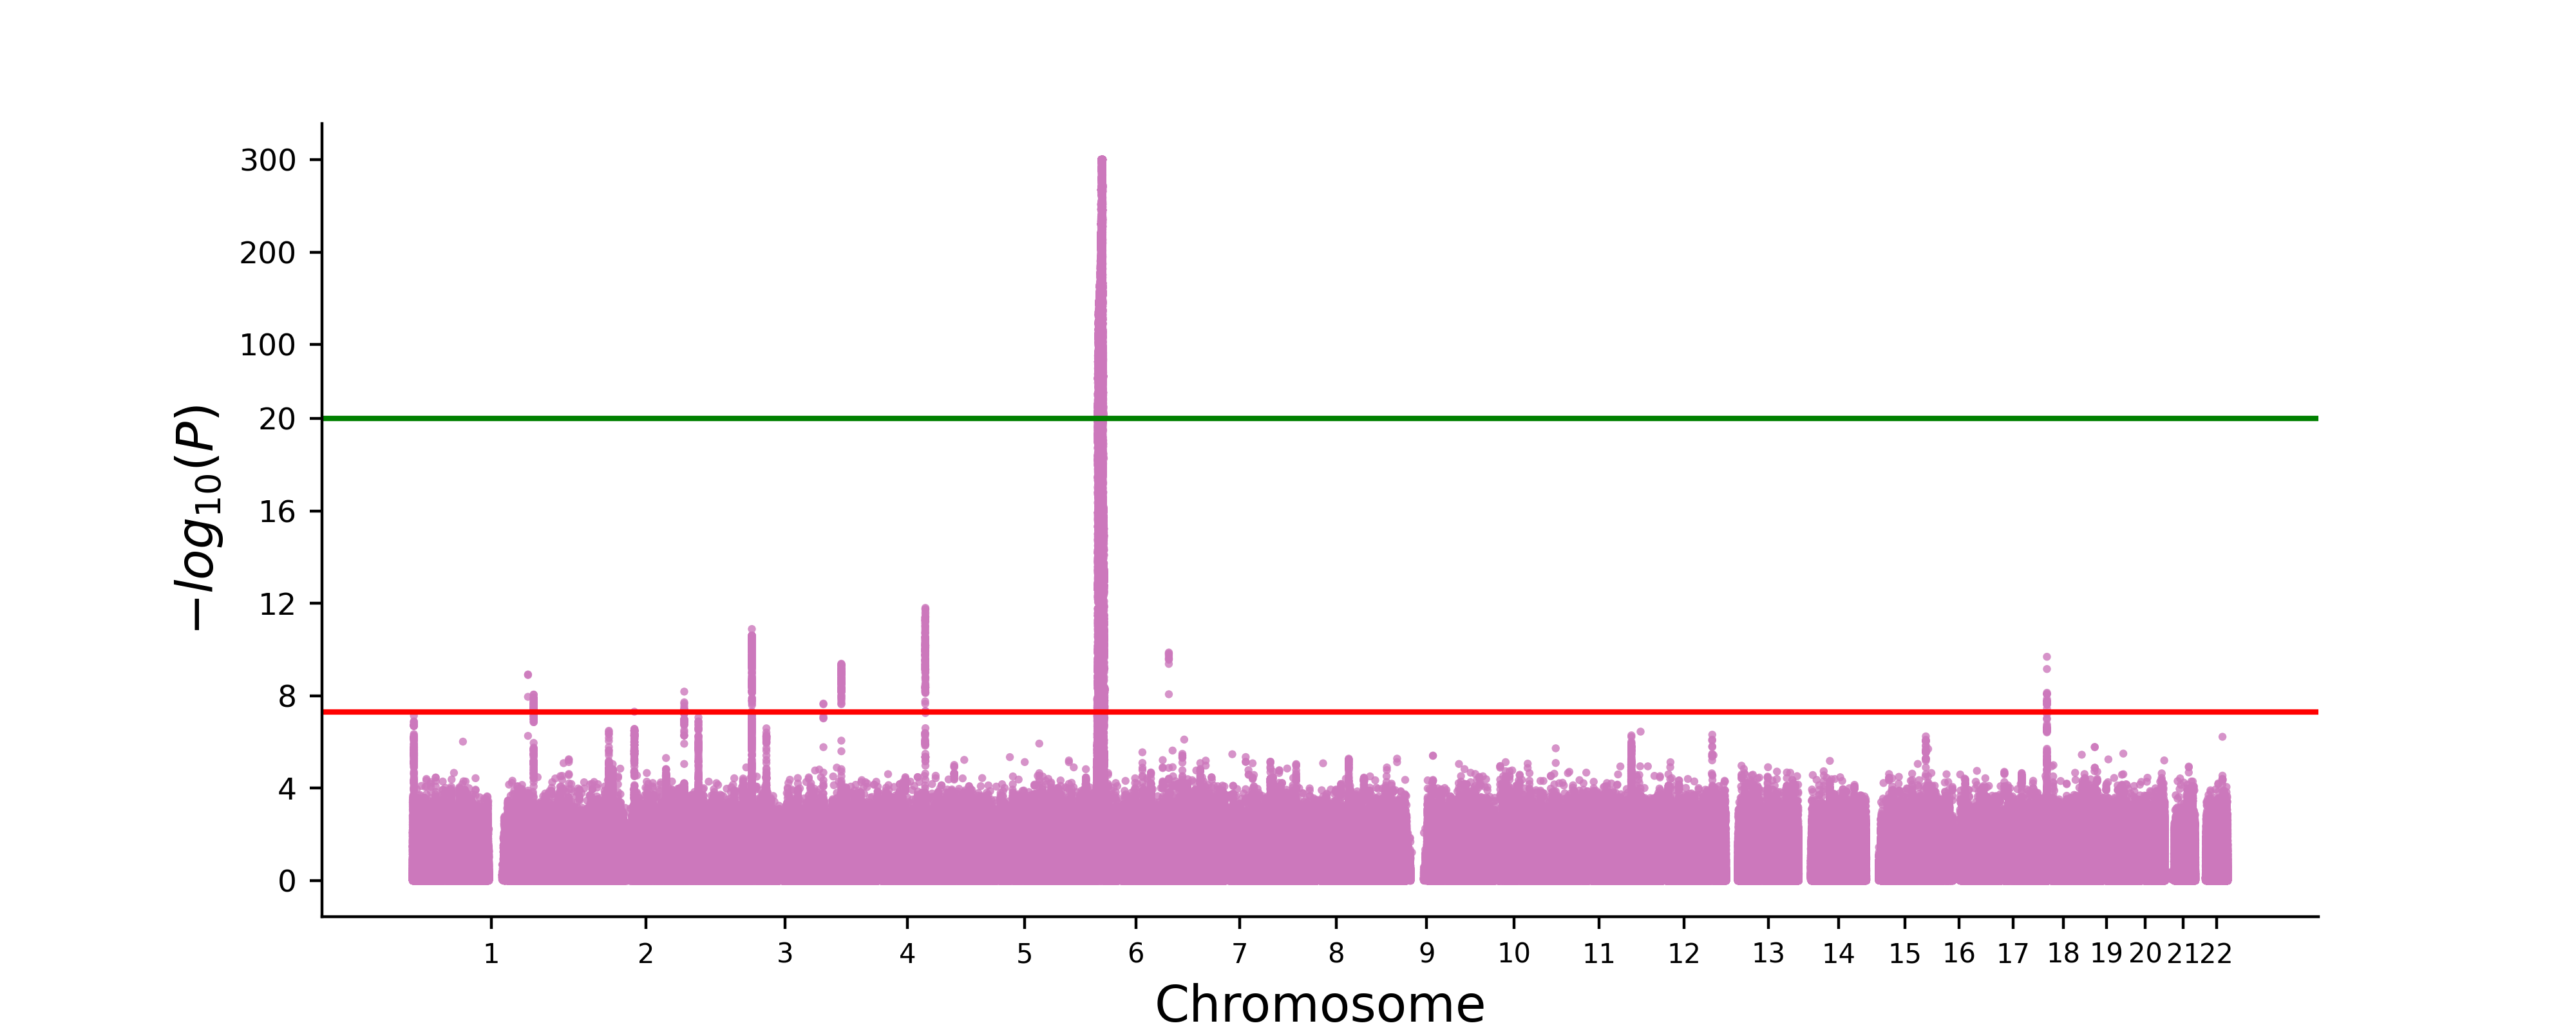
\includegraphics[width=\textwidth]{figures/manhattan_bin/fastgwa_400k17.png}
    \end{subfigure}%
    \begin{subfigure}{.5\textwidth}
    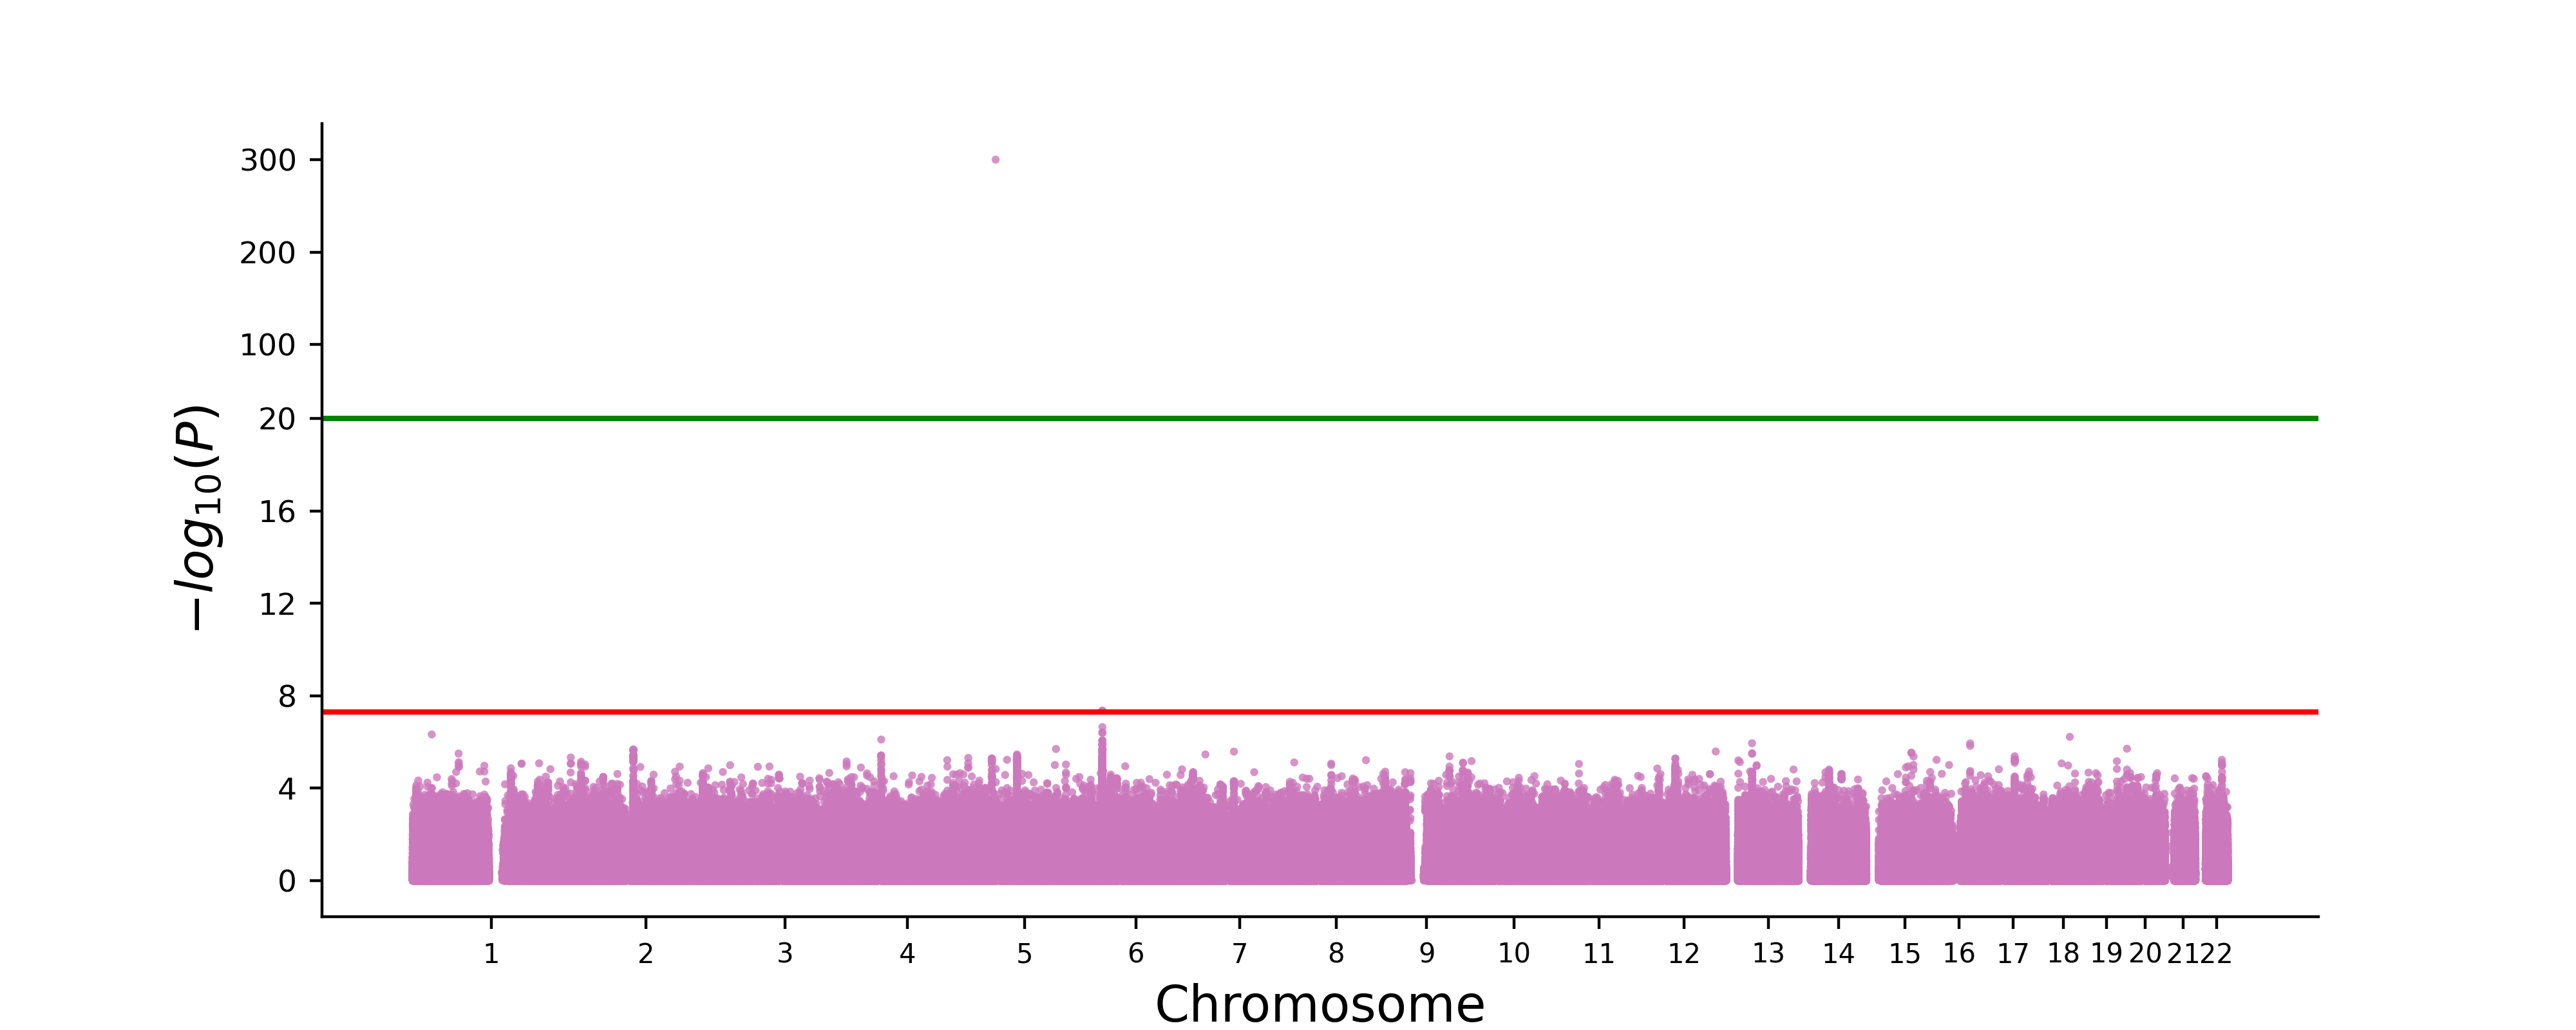
\includegraphics[width=\textwidth]{figures/manhattan_bin/fastgwa_400k22.png}
    \end{subfigure}
    \begin{subfigure}{.5\textwidth}
    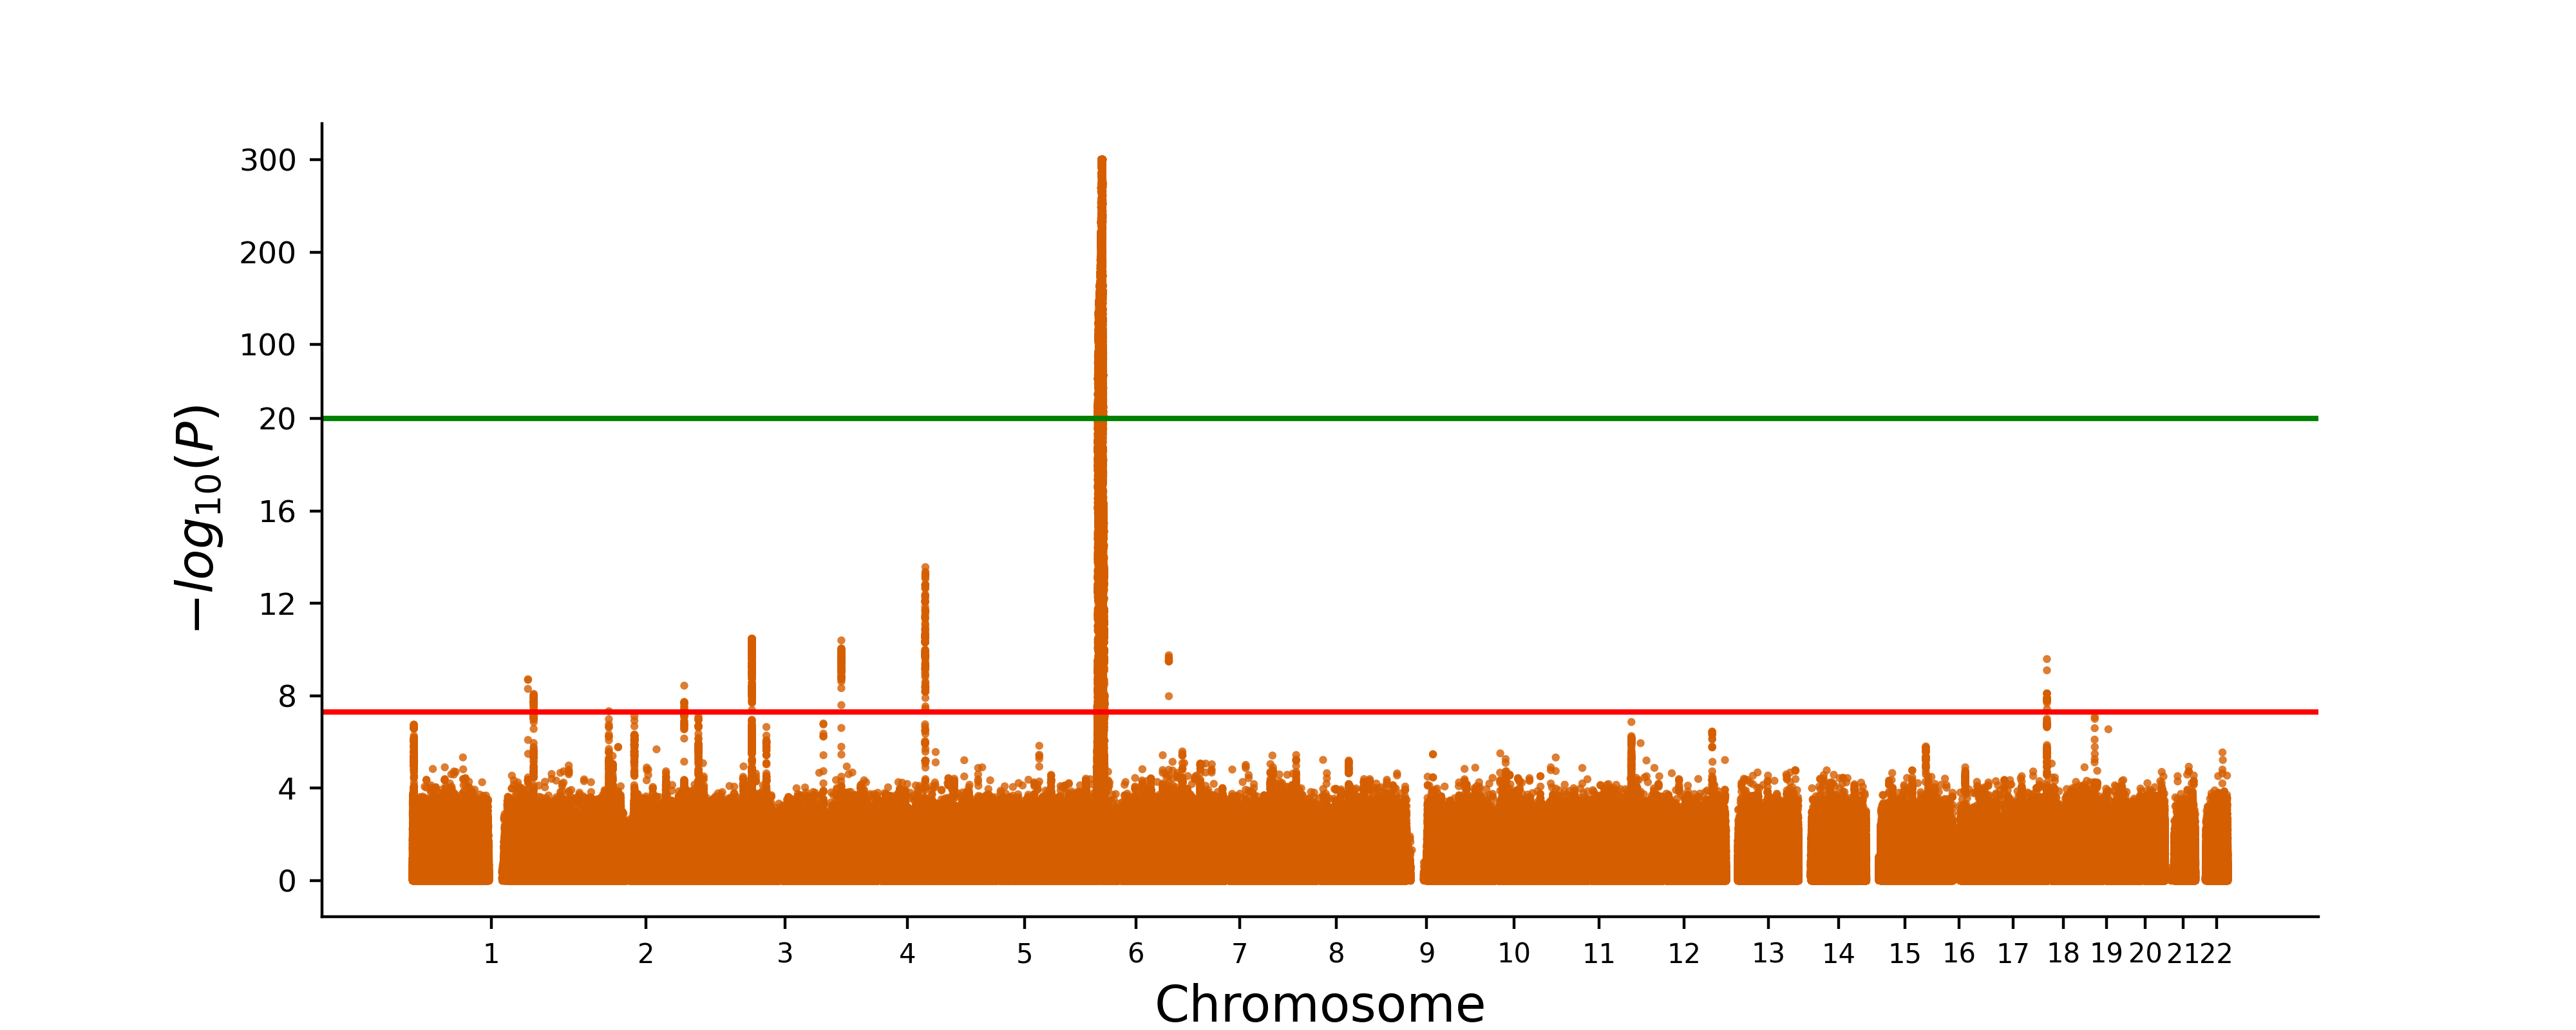
\includegraphics[width=\textwidth]{figures/manhattan_bin/regenie_400kCoeliac_disease.png}
    \end{subfigure}%
    \begin{subfigure}{.5\textwidth}
    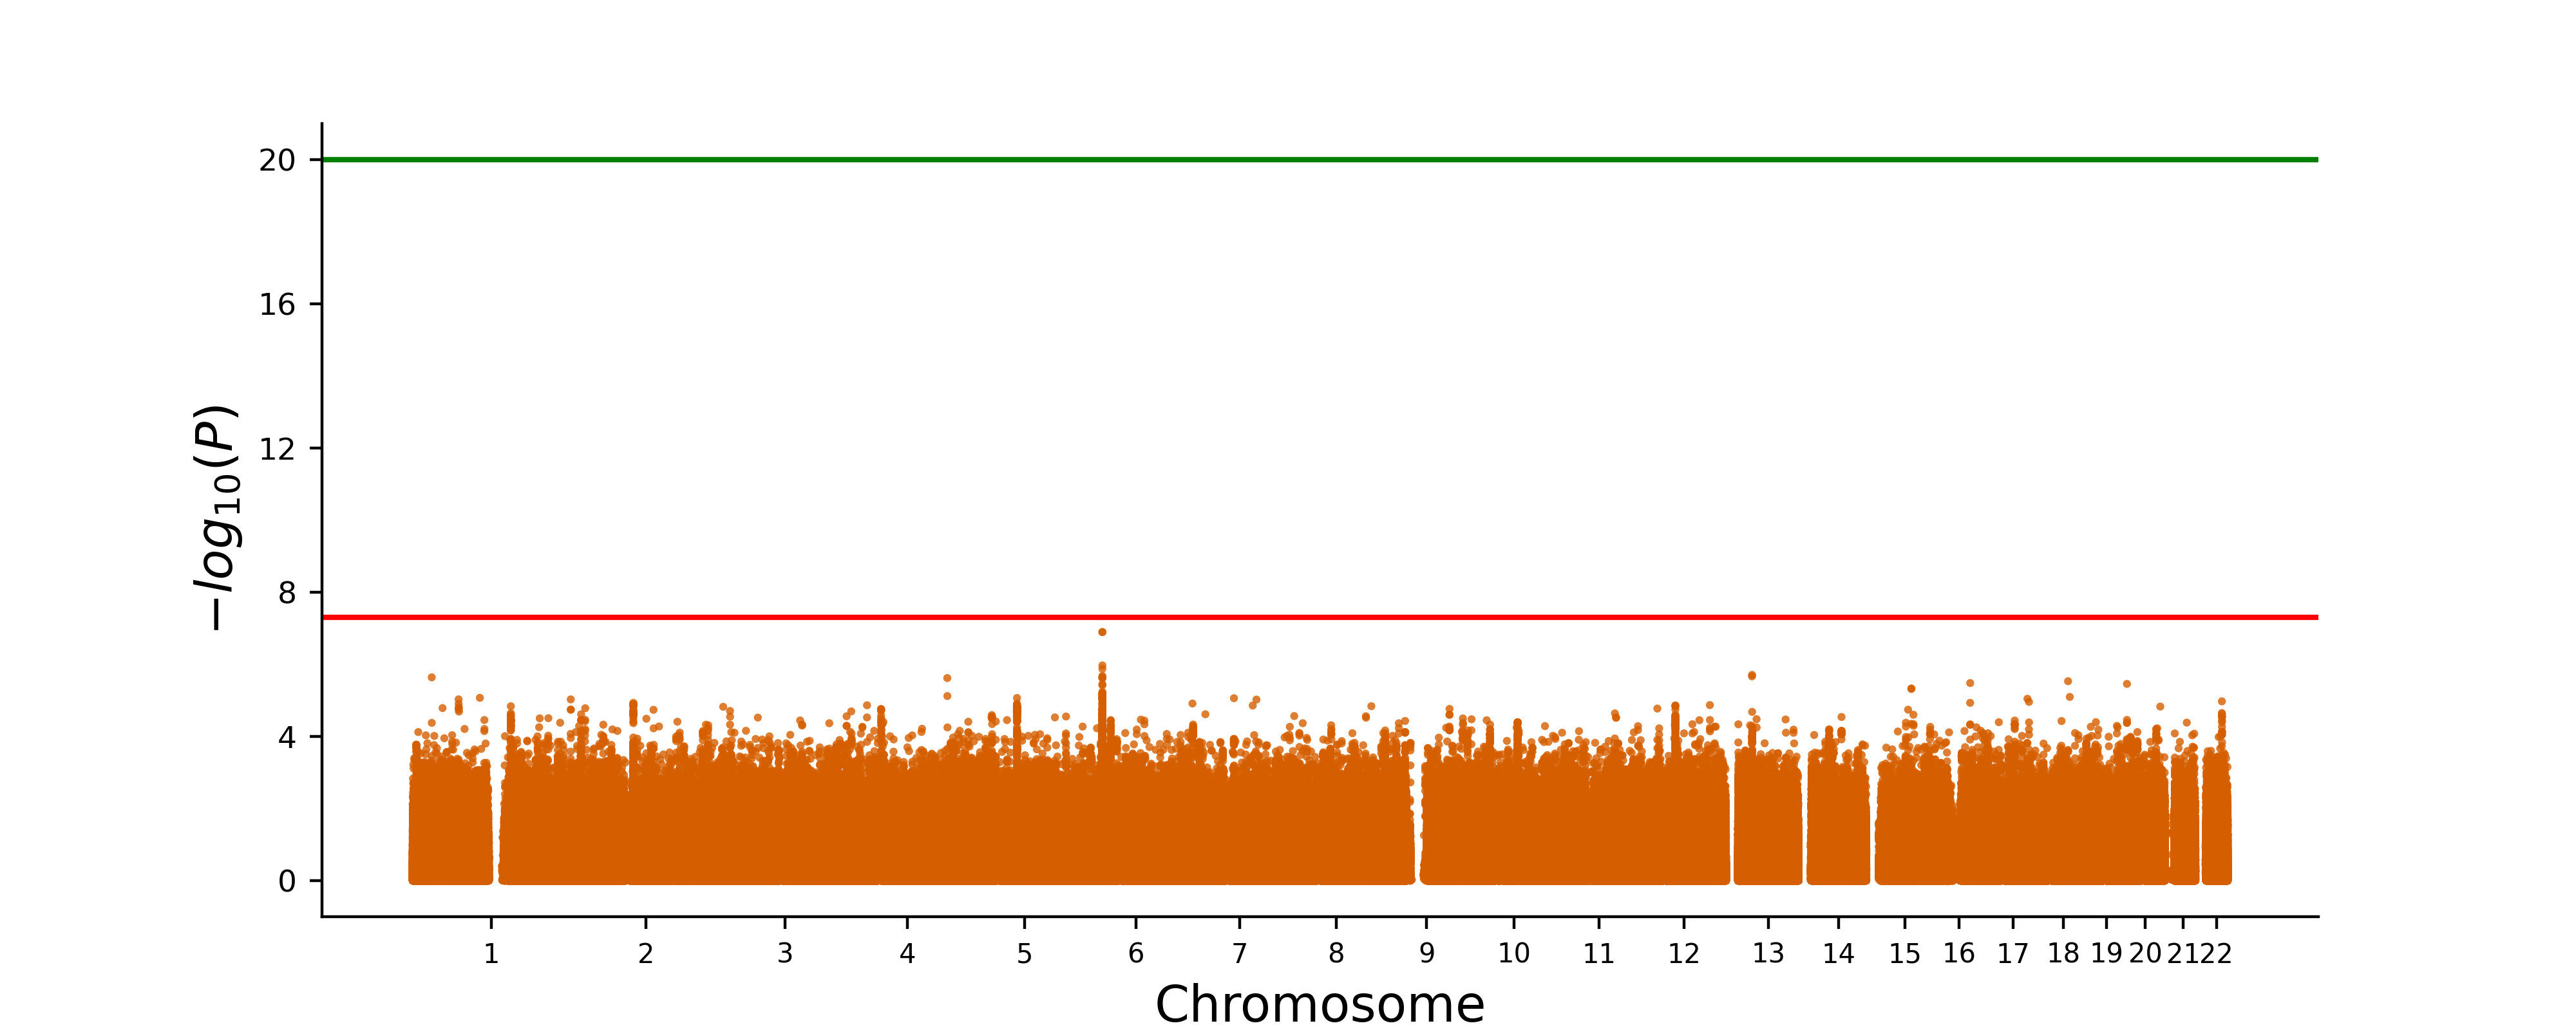
\includegraphics[width=\textwidth]{figures/manhattan_bin/regenie_400kVitiligo.png}
    \end{subfigure}
    \begin{subfigure}{.5\textwidth}
    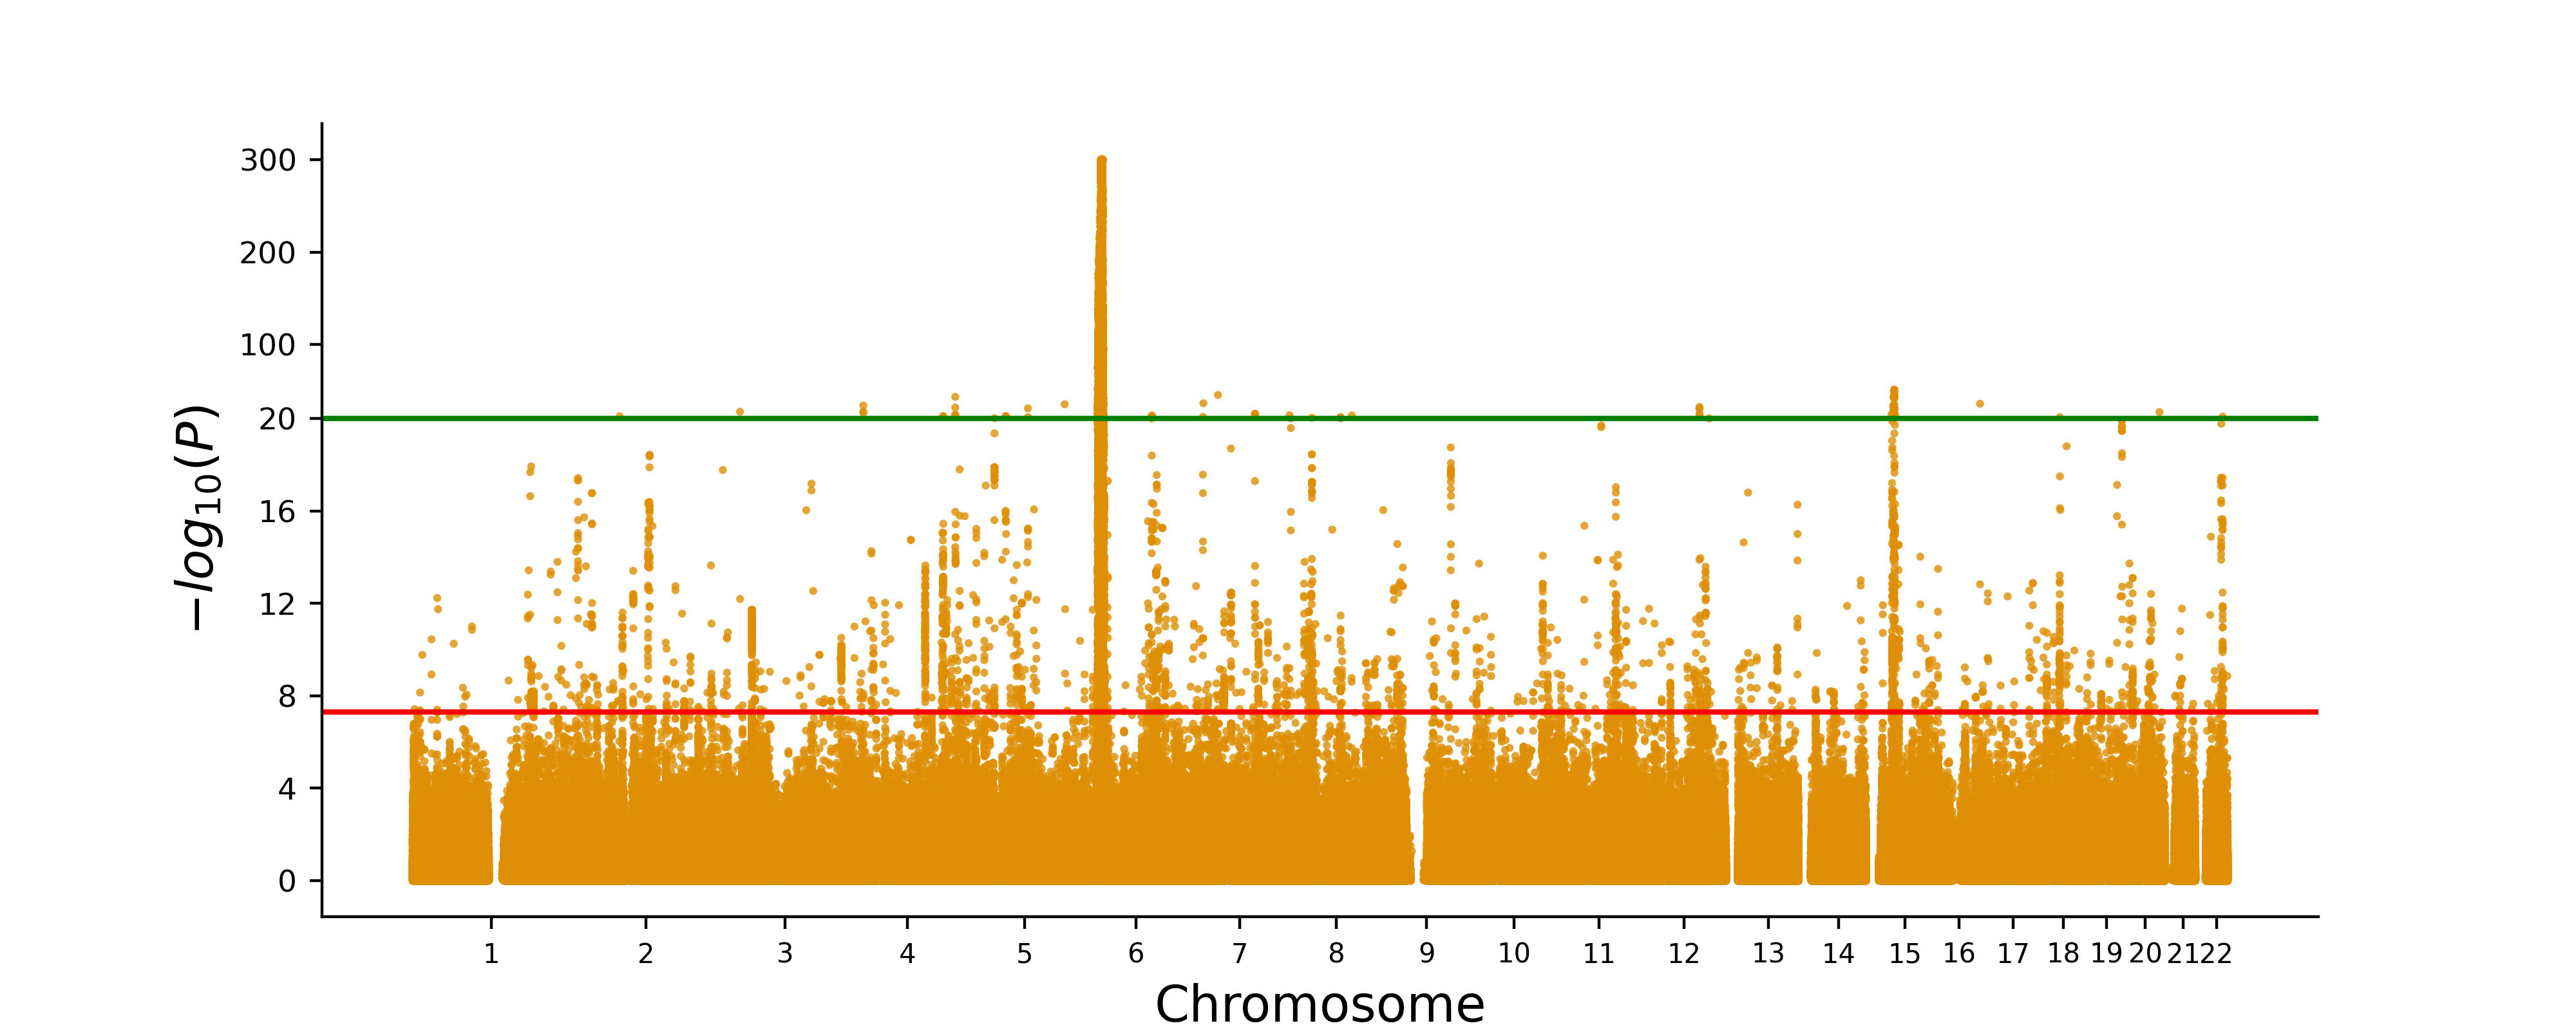
\includegraphics[width=\textwidth]{figures/manhattan_bin/imputed_bgen_bolt_2.sumstats.gz.png}
    \end{subfigure}%
    \begin{subfigure}{.5\textwidth}
    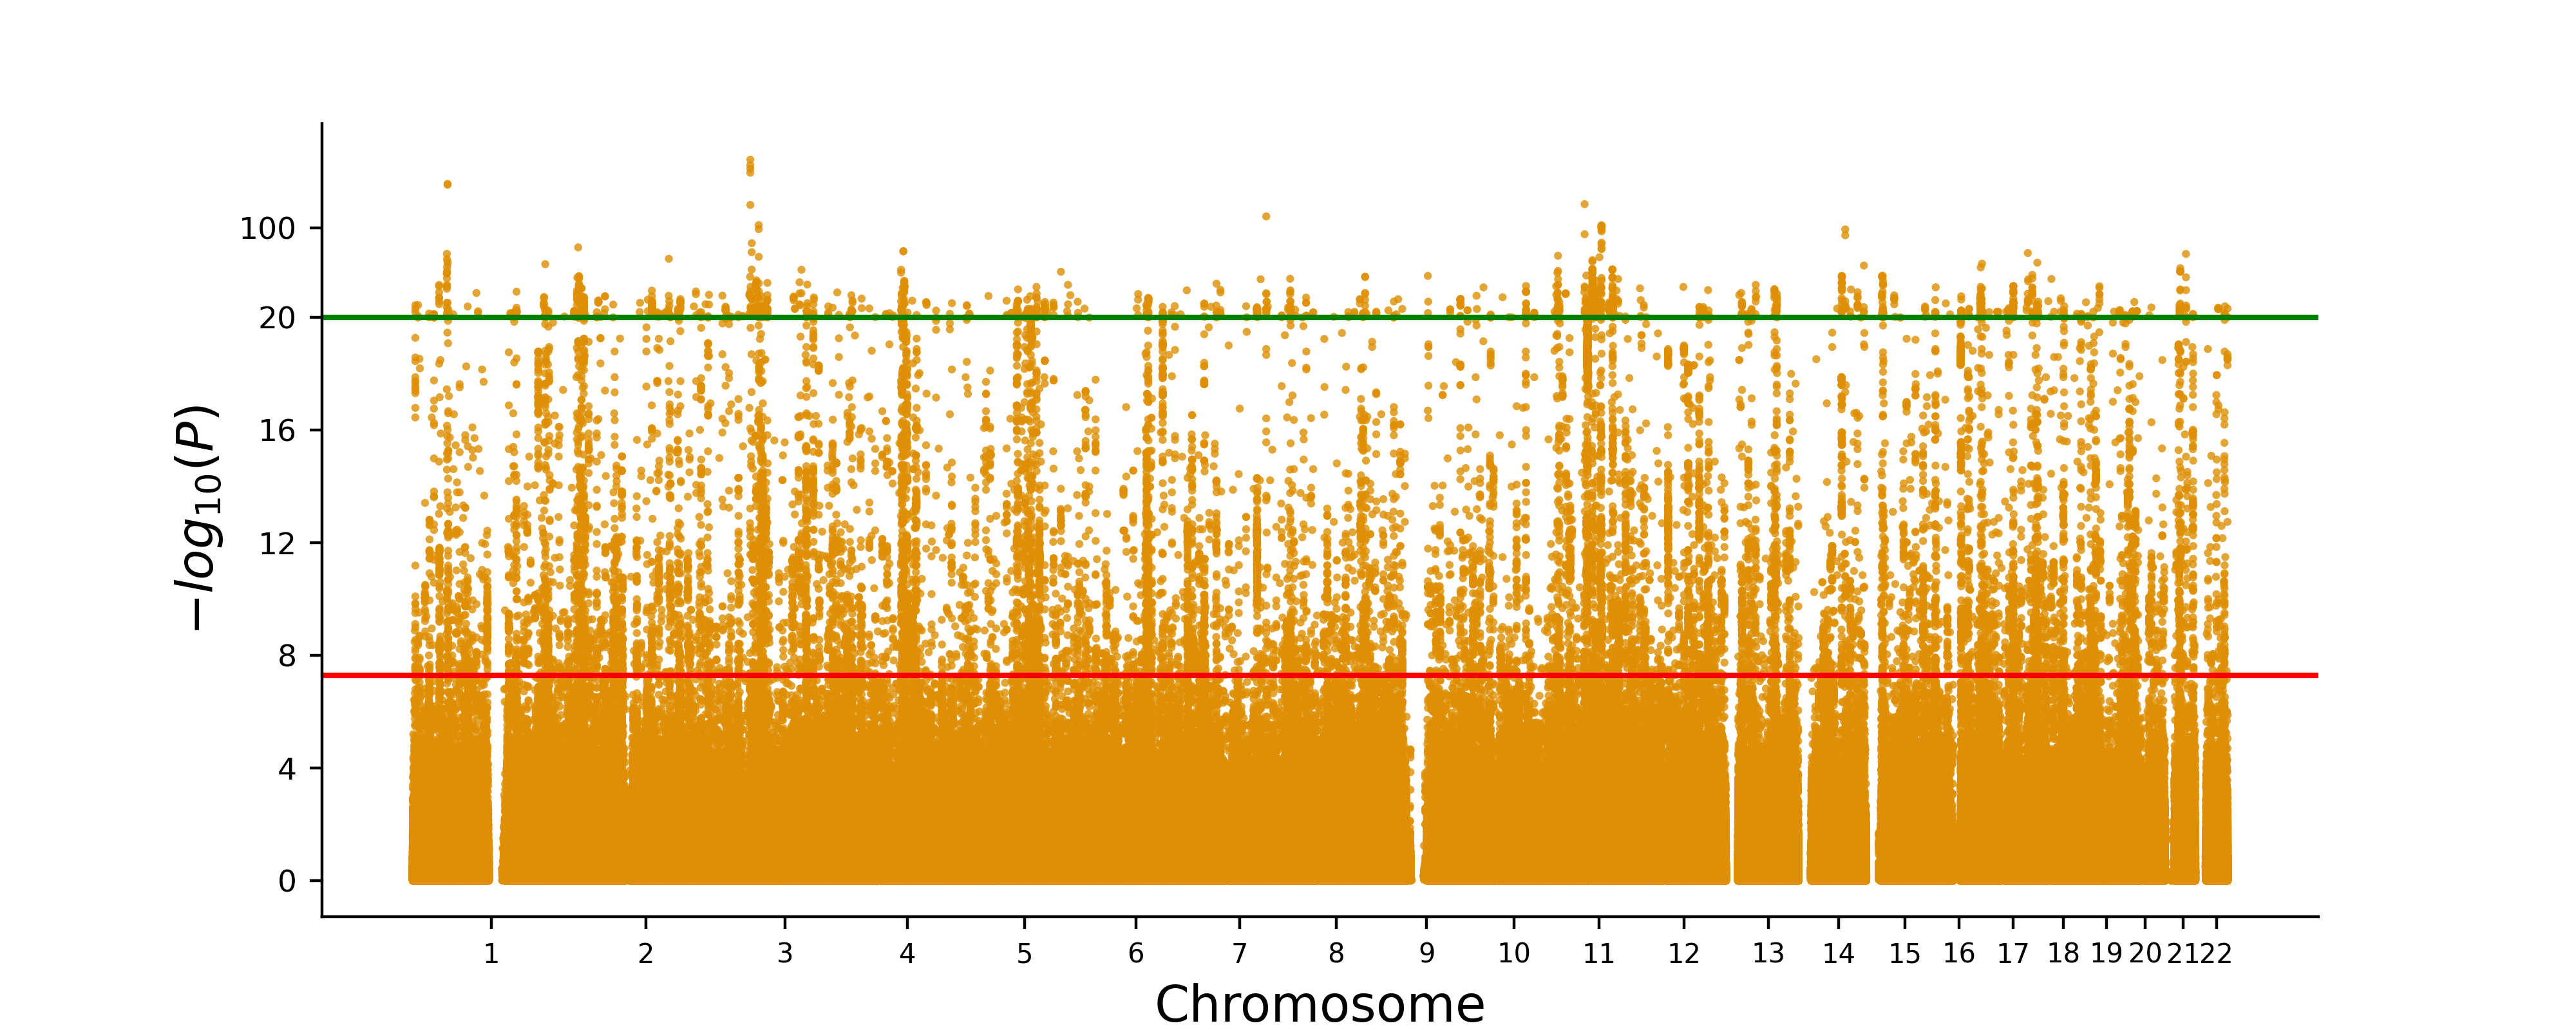
\includegraphics[width=\textwidth]{figures/manhattan_bin/imputed_bgen_bolt_3.sumstats.gz.png}
    \end{subfigure}
    \begin{subfigure}{.5\textwidth}
    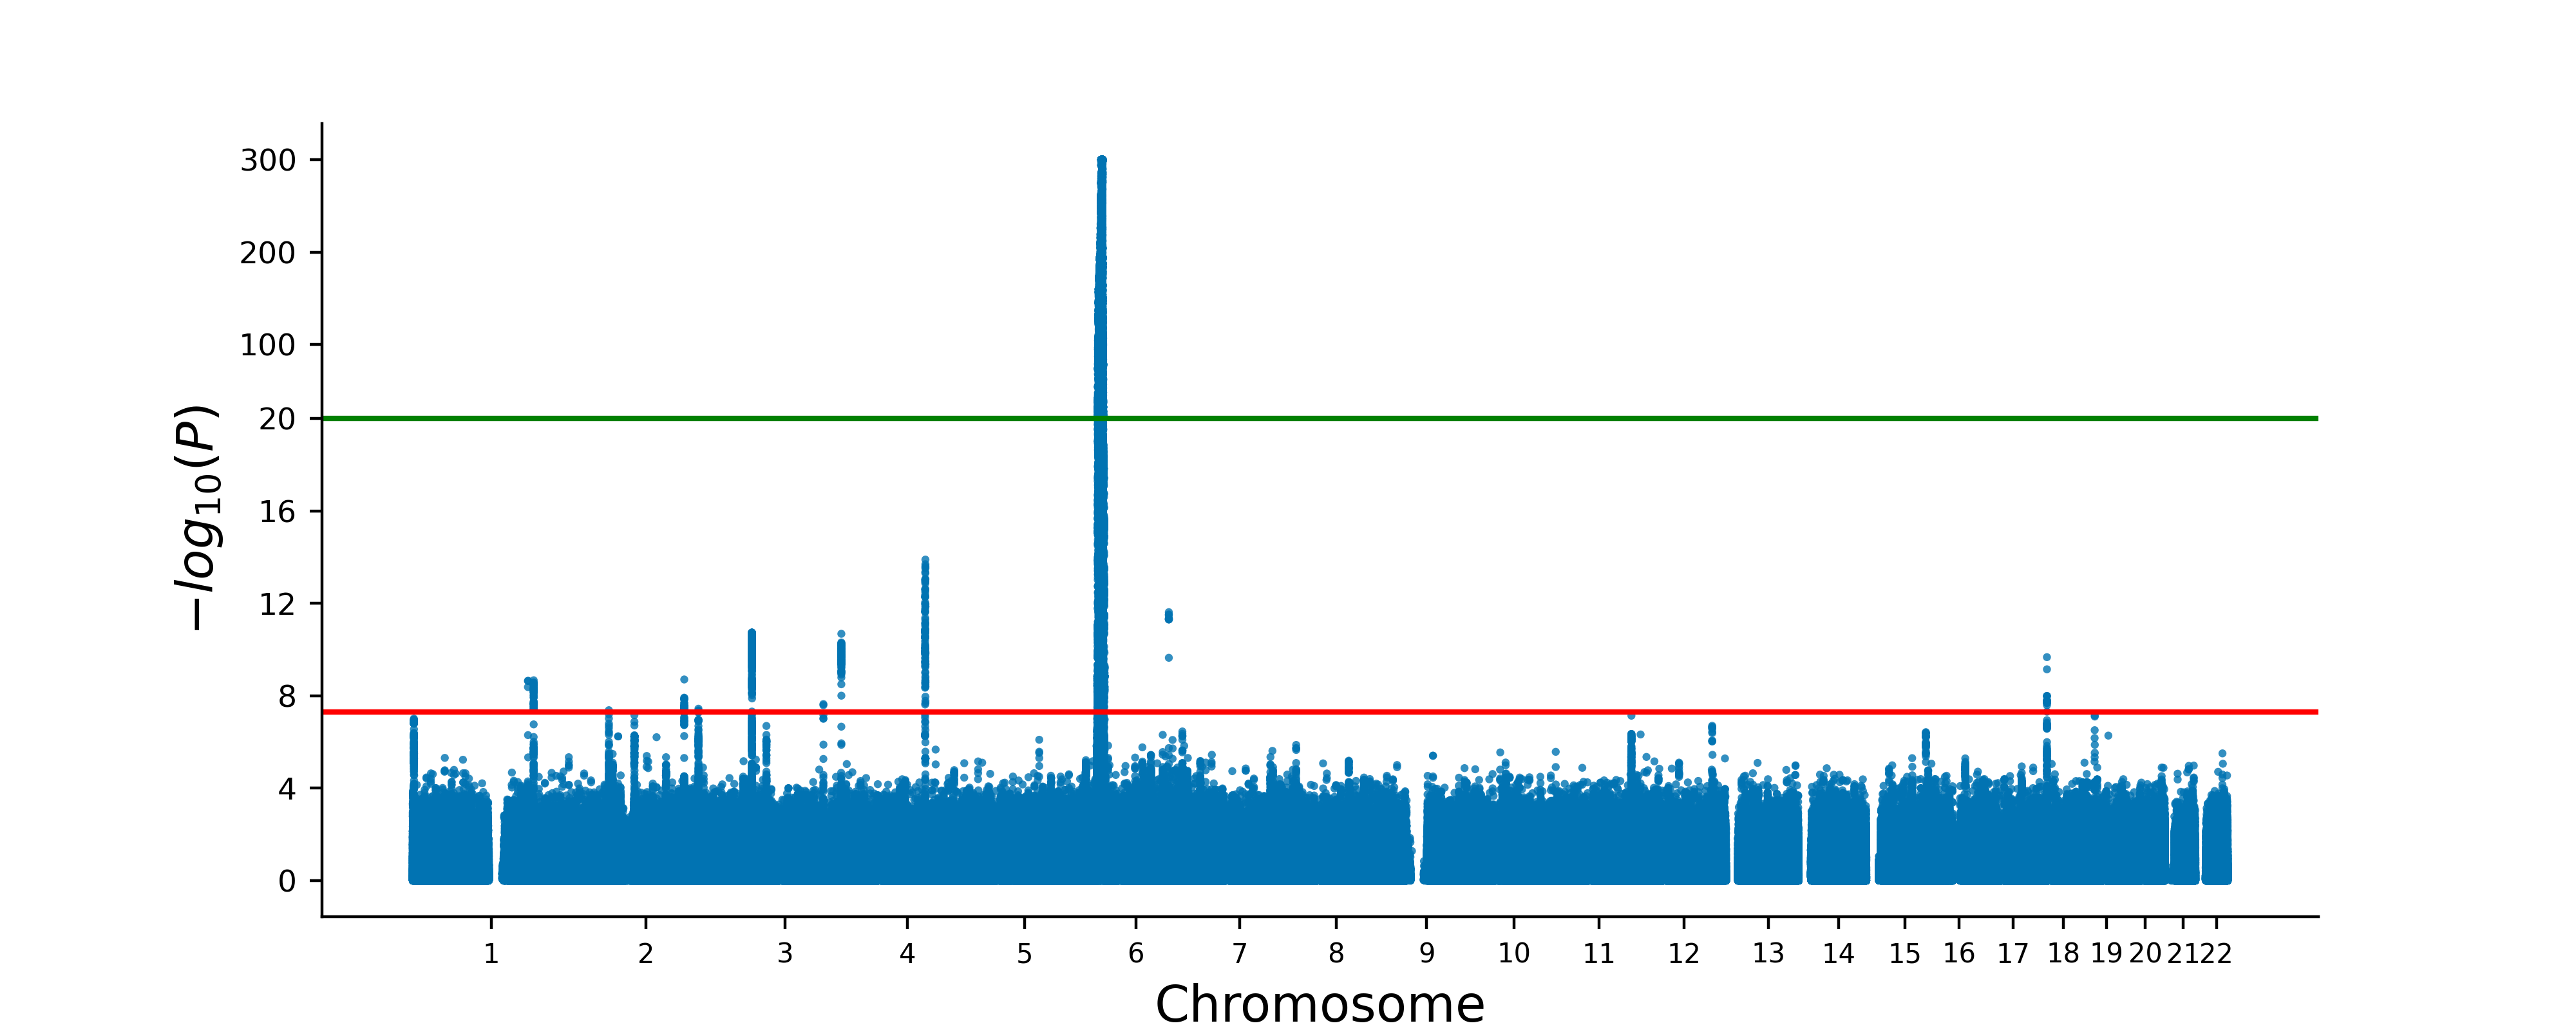
\includegraphics[width=\textwidth]{figures/manhattan_bin/qd_Coeliac_disease.sumstats.gz.png}
    \caption{}
    \end{subfigure}%
    \begin{subfigure}{.5\textwidth}
    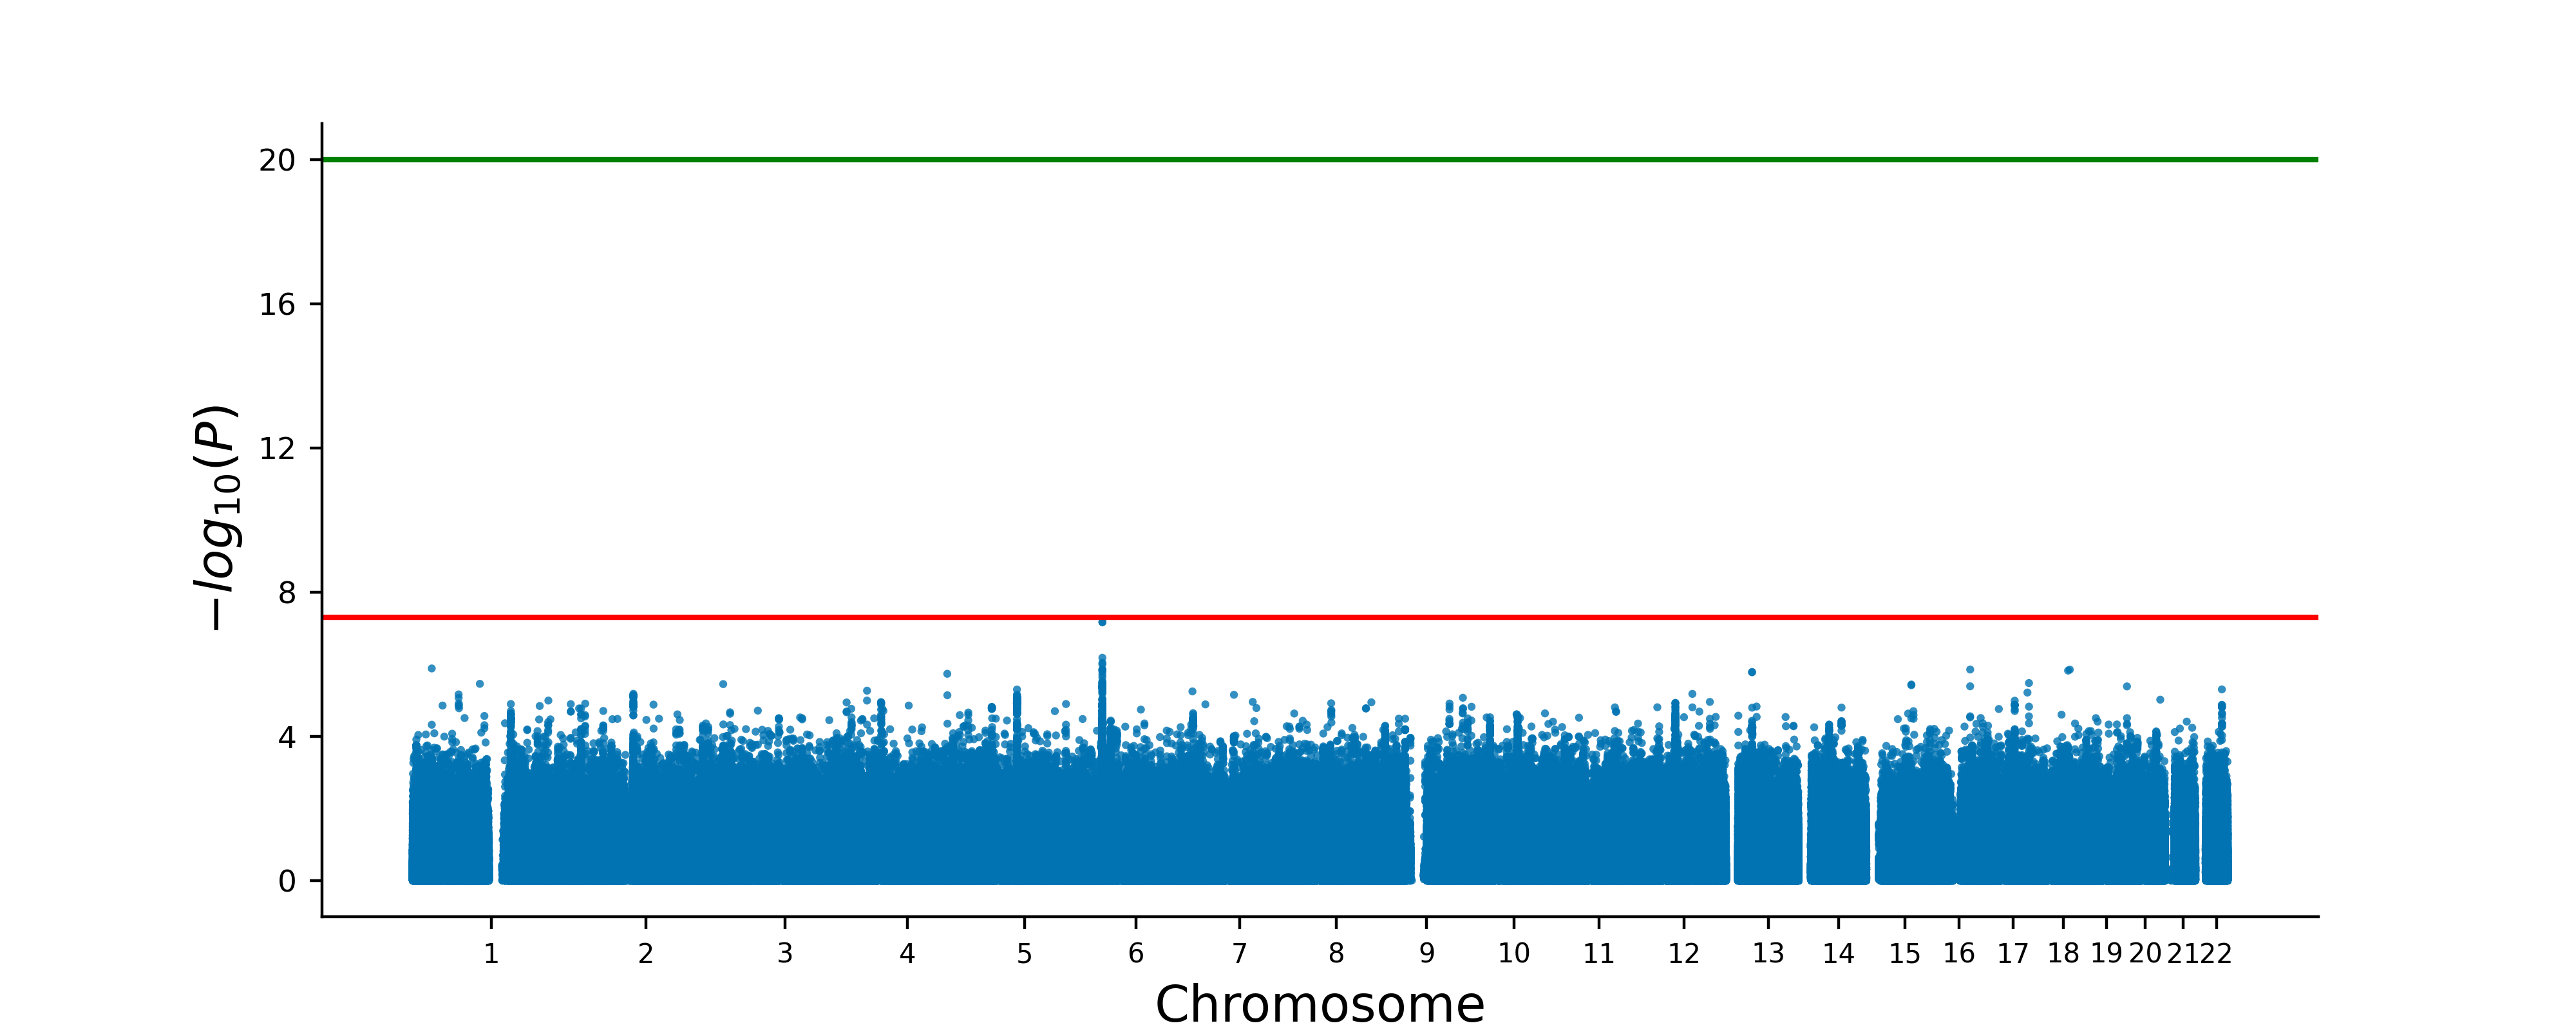
\includegraphics[width=\textwidth]{figures/manhattan_bin/qd_Vitiligo.sumstats.gz.png}
    \caption{}
    \end{subfigure}
    \caption{\textbf{Manhattan plots for two binary traits.}
    %
    (a) Celiac disease (prevalence $= 0.0047$) and (b) Vitiligo (prevalence $= 0.0005$).
    %
    ${\sim}13.3$ million variants were tested.
    %
    Red lines indicate a genome-wide significance threshold of $ P = 5 \times 10^{-8}$ and the green line indicates $P = 1 \times 10^{-20}$.    }
    \label{fig:qd_man_bin2}
\end{figure}


\begin{figure}[h!]
    \centering
    
\includegraphics[scale=0.425]{figures/manhattan_quant/legend.png}
    \begin{subfigure}{.5\textwidth}
    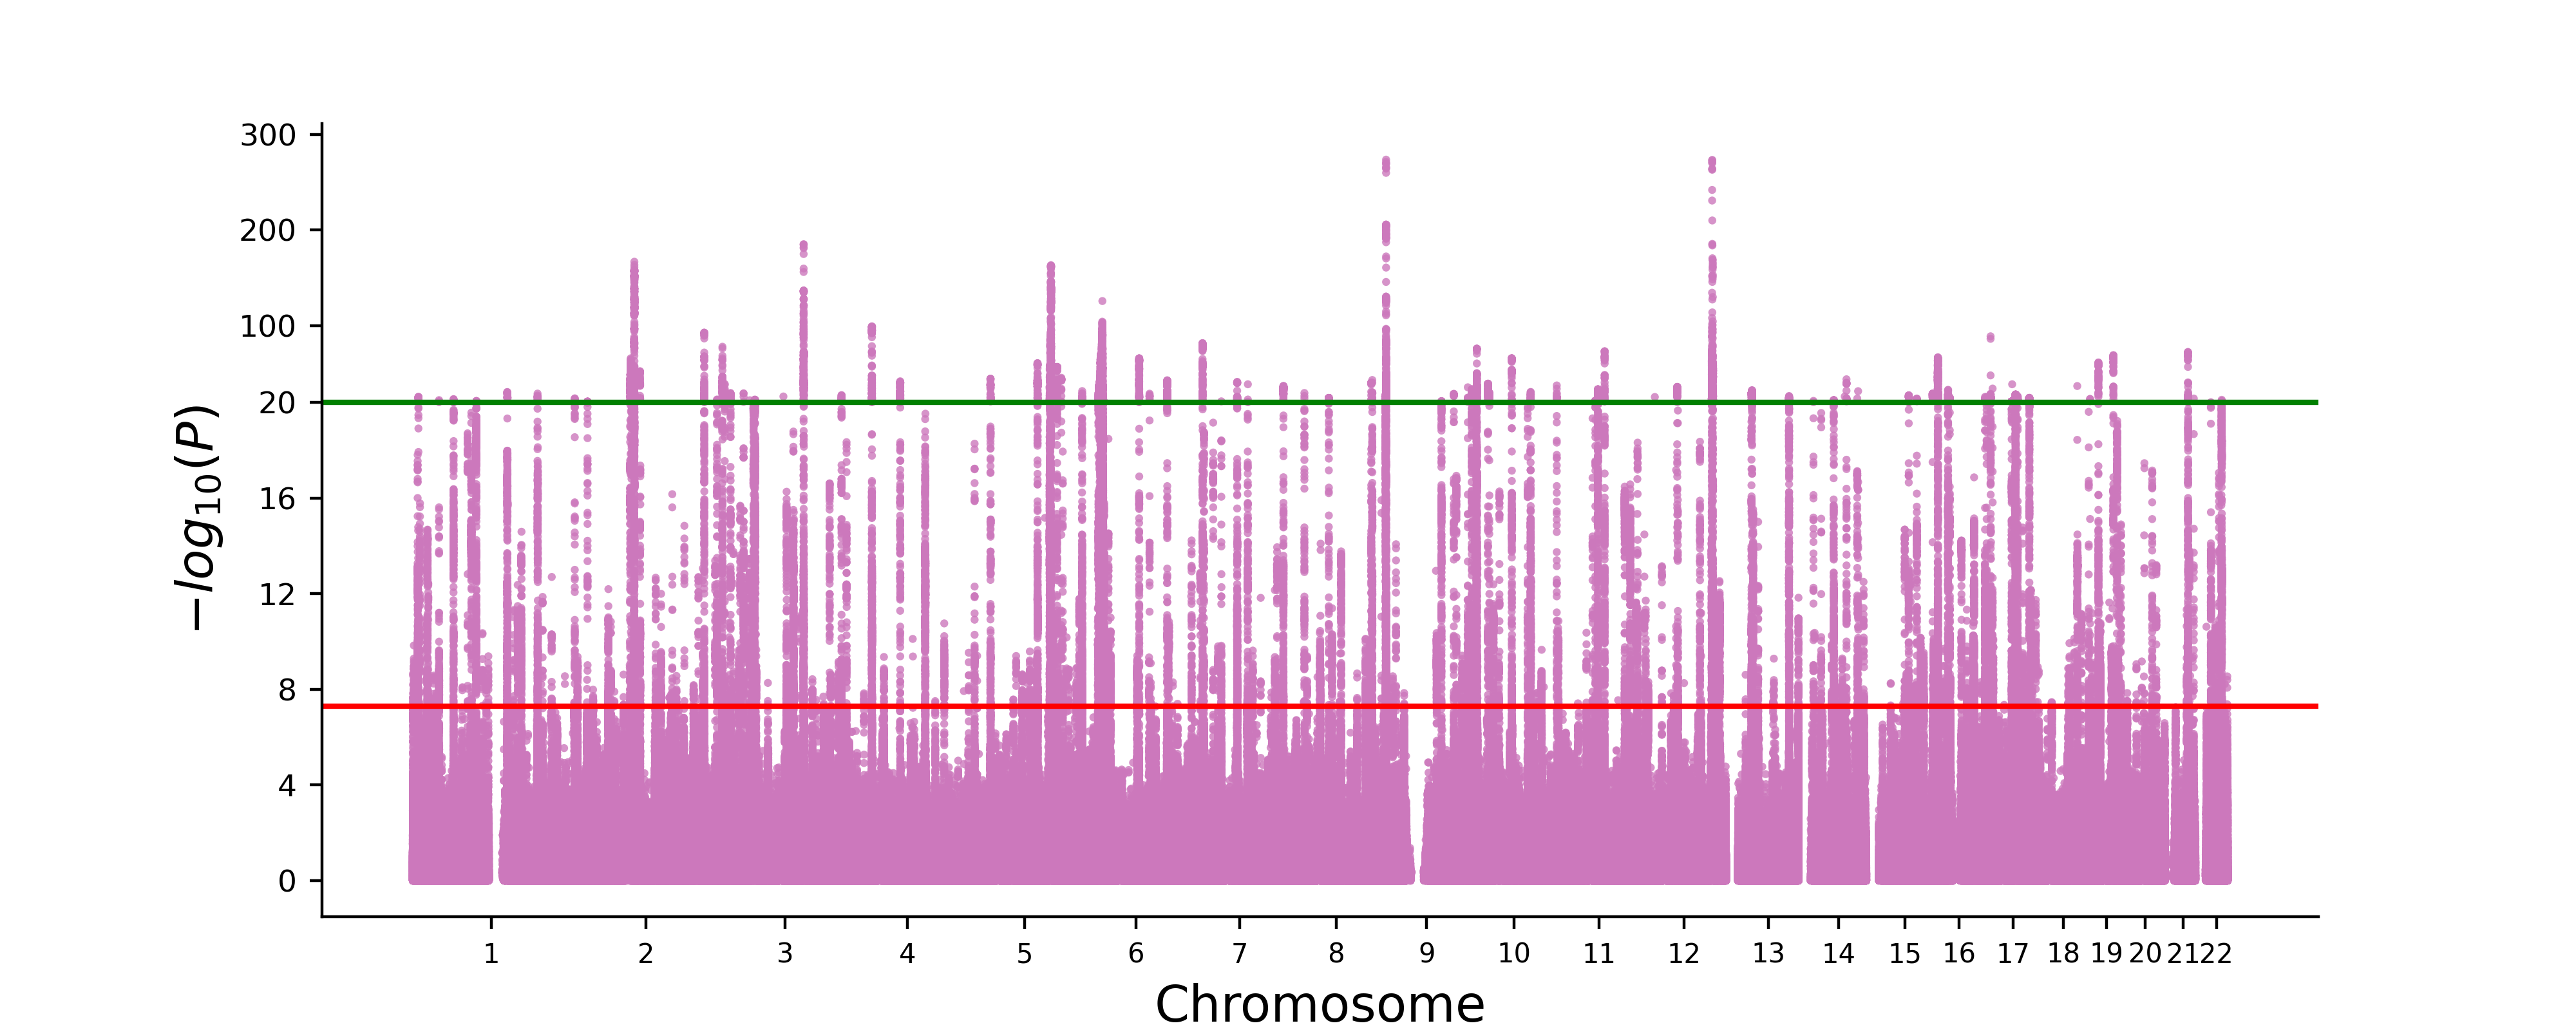
\includegraphics[width=\textwidth]{figures/manhattan_quant/imputed_fastgwa0.png}
    \end{subfigure}%
    \begin{subfigure}{.5\textwidth}
    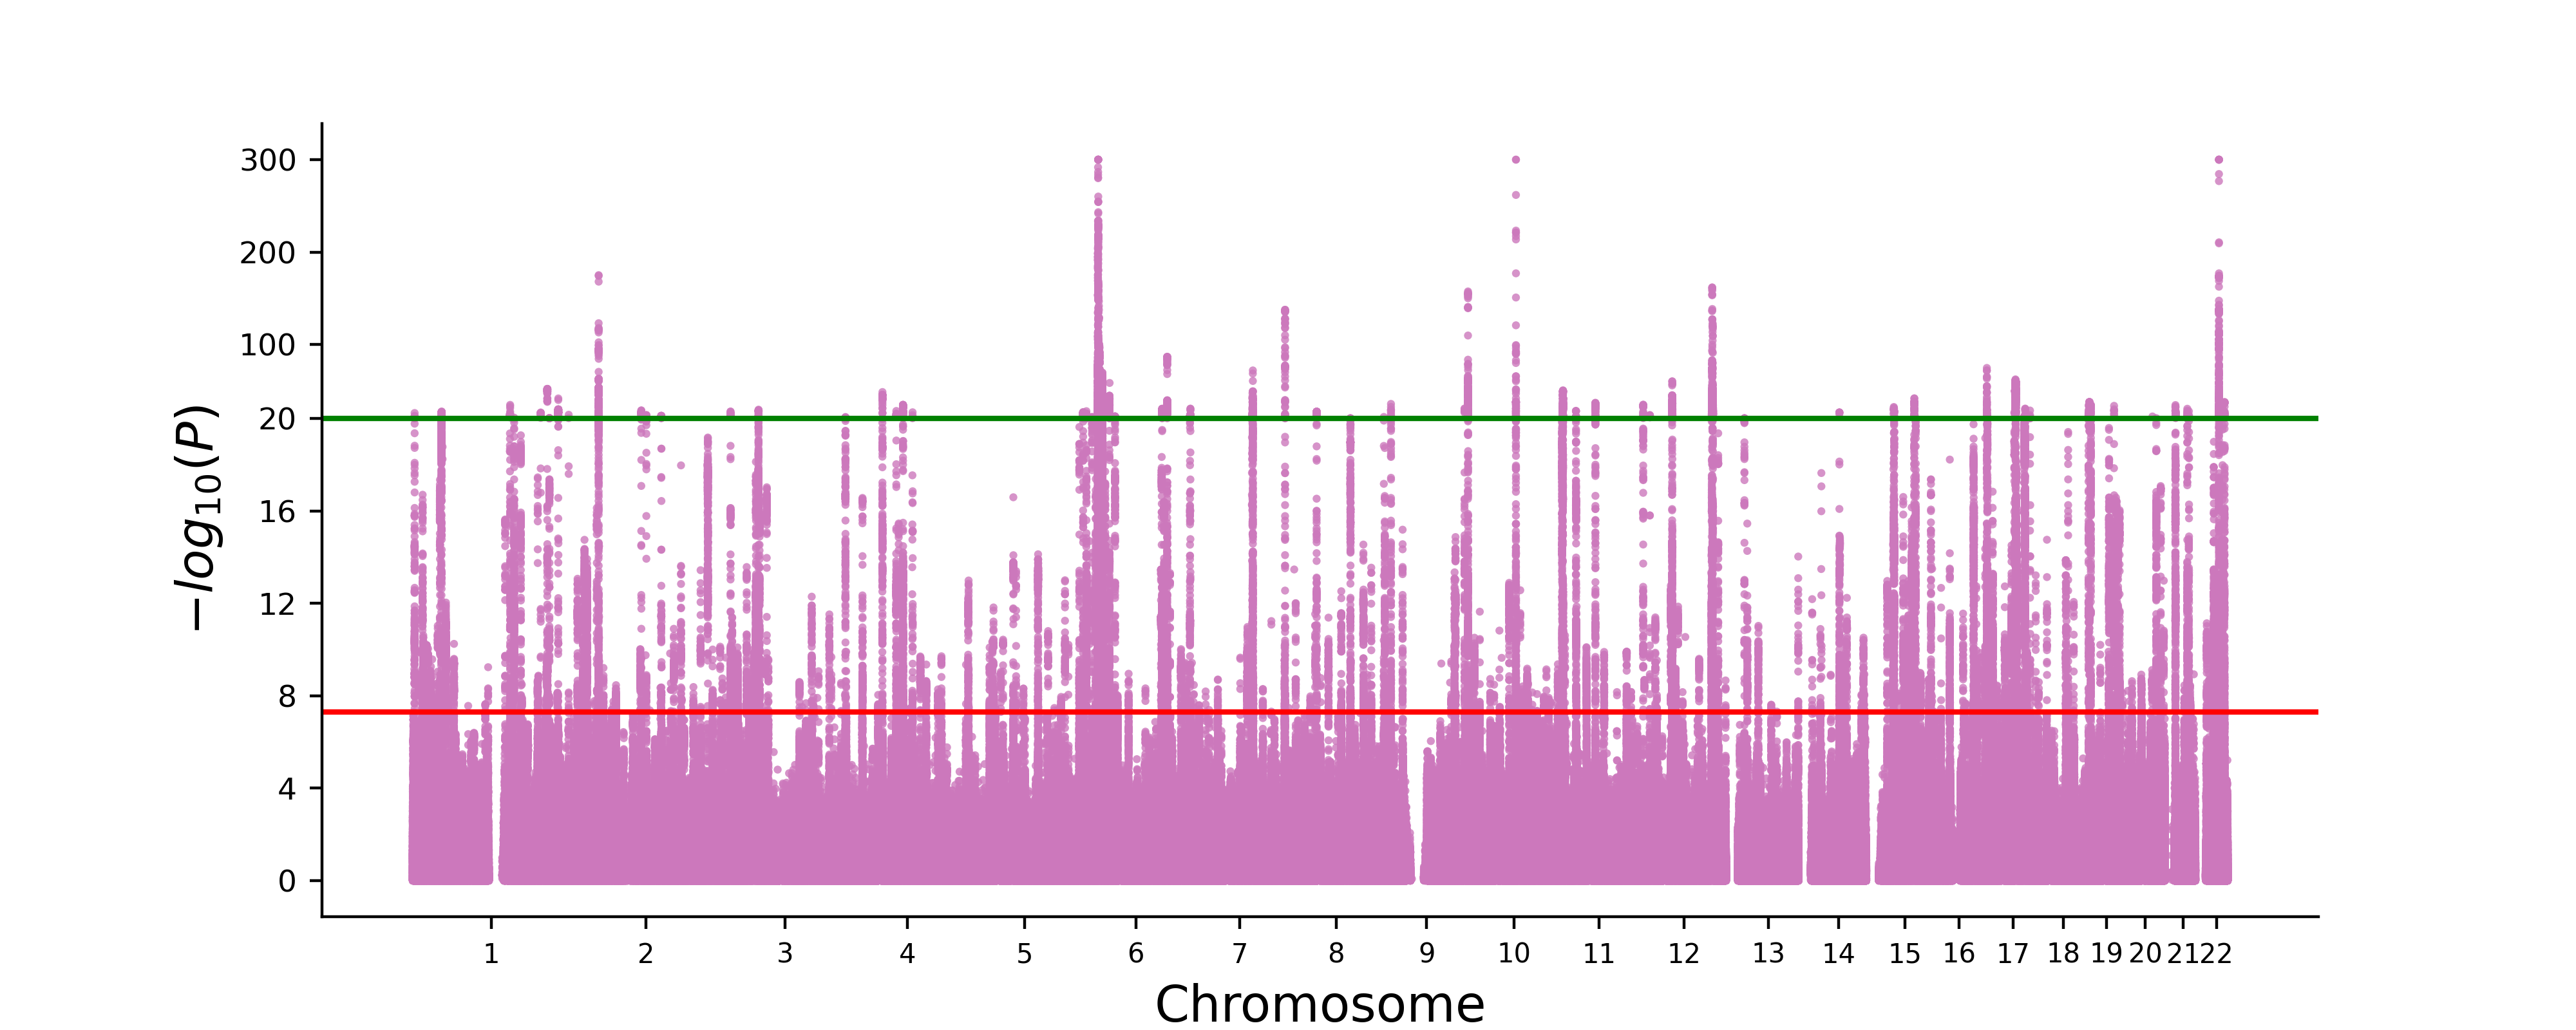
\includegraphics[width=\textwidth]{figures/manhattan_quant/imputed_fastgwa3.png}
    \end{subfigure}
    \begin{subfigure}{.5\textwidth}
    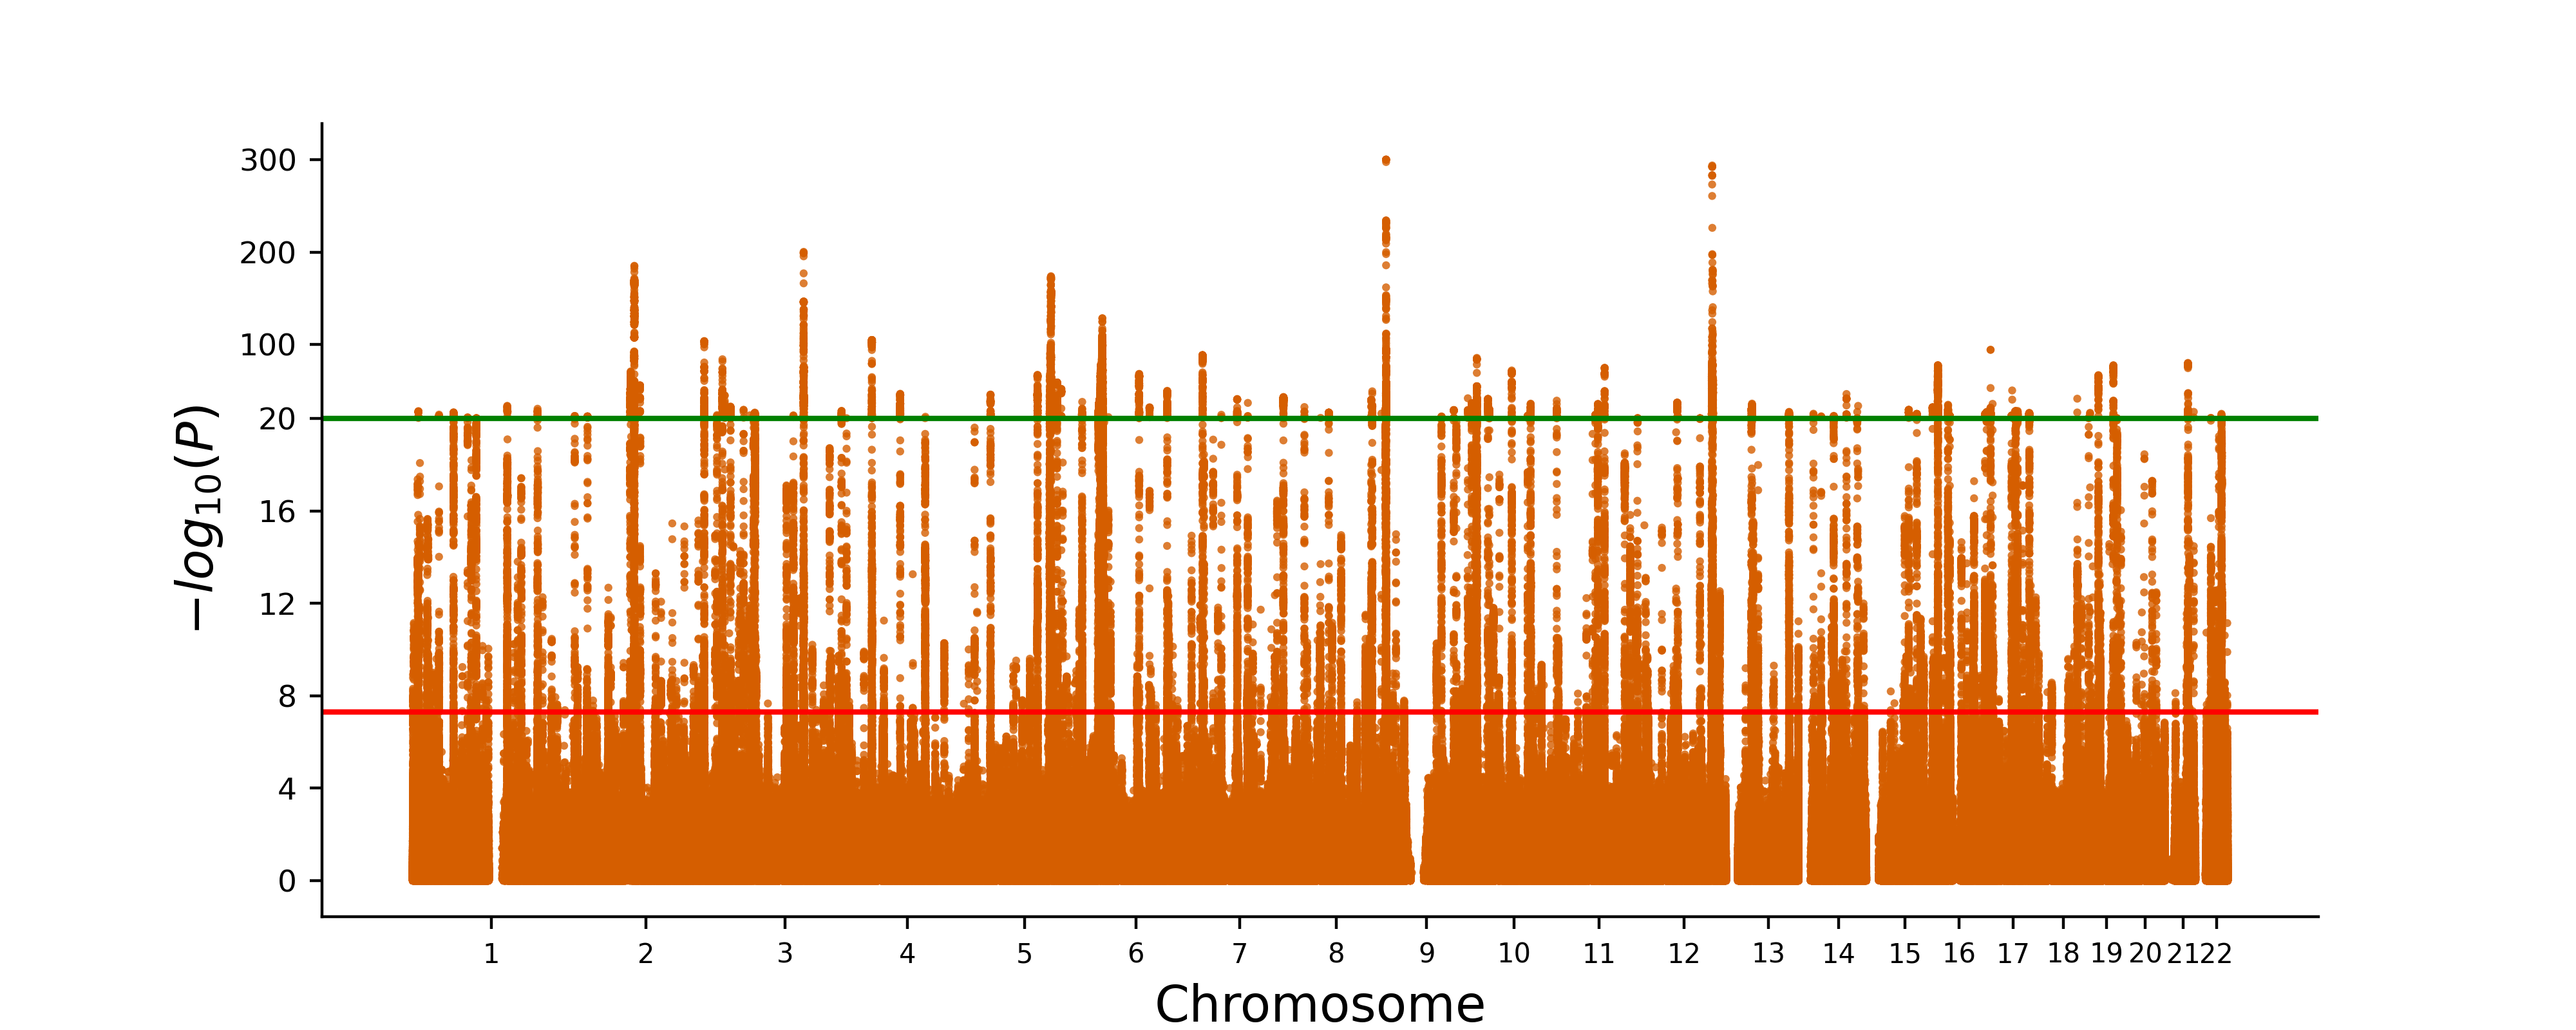
\includegraphics[width=\textwidth]{figures/manhattan_quant/regenie_400k_Eosinophill_count.regenie.png}
    \end{subfigure}%
    \begin{subfigure}{.5\textwidth}
    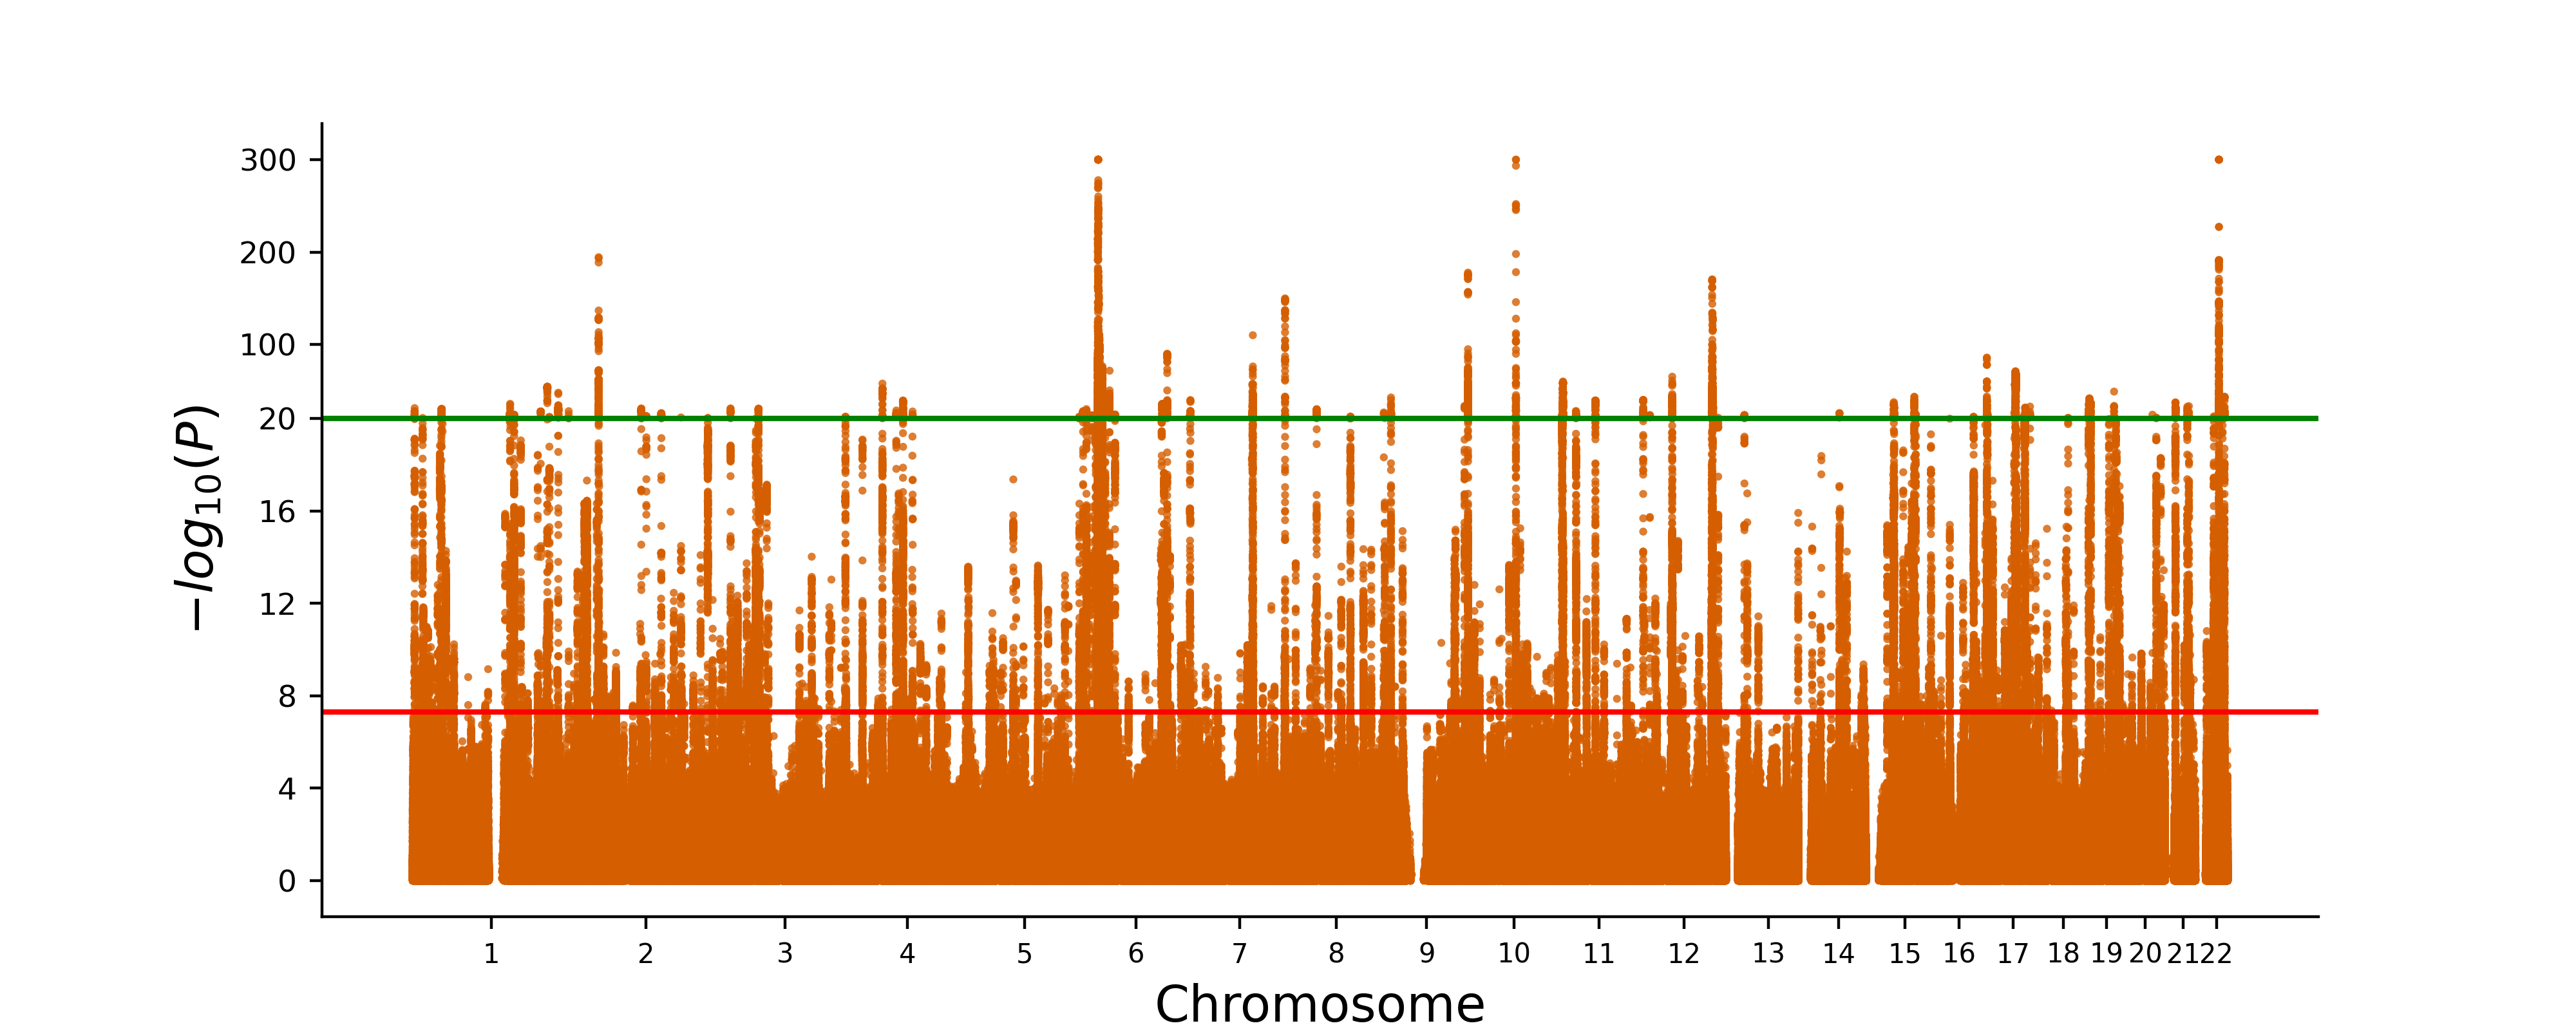
\includegraphics[width=\textwidth]{figures/manhattan_quant/regenie_400k_Haemoglobin_concentration.regenie.png}
    \end{subfigure}
    \begin{subfigure}{.5\textwidth}
    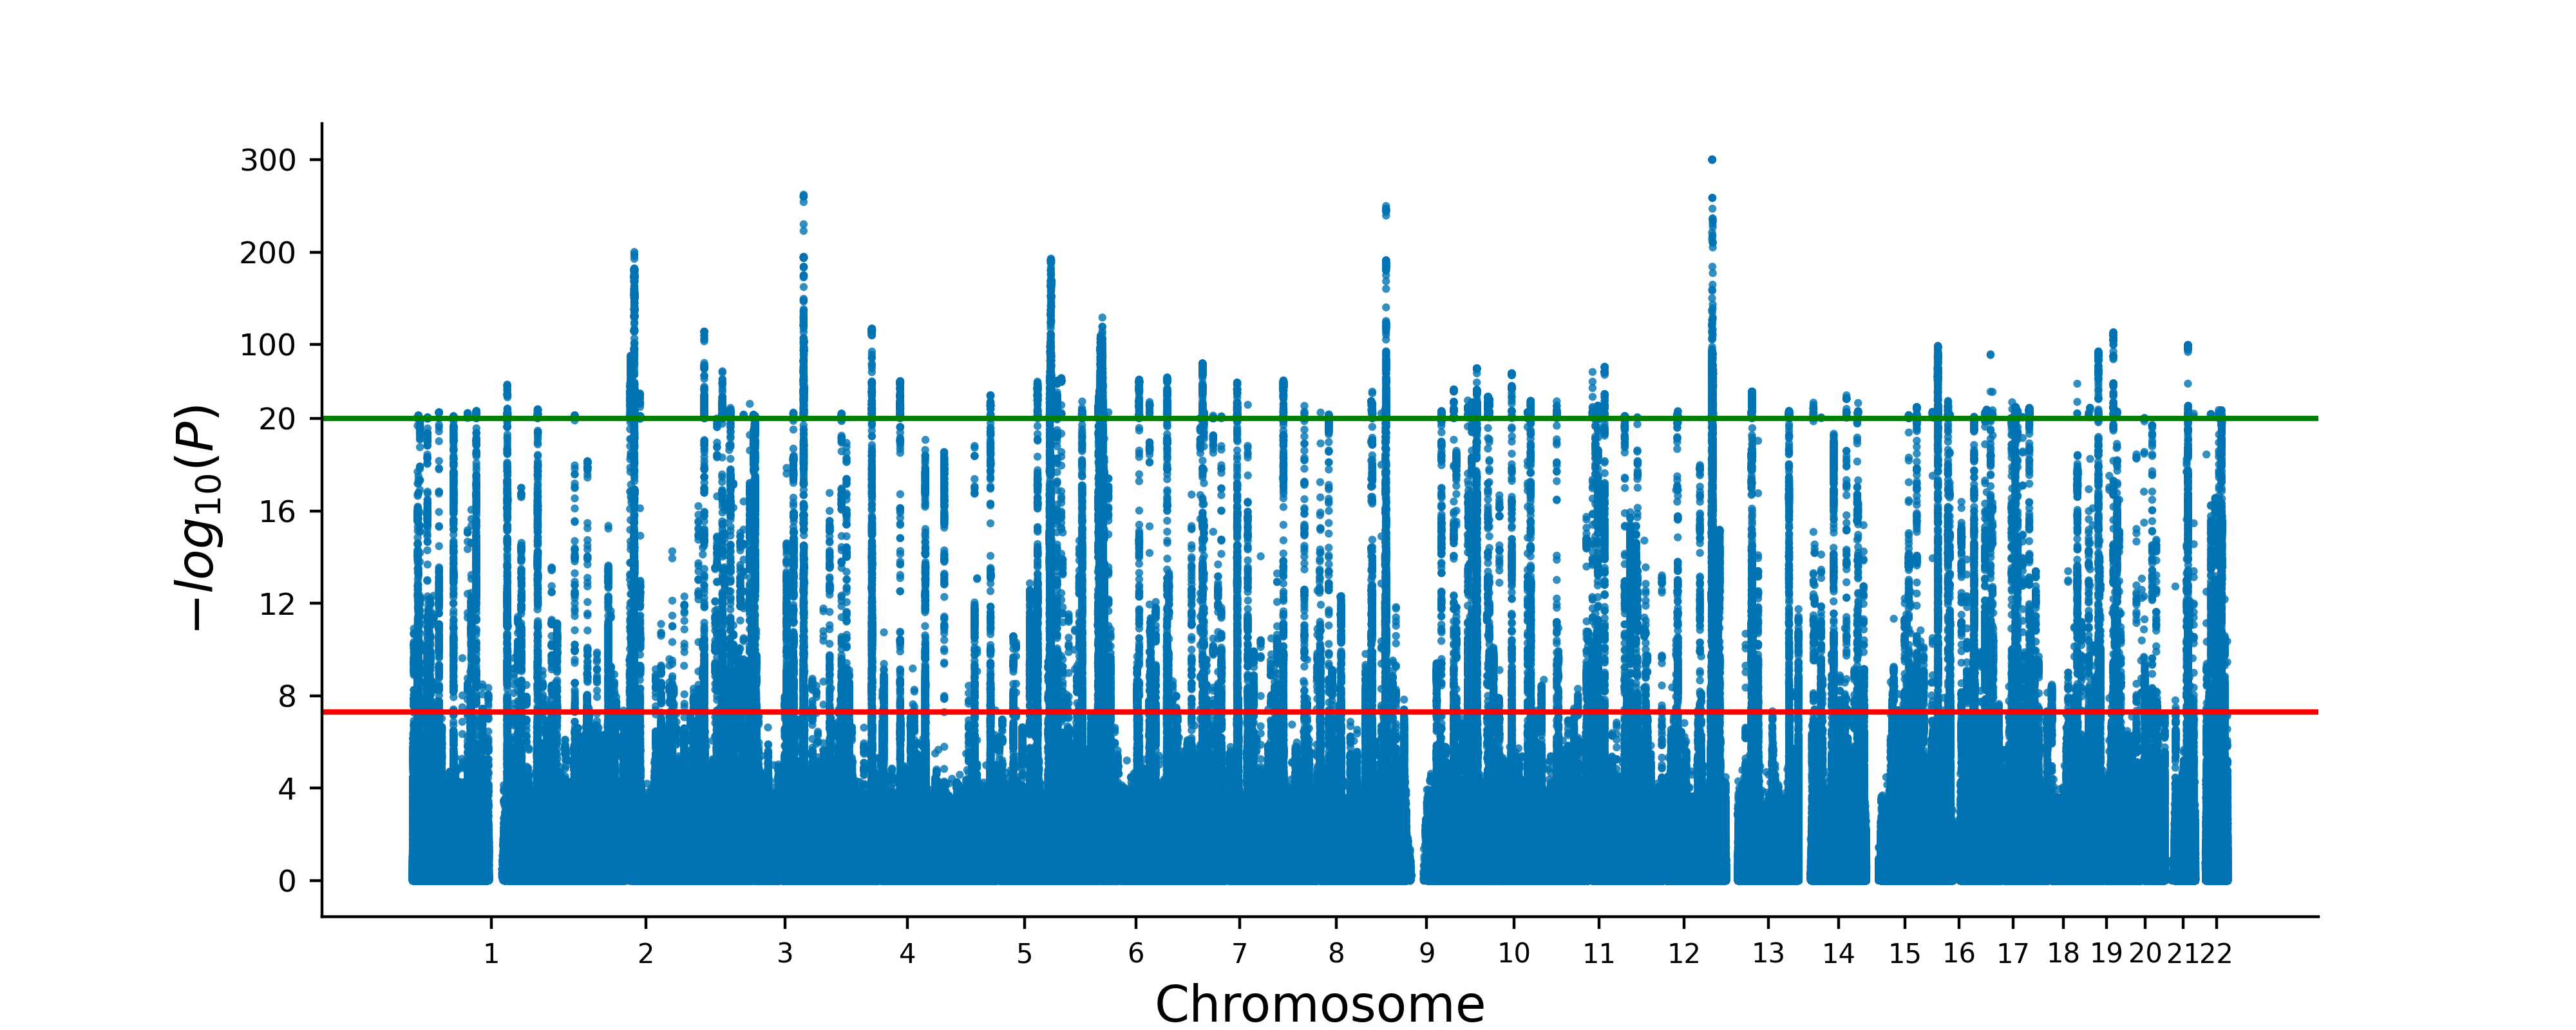
\includegraphics[width=\textwidth]{figures/manhattan_quant/qd_Eosinophill_count.sumstats.gz.png}
    \caption{}
    \end{subfigure}%
    \begin{subfigure}{.5\textwidth}
    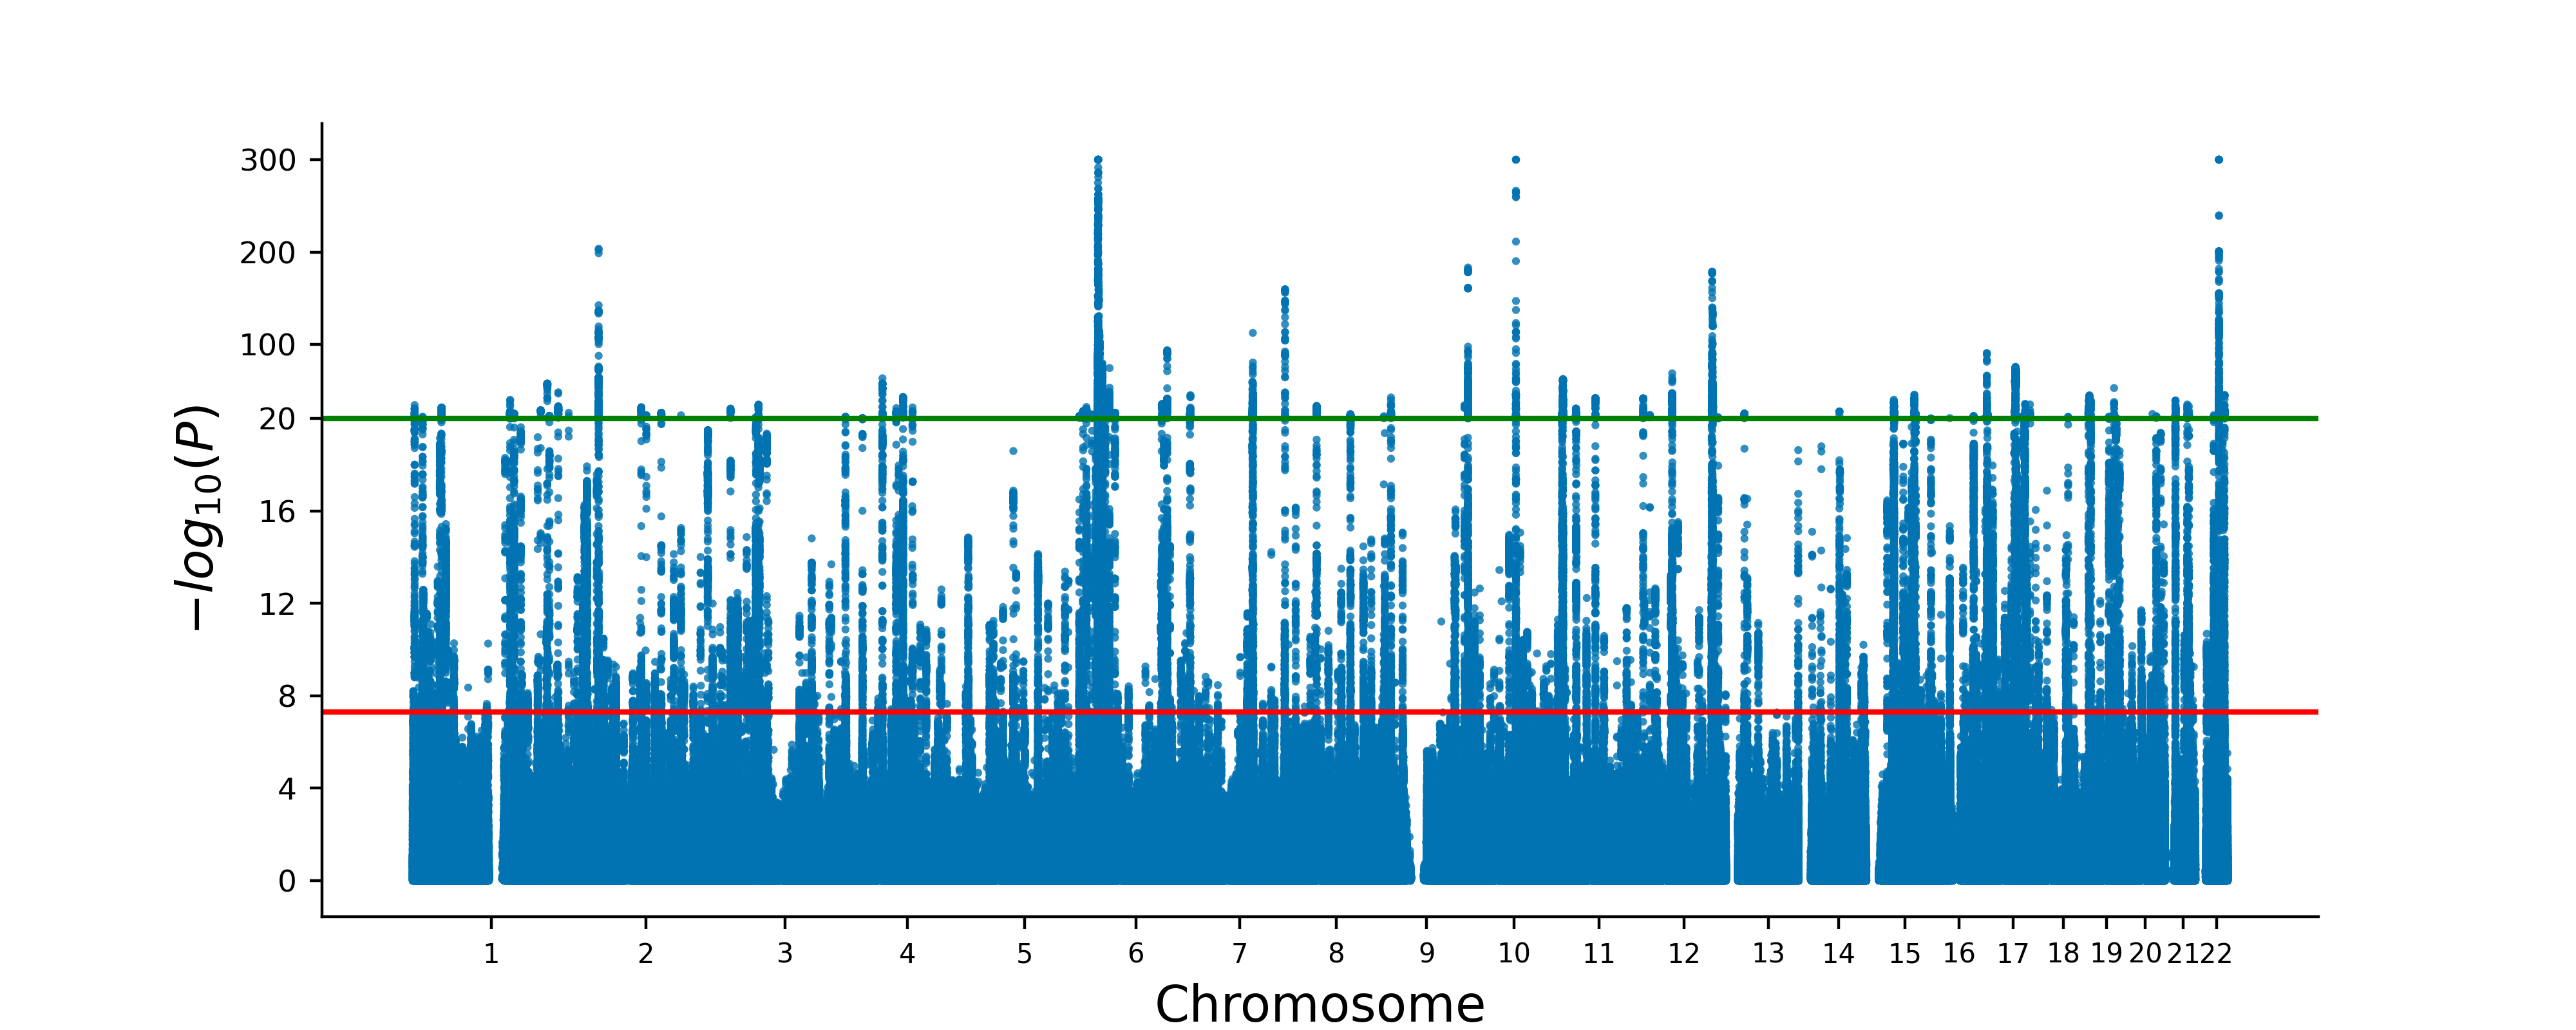
\includegraphics[width=\textwidth]{figures/manhattan_quant/qd_Haemoglobin_concentration.sumstats.gz.png}
    \caption{}
    \end{subfigure}
    \caption{\textbf{Manhattan plots for two quantitative traits.}
    %
    (a) Eosinophil count (RHE-me $h^2 = 0.213$) and (b) Haemoglobin concentration (RHE-mc $h^2 = 0.158$).
    %
    ${\sim}13.3$ million variants were tested.
    %
    Red lines indicate a genome-wide significance threshold of $ P = 5 \times 10^{-8}$ and the green line indicates $P = 1 \times 10^{-20}$.
    }
    \label{fig:qd_man_quant1}
\end{figure}

\begin{figure}[h!]
    \centering
    
\includegraphics[scale=0.425]{figures/manhattan_quant/legend.png}
    \begin{subfigure}{.5\textwidth}
    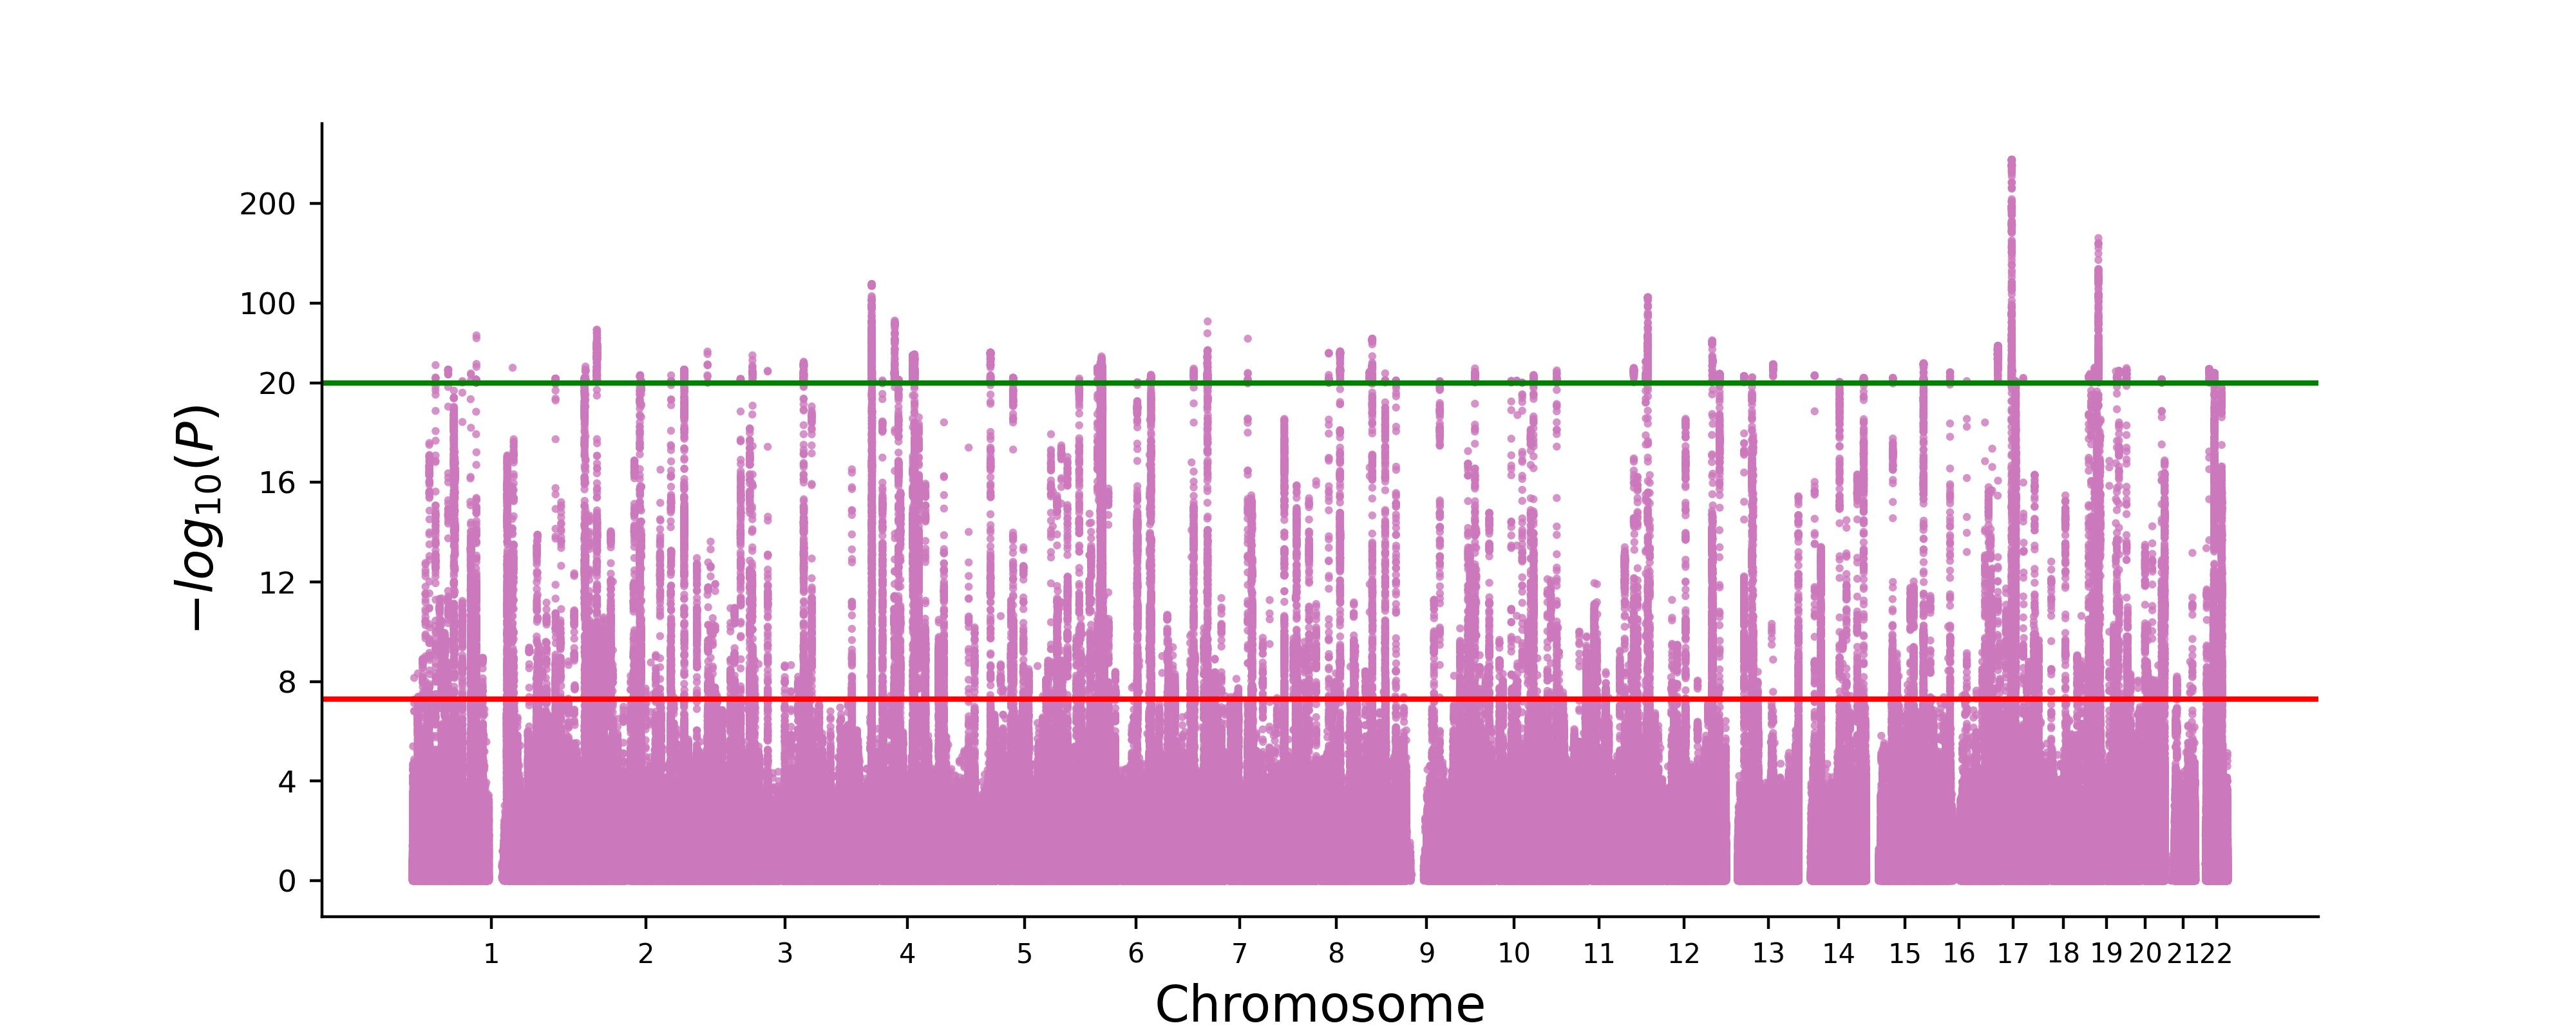
\includegraphics[width=\textwidth]{figures/manhattan_quant/imputed_fastgwa8.png}
    \end{subfigure}%
    \begin{subfigure}{.5\textwidth}
    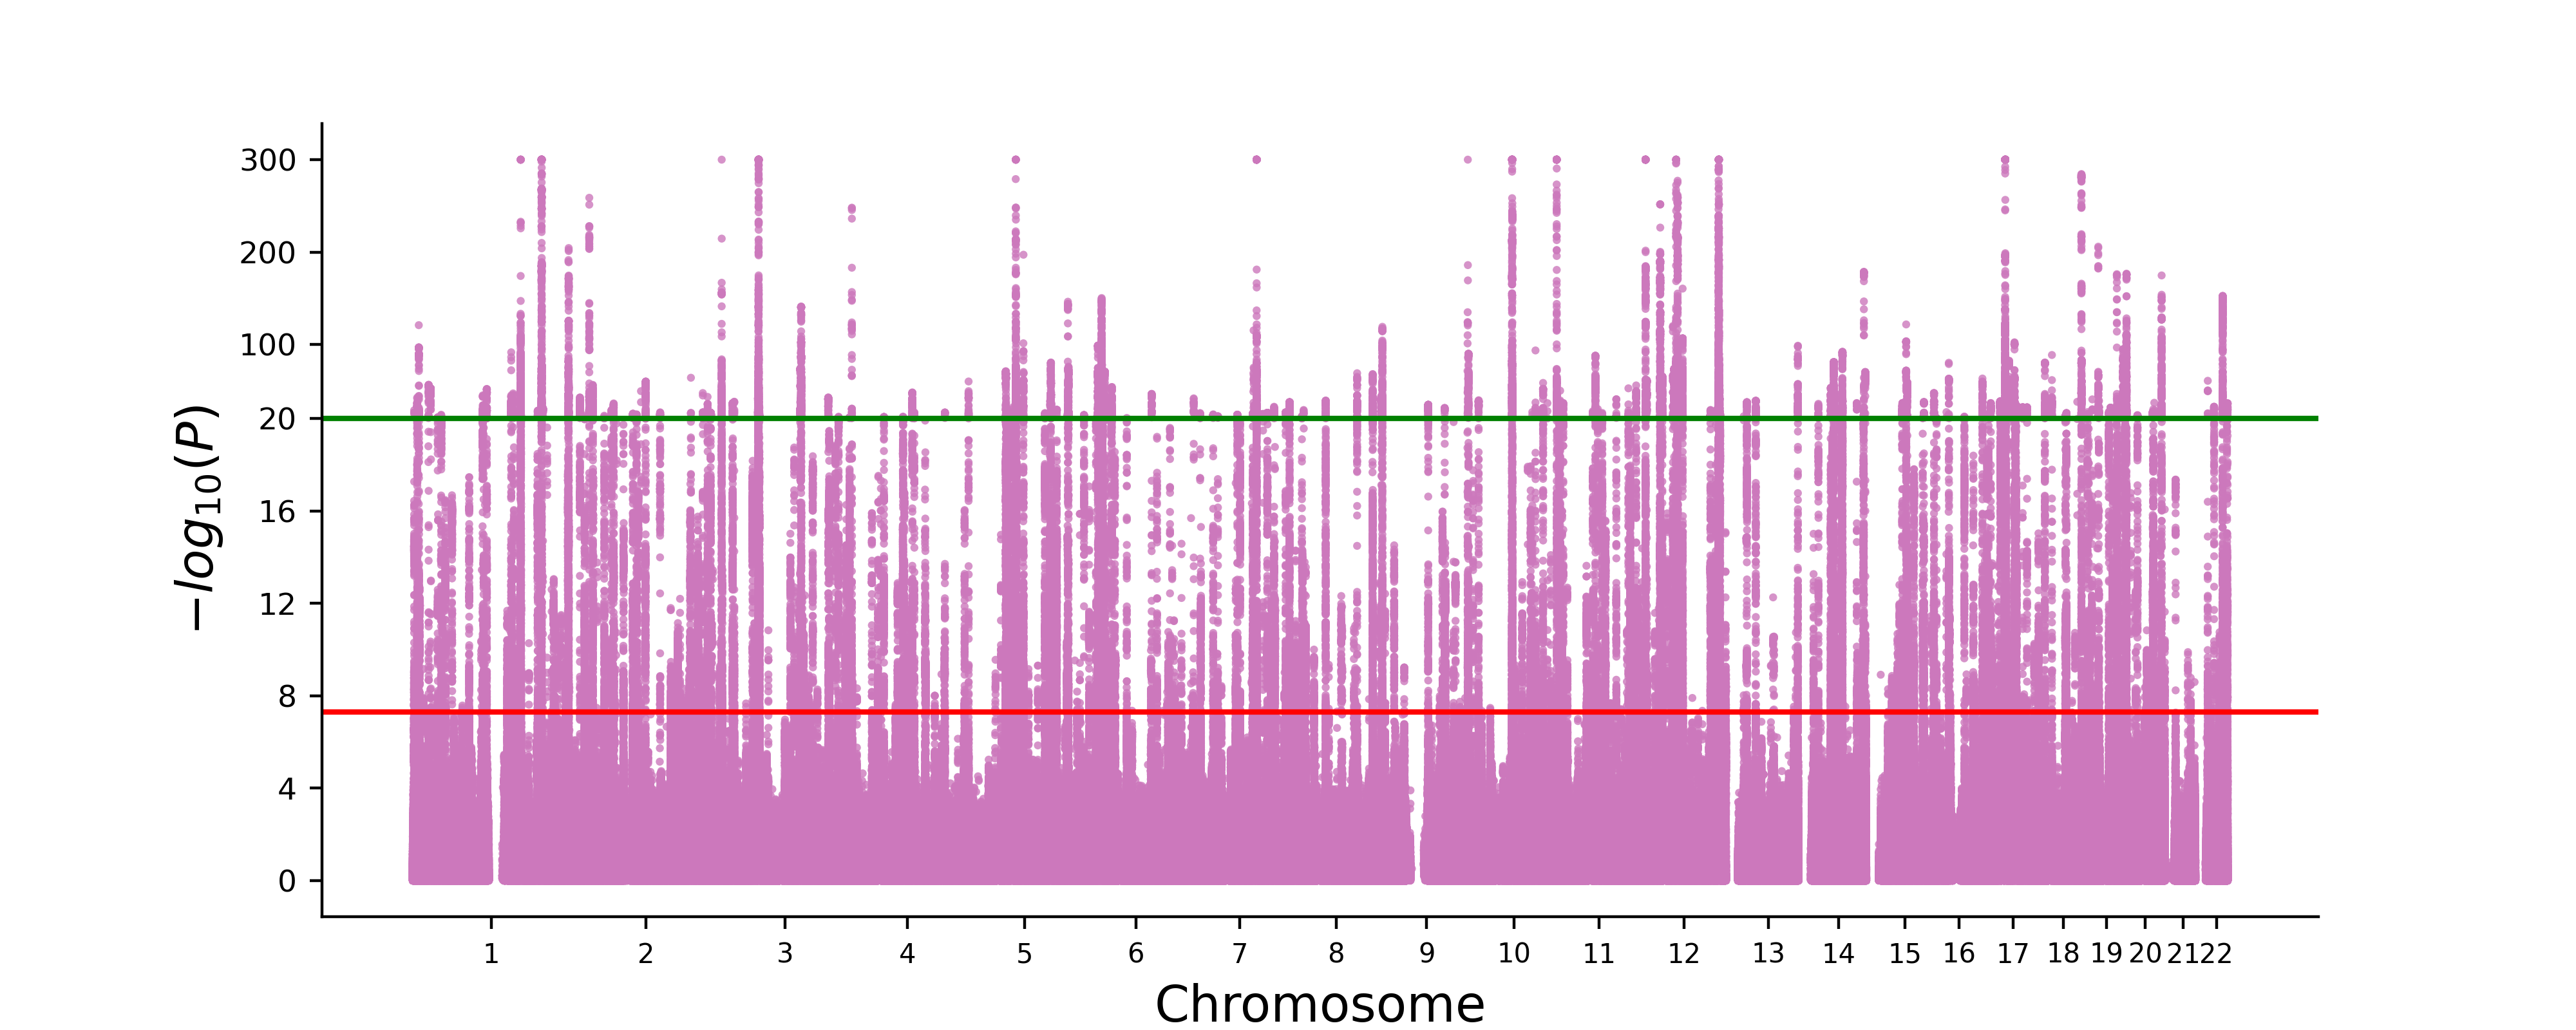
\includegraphics[width=\textwidth]{figures/manhattan_quant/imputed_fastgwa12.png}
    \end{subfigure}
    \begin{subfigure}{.5\textwidth}
    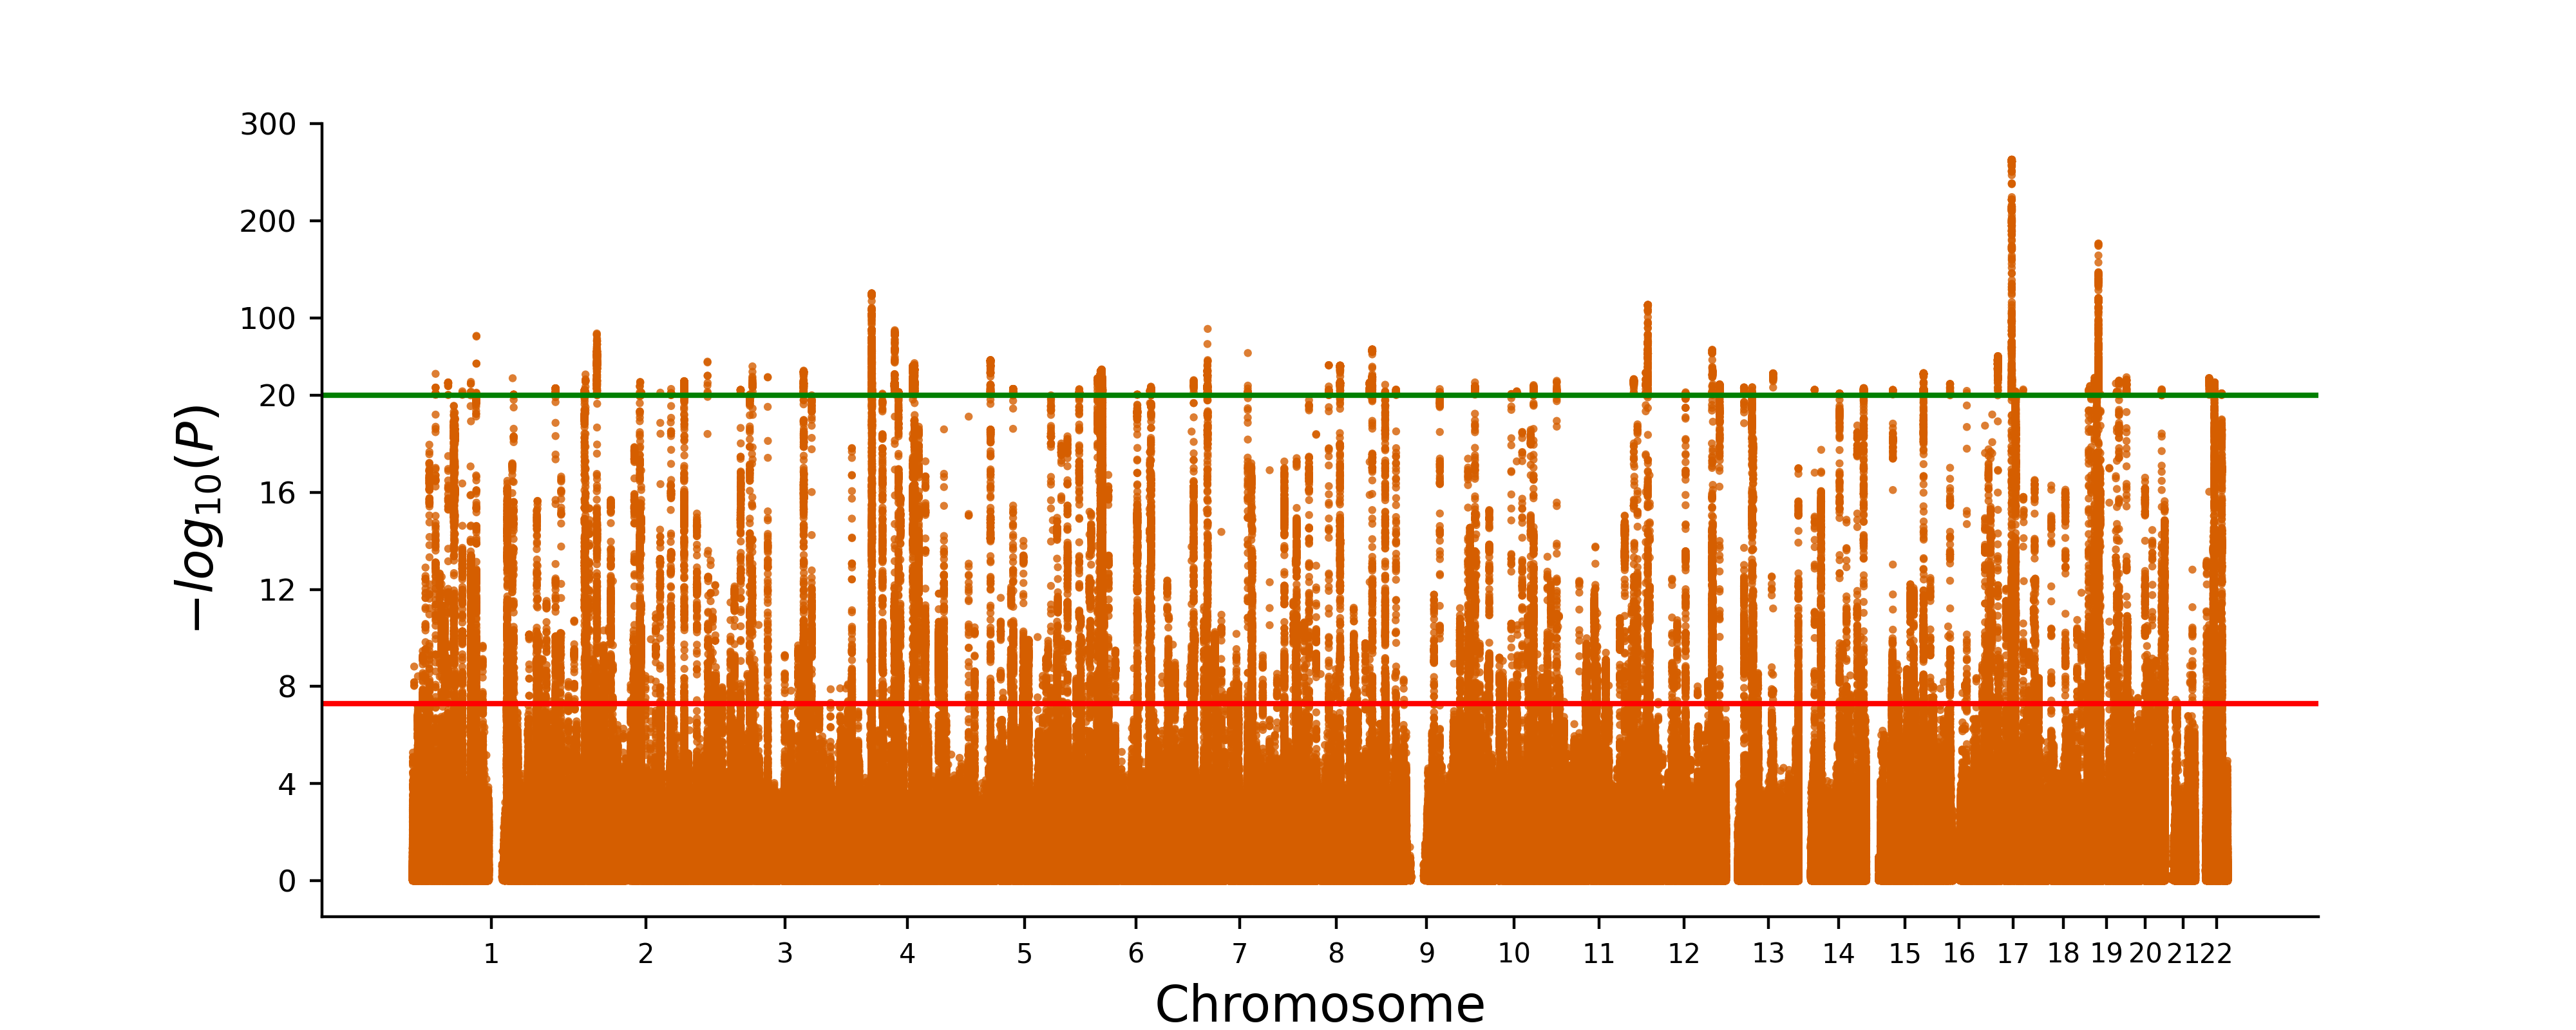
\includegraphics[width=\textwidth]{figures/manhattan_quant/regenie_400k_Lymphocyte_percentage.regenie.png}
    \end{subfigure}%
    \begin{subfigure}{.5\textwidth}
    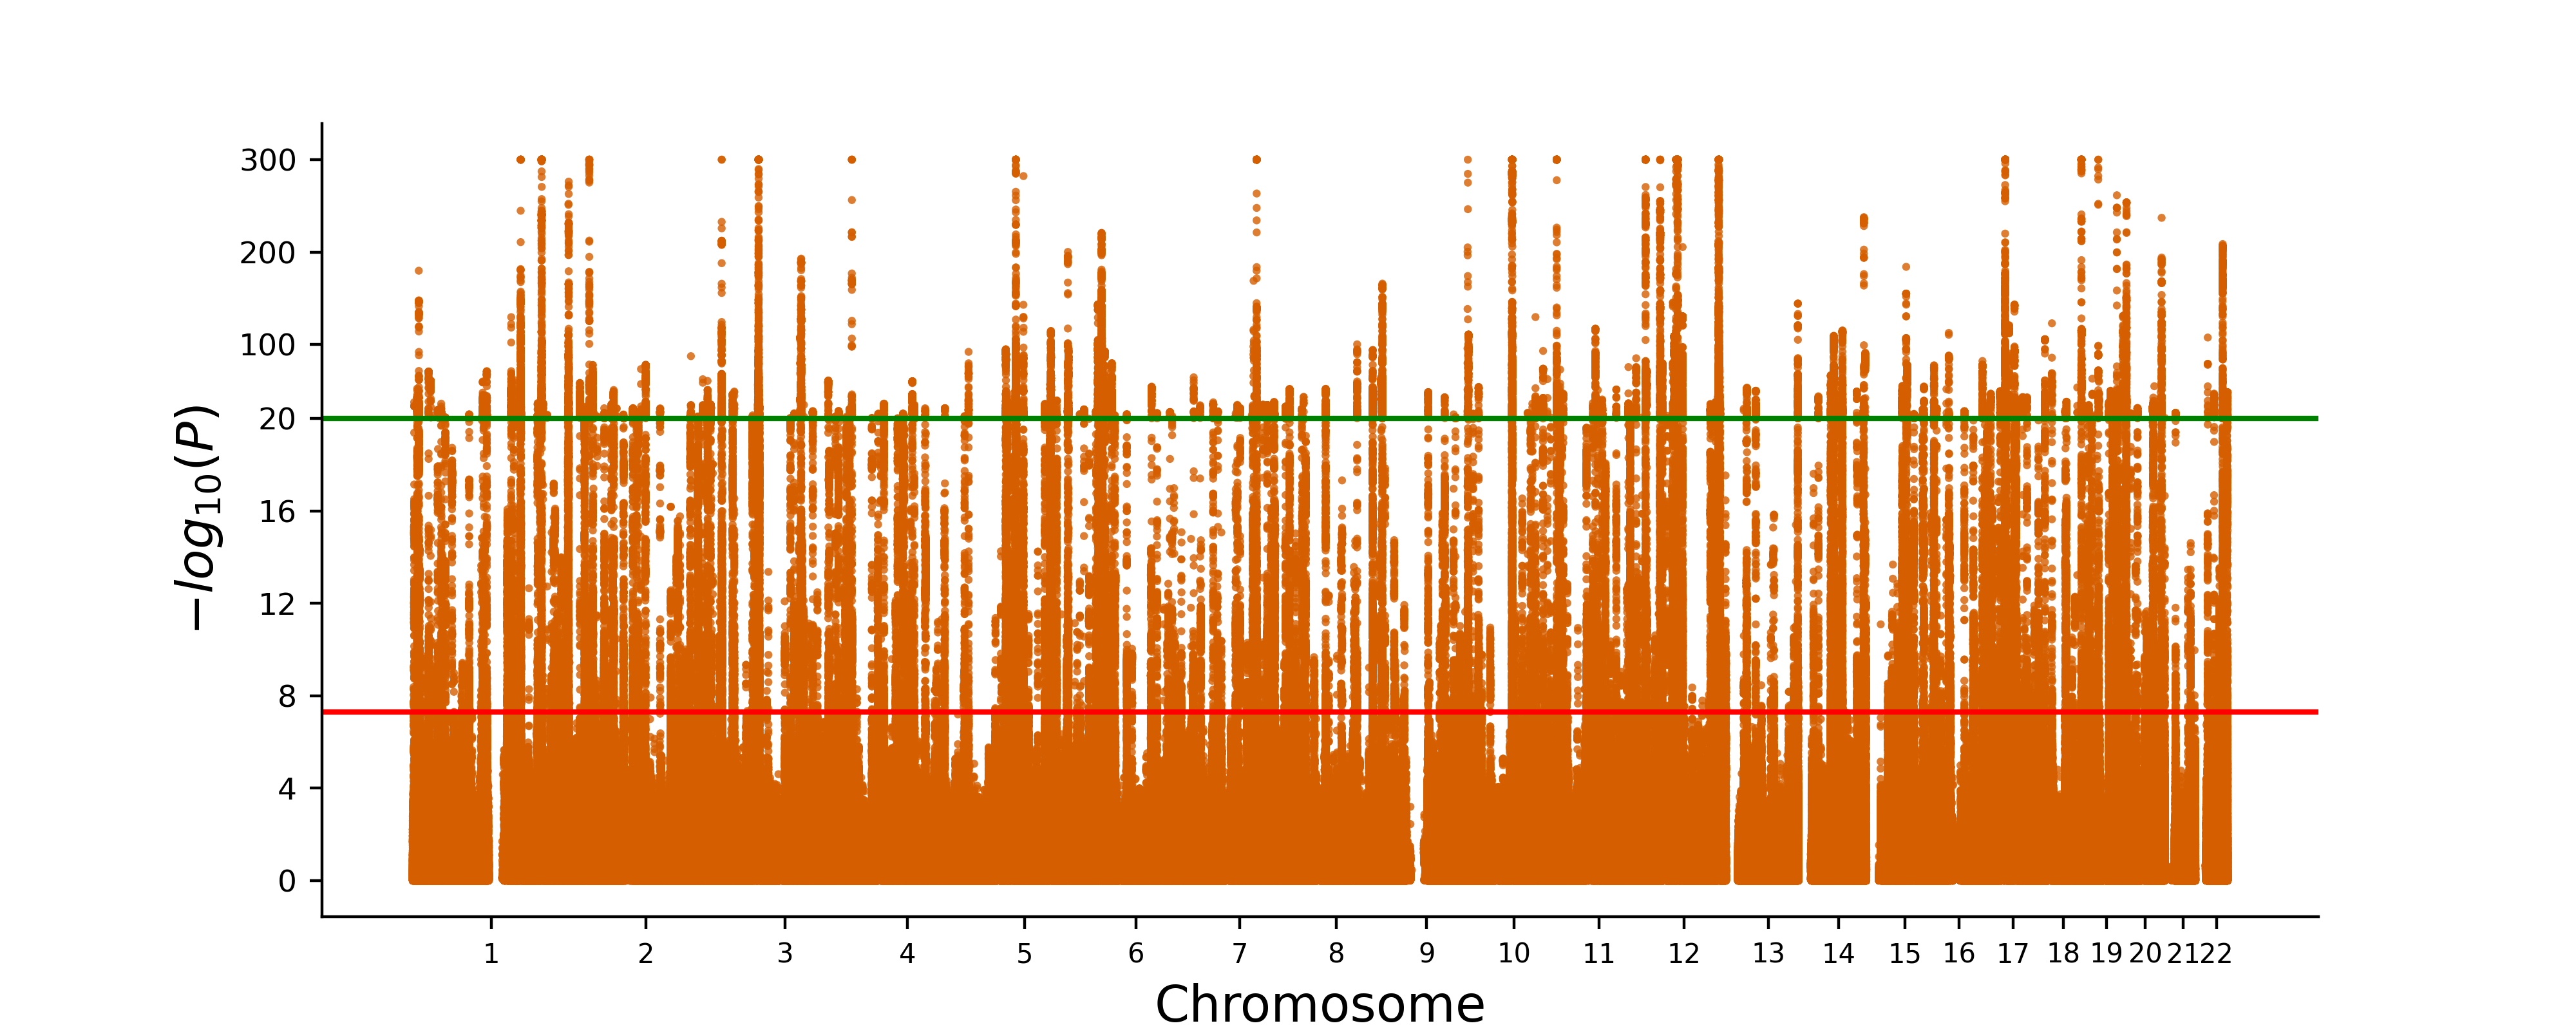
\includegraphics[width=\textwidth]{figures/manhattan_quant/regenie_400k_Mean_platelet_thrombocyte_volume.regenie.png}
    \end{subfigure}
    \begin{subfigure}{.5\textwidth}
    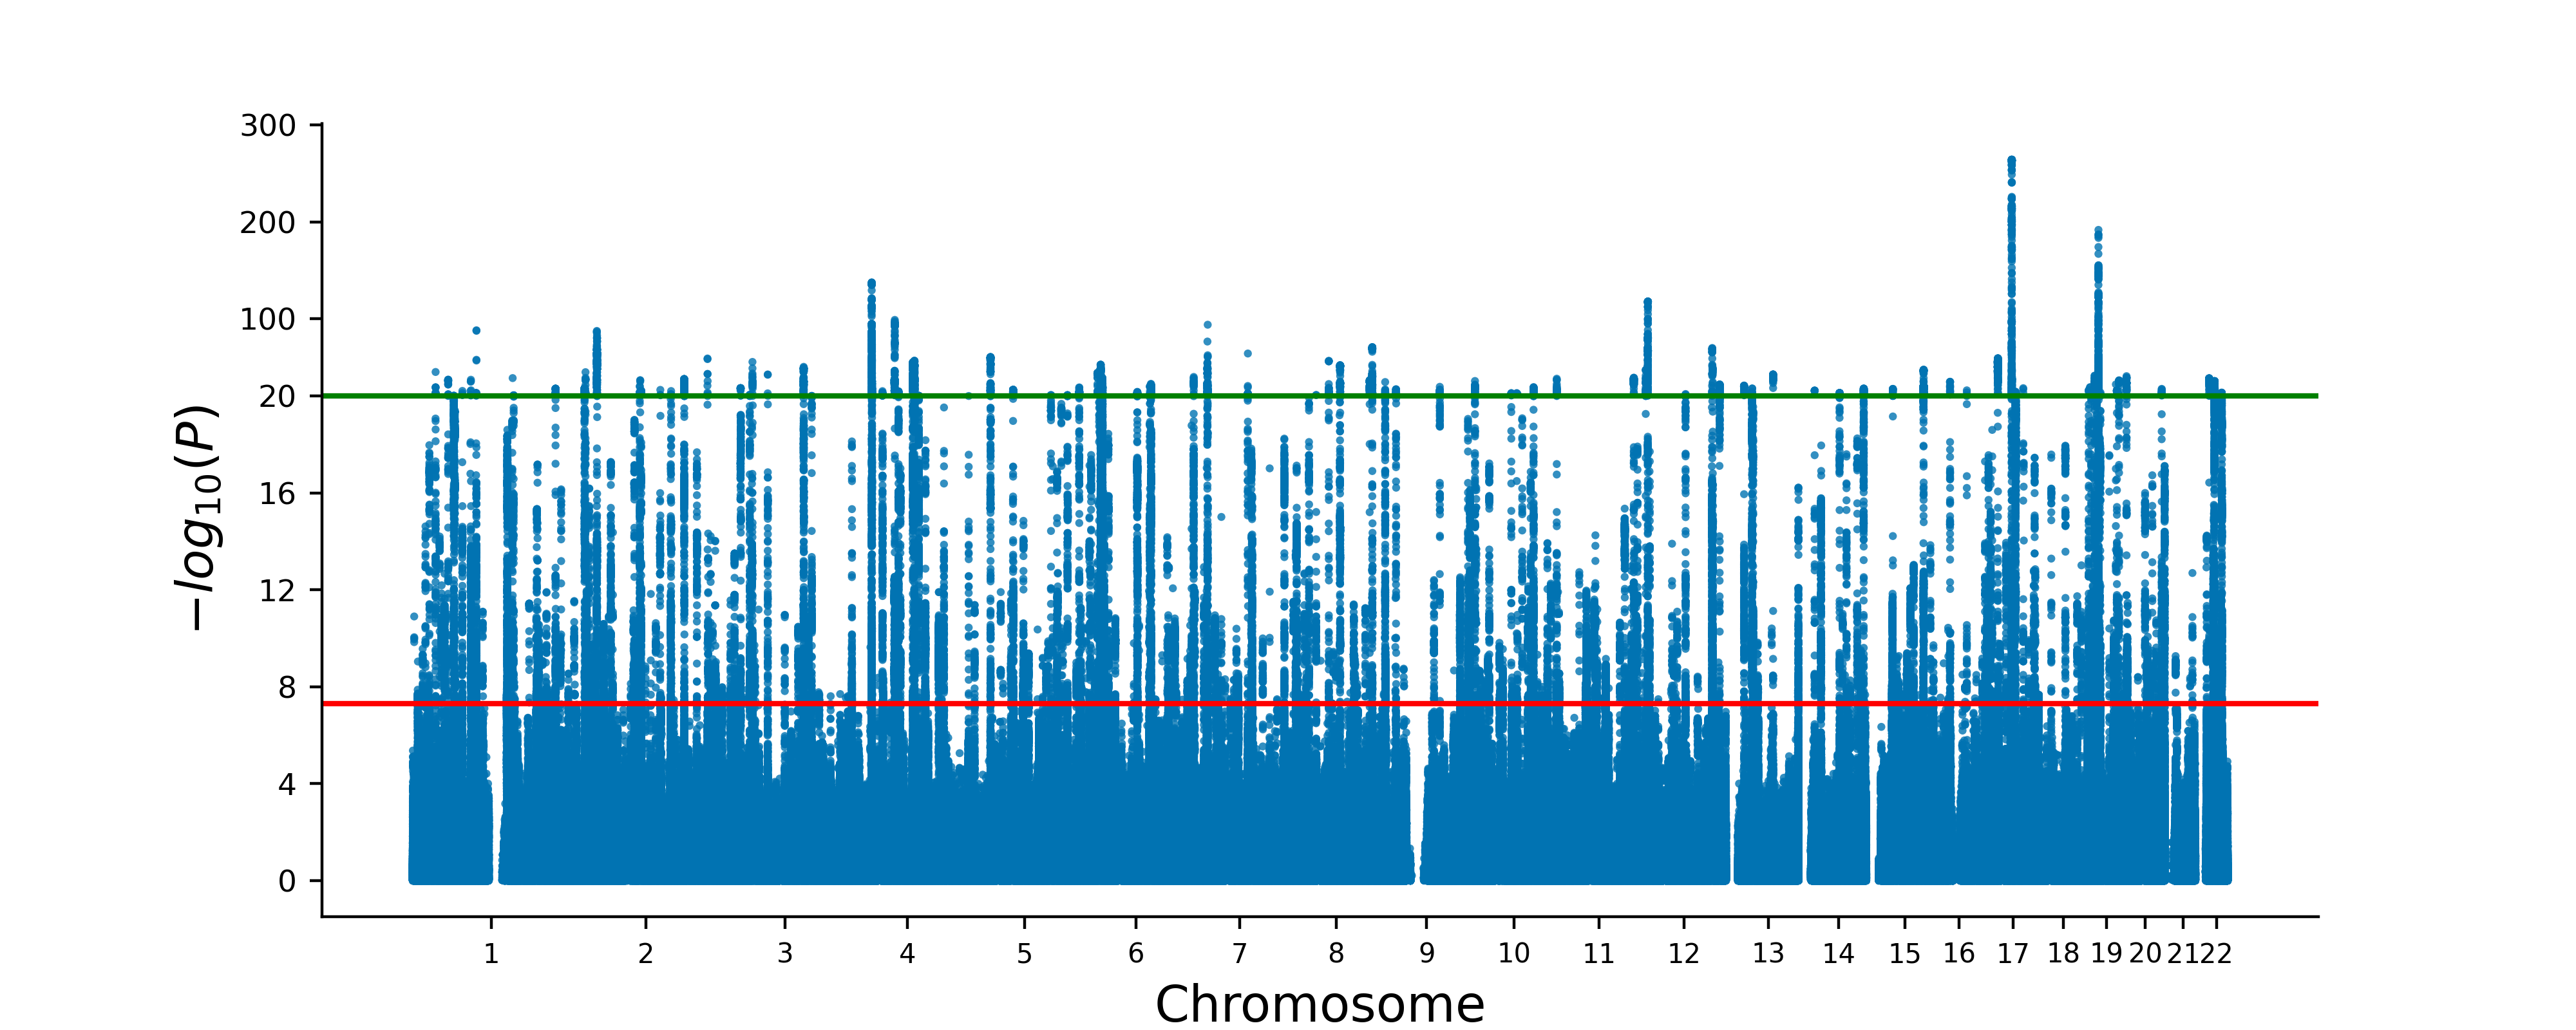
\includegraphics[width=\textwidth]{figures/manhattan_quant/qd_Lymphocyte_percentage.sumstats.gz.png}
    \caption{}
    \end{subfigure}%
    \begin{subfigure}{.5\textwidth}
    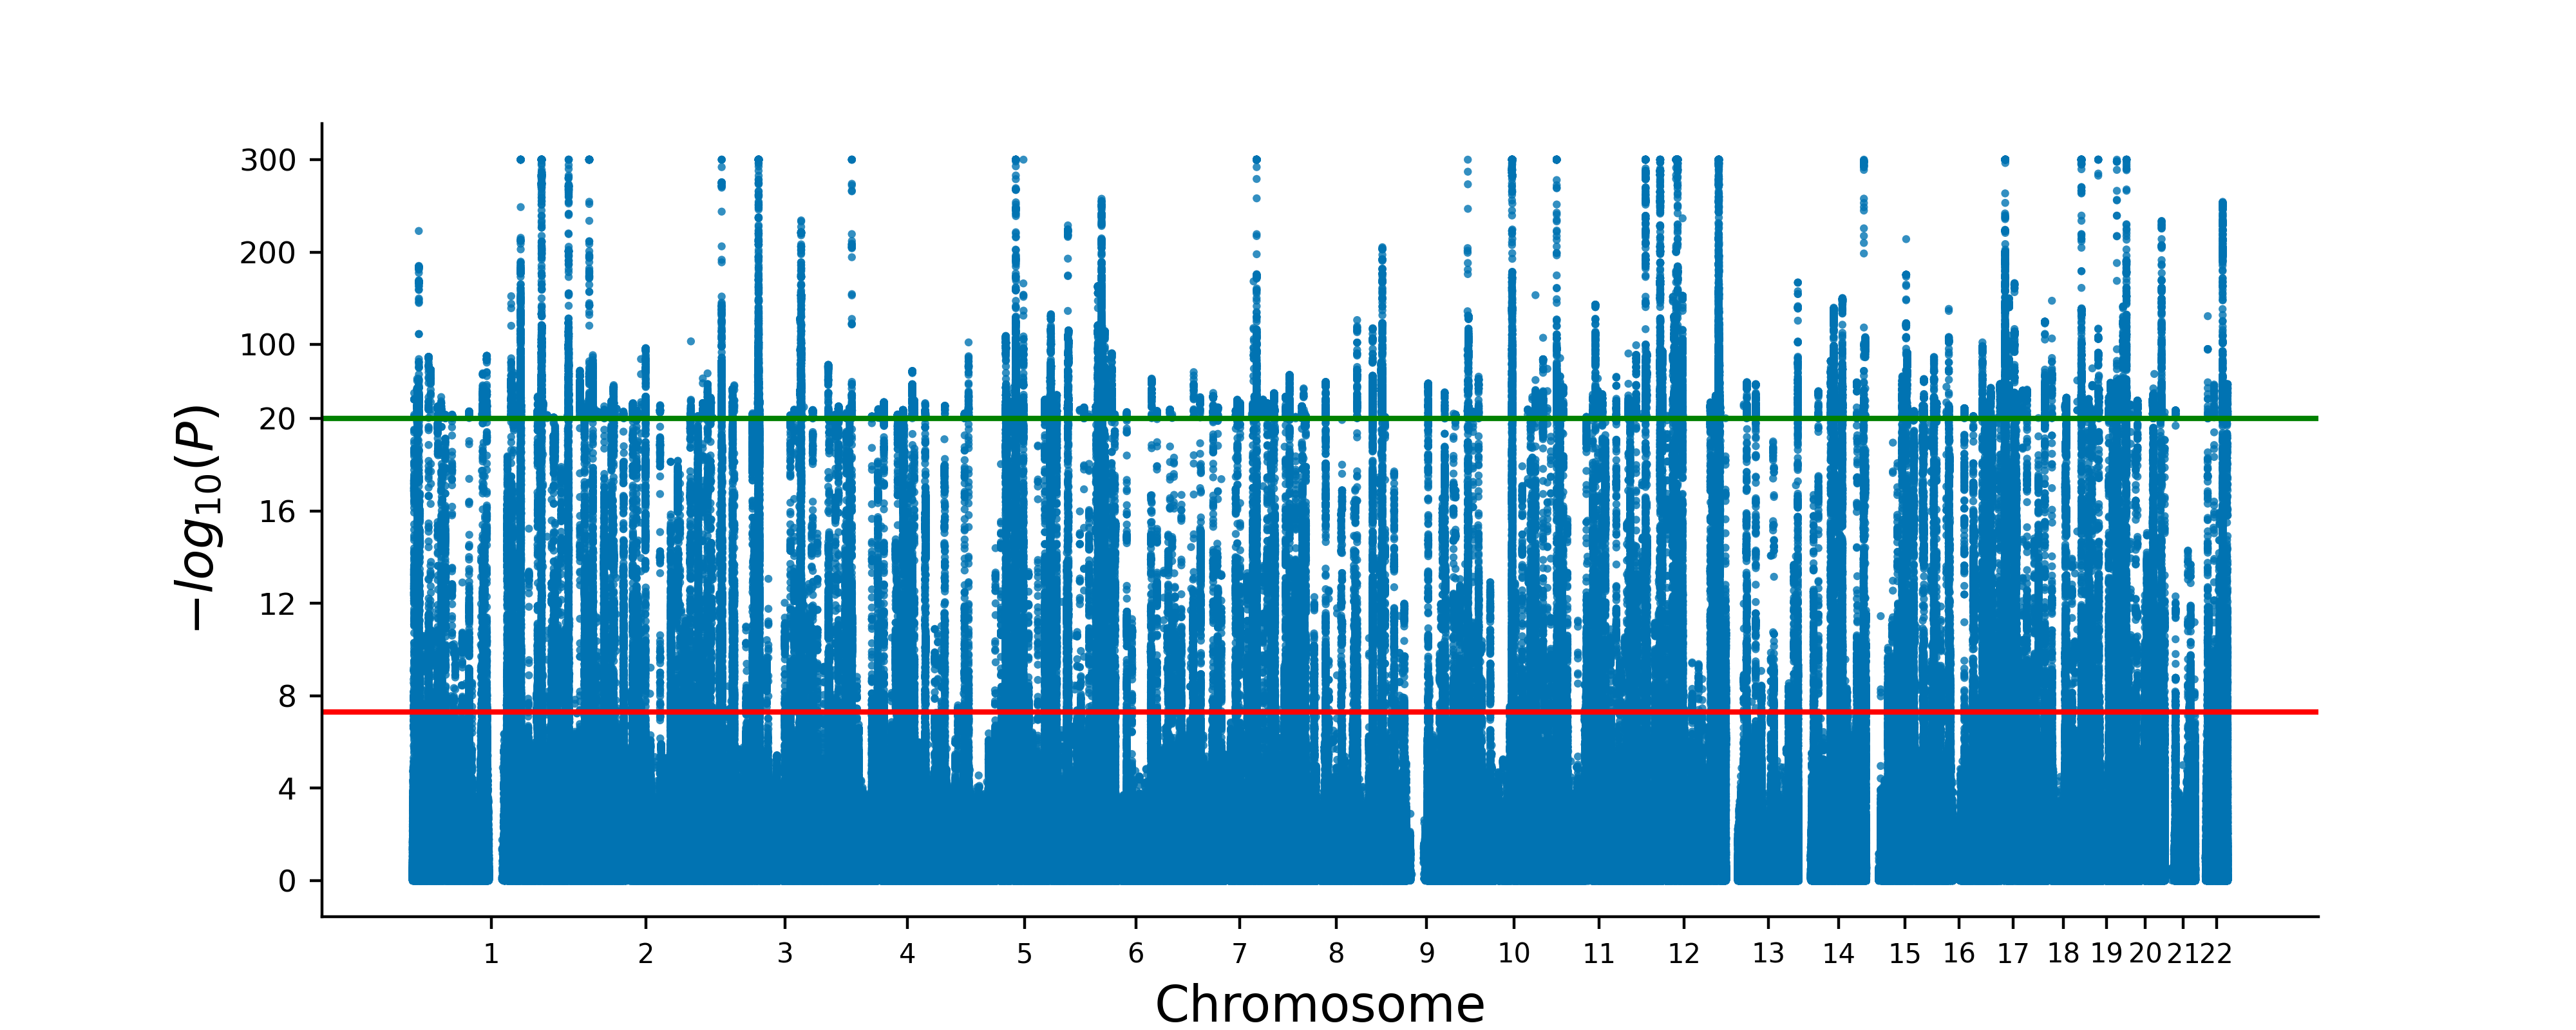
\includegraphics[width=\textwidth]{figures/manhattan_quant/qd_Mean_platelet_thrombocyte_volume.sumstats.gz.png}
    \caption{}
    \end{subfigure}
    \caption{\textbf{Manhattan plots for two quantitative traits.}
    %
    (a) Lymphocyte percentage (RHE-mc $h^2 = 0.196$) and (b) Mean platelet volume (RHE-mc $h^2 = 0.448$).
    %
    ${\sim}13.3$ million variants were tested.
    %
    Red lines indicate a genome-wide significance threshold of $ P = 5 \times 10^{-8}$ and the green line indicates $P = 1 \times 10^{-20}$.
    }
    \label{fig:qd_man_quant2}
\end{figure}


\clearpage

\section{Additional tables}
\label{sec:additional_tables}

\begin{longtable}{|l|c|c|c|}
\caption{\textbf{Ancient samples built in the genealogy.} Ancient sample IDs, sampling age (in years), country of origin and genomic coverage} \\
\hline
\textbf{ID} & \textbf{Date} & \textbf{Country} & \textbf{Coverage} \\
\hline
\endfirsthead

\caption{\textit{(Continued)}} \\
\hline
\textbf{ID} & \textbf{Date} & \textbf{Country} & \textbf{Coverage} \\
\hline
\endhead

\hline
\multicolumn{4}{r}{\textit{Continued on next page}} \\
\endfoot

\hline
\endlastfoot

AltaiNeandertal & 110,450 & Russia & 52.0 \\ \hline
Vindija & 41,950 & Croatia & 30.0 \\ \hline
Chagyrskaya & 80,000 & Russia & 27.0 \\ \hline
Denisova & 63,900 & Russia & 31.0 \\ \hline
WC1 & 9,219 & Iran & 10.4 \\ \hline
PB675 & 5,416 & Ireland & 15.9 \\ \hline
JP14 & 5,497 & Ireland & 16.6 \\ \hline
SRA62 & 5,979 & Ireland & 13.2 \\ \hline
rath1 & 3,906 & Ireland & 11.6 \\ \hline
bally & 5,132 & Ireland & 11.3 \\ \hline
Yamnaya & 4,890 & Kazakhstan & 25.2 \\ \hline
BOT2016 & 5,450 & Kazakhstan & 13.6 \\ \hline
Ust\_Ishim & 45,020 & Russia & 42.0 \\ \hline
SF12 & 8,895 & Sweden & 65.2 \\ \hline
KH150622 & 3,350 & Germany & 18.2 \\ \hline
KH150623 & 3,350 & Germany & 17.1 \\ \hline
KH150620 & 3,350 & Germany & 16.3 \\ \hline
KK1 & 9,678 & Georgia & 11.3 \\ \hline
I0018 & 7,140 & Germany & 19.0 \\ \hline
I0001 & 8,025 & Luxembourg & 20.1 \\ \hline
I10871 & 7,890 & Cameroon & 18.5 \\ \hline
I5950 & 4,472 & Ethiopia & 11.3 \\ \hline
Klein7 & 7,122 & Austria & 11.3 \\ \hline
Asp6 & 7,524.5 & Austria & 12.1 \\ \hline
Ess7 & 6,975 & Germany & 12.3 \\ \hline
Herx & 7,078.5 & Germany & 11.5 \\ \hline
Dil16 & 7,116.5 & Germany & 10.6 \\ \hline
Nea2 & 8,098 & Greece & 12.5 \\ \hline
Nea3 & 8,183.5 & Greece & 11.6 \\ \hline
VC3-2 & 7,495.5 & Serbia & 11.2 \\ \hline
STAR1 & 7,532.5 & Serbia & 10.6 \\ \hline
LEPE52 & 7,812 & Serbia & 12.4 \\ \hline
LEPE48 & 7,939.5 & Serbia & 10.9 \\ \hline
VLASA7 & 8,552 & Serbia & 15.2 \\ \hline
VLASA32 & 9,604.5 & Serbia & 12.7 \\ \hline
Bar25 & 8,294.5 & Turkey & 12.7 \\ \hline
AKT16 & 8,547.5 & Turkey & 12.3 \\ \hline
USR1 & 11,435 & USA & 17.0 \\ \hline
Sumidouro5 & 10,405 & Brazil & 13.6 \\ \hline
Lovelock3 & 627 & USA & 18.1 \\ \hline
Lovelock2 & 1,880 & USA & 14.4 \\ \hline
AHUR\_2064 & 10,970 & USA & 17.9 \\ \hline
Anzick & 12,649 & USA & 14.0 \\ \hline
new001 & 418 & South Africa & 11.1 \\ \hline
ela001 & 493 & South Africa & 10.5 \\ \hline
baa001 & 1,909 & South Africa & 12.9 \\ \hline
2H11 & 5,163 & France & 23.6 \\ \hline
2H10 & 5,166 & France & 13.8 \\ \hline
Kolyma1 & 9,786 & Russia & 15.0 \\ \hline
Yana1 & 31,950 & Russia & 24.3 \\ \hline
Sunghir3 & 34,093 & Russia & 12.0 \\ \hline
atp016 & 4,971 & Spain & 15.3 \\ \hline
atp002 & 4,746 & Spain & 11.3
\label{tab:gb_ancient_samples}
\end{longtable}

\begin{table}[h!]
\centering
\caption{\textbf{False positive rates (FPR) for FastGWA in quantitative trait simulations with up to 460,000 self-identified Europeans.} The table presents the FPR for FastGWA under various sample sizes, controlling for residual population stratification by adjusting the number of included principal components (PCs) or by omitting them entirely. The polygenicity of the simulated trait is fixed at 1\%. S.E. refers to the standard error, and * indicates a Bonferroni-significant t-test p-value. The significance threshold for the FPR was set at 0.005. Each simulation condition varied one of the following baseline parameters: sample size (N = 460k), ancestry differences explaining 5\% of phenotypic variance, and the use of 10 PCs to correct for stratification.}
\begin{tabular}{|l|c|c|c|}
\hline
\textbf{Condition} & \textbf{Mean FPR} & \textbf{S.E. FPR} & \textbf{t-test p-value} \\ \hline
\textbf{Varying sample sizes} & & & \\ 
N = 50k & 0.00503 & 2.99 x 10$^{-5}$ & 0.23 \\ 
N = 100k & 0.00514 & 4.35 x 10$^{-5}$ & 0.0009 \\ 
N = 460k & 0.00586 & 4.11 x 10$^{-5}$ & 8 x 10$^{-38}$ * \\ \hline
\textbf{Varying pop. stratification} & & & \\
5\% & 0.00586 & 4.11 x 10$^{-5}$ & 8 x 10$^{-38}$ * \\ 
0\% & 0.00509 & 2.94 x 10$^{-5}$ & 0.0019 \\ \hline
\textbf{Varying \#PCs} & & & \\ 
3 PCs & 0.01424 & 3.23 x 10$^{-4}$ & 2 x 10$^{-48}$ * \\ 
10 PCs & 0.00586 & 4.11 x 10$^{-5}$ & 8 x 10$^{-38}$ * \\ 
20 PCs & 0.00531 & 3.61 x 10$^{-5}$ & 1.8 x 10$^{-13}$ * \\ \hline
\end{tabular}
\label{tab:fgwa_fpr_sims}
\end{table}

\begin{longtable}{|c|c|c|c|}
\caption{\textbf{Quantitative traits analyzed.} Quantitative traits analyzed, including RHE-MC $h^2$ estimates and sample sizes (N).} \label{tab:ukb_qt_traits} \\
\hline
\textbf{UKBB ID} & \textbf{Phenotype} & \textbf{$h^2$} & \textbf{N}   \\
\hline
\endfirsthead
\caption{\textit{(Continued)}}\\
\hline
\textbf{UKBB ID} & \textbf{Phenotype} & \textbf{$h^2$} & \textbf{N}  \\
\hline
\endhead
\hline
\multicolumn{4}{r}{\textit{Continued on next page}} \\
\endfoot
\hline
\endlastfoot
30850 &  Testosterone & 0.03 & 355373 \\
1438 & Bread intake & 0.053 & 396396\\
874 & Duration of walks & 0.054 & 346657\\
30750 &  Glucose & 0.088 & 359138 \\
2217 & Age started wearing glasses & 0.092 & 349337\\
30710 &  Mean corp. haemoglobin conc. & 0.101 & 398336 \\
30810 &  Phosphate & 0.149 & 358861 \\
30790 &  LDL direct & 0.152 & 390888  \\
3064 & Peak expiratory flow (PEF) & 0.152 & 370024\\
30690 &  Cholesterol & 0.157 & 391567 \\
30760 &  Haemoglobin conc & 0.158 & 398342 \\
30020 &  Haematocrit \% & 0.161 & 398343 \\
46 & Hand grip strength (left) & 0.162 & 403800\\
47 & Hand grip strength (right) & 0.164 & 403850\\
30600 &  Albumin & 0.168 & 359528 \\
30670 &  Urea & 0.172 & 391307 \\
30680 &  Calcium & 0.177 & 359391 \\
30650 &  Asp-aminotransferase & 0.178 & 390183 \\
30860 &  Total protein & 0.188 & 359122 \\
4079 & Diastolic blood pressure & 0.188 & 379181\\
30640 &  Apolipoprotein B & 0.189 & 389718 \\
30200 &  Neutrophill \% & 0.19 & 397665 \\
4080 & Systolic blood pressure & 0.192 & 379174 \\
102 & Pulse rate & 0.194 & 379181 \\
30120 &  Lymphocyte \% & 0.196 & 397665 \\
30210 &  Creatinine & 0.198 & 391377  \\
30830 &  SHBG & 0.2 & 356165 \\
30880 &  Urate & 0.206 & 391102 \\
30630 &  Apolipoprotein A & 0.213 & 357411 \\
30730 &  Eosinophill count & 0.213 & 397661 \\
30180 &  Lipoprotein A & 0.22 & 312270 \\
30140 &  Neutrophill count & 0.22 & 397661  \\
30190 &  Monocyte \% & 0.221 & 397665 \\
30870 &  Triglycerides & 0.234 & 391260 \\
30740 &  Gamma glutamyltransferase & 0.24 & 391372 \\
30700 &  C-reactive protein & 0.241 & 390752 \\
20257 & Forced vital capacity (FVC) Z-score & 0.242 & 328403 \\
30030 &  Glycated haemoglobin & 0.245 & 391597  \\
30290 &  HDL cholesterol & 0.248 & 359370 \\
30150 &  Eosinophill \% & 0.251 & 397665 \\
30130 &  Monocyte count & 0.253 & 397661 \\
30780 &  Immature reticulocyte fraction & 0.26 & 391990 \\
30250 &  Reticulocyte count & 0.26 & 392210 \\
20256 & Forced expiratory volume (FEV1) Z-score & 0.263 & 328403\\
30070 &  Red blood cell distribution width & 0.264 & 398342  \\
30260 &  Mean reticulocyte vol & 0.266 & 392211 \\
30240 &  Reticulocyte \% & 0.267 & 392210 \\
20258 & FEV1/FVC ratio Z-score & 0.269 & 328403\\
30050 &  Lymphocyte count & 0.269 & 397661 \\
48 & Waist circumference & 0.277 & 404969\\
30010 &  Red blood cell count & 0.279 & 398343 \\
30610 &  Alkaline phosphatase & 0.279 & 391586 \\
30770 &  High light scatter reticulocyte count & 0.289 & 391989 \\
30280 &  IGF-1 & 0.29 & 389525 \\
30270 &  Mean sphered cell vol & 0.293 & 391990 \\
23115 & Leg fat \% (left) & 0.294 & 399130\\
23111 & Leg fat \% (right) & 0.294 & 399151\\
30110 &  Platelet distribution width & 0.296 & 398153 \\
23127 & Trunk fat \% & 0.302 & 398940\\
23119 & Arm fat \% (right) & 0.302 & 399098\\
23123 & Arm fat \% (left) & 0.305 & 399037\\
30300 &  High light scatter reticulocyte \% & 0.306 & 391990 \\
23099 & Body fat \% & 0.310 & 398955\\
49 & Hip circumference & 0.318 & 404972\\
30090 &  Platelet crit & 0.326 & 398154 \\
30840 &  Total bilirubin & 0.327 & 389995 \\
23110 & Impedance of arm (left) & 0.331 & 399149\\
23109 & Impedance of arm (right) & 0.331 & 399133 \\
23128 & Trunk fat mass & 0.331 & 398918 \\
21001 & Body mass index (BMI) & 0.348 & 405010\\
23106 & Impedance of whole body & 0.367 & 399144 \\
30080 &  Platelet count & 0.373 & 398339   \\
21002 & Weight & 0.381 & 405018 \\
30040 &  Mean corp. vol & 0.414 & 398342  \\
23105 & Basal metabolic rate & 0.419 & 399169\\
23102 & Whole body water mass & 0.428 & 399179 \\
30060 &  Mean corp. haemoglobin & 0.432 & 398339 \\
30100 &  Mean platelet vol & 0.448 & 398334 \\
50 & Standing height & 0.745 & 405035 \\
\end{longtable}

\begin{longtable}{|c|c|c|c|}
\caption{\textbf{Self-reported disease traits analyzed.} Self-reported disease traits analyzed, including their disease code and prevalence.} \label{tab:ukb_bt_traits}
\\
\hline
\textbf{UKBB ID} & \textbf{Disease ID} & \textbf{Phenotype} & \textbf{Prevalence}   \\
\hline
\endfirsthead
\caption{\textit{(Continued)}}\\
\hline
\textbf{UKBB ID} & \textbf{Disease ID} & \textbf{Phenotype} & \textbf{Prevalence}   \\
\hline
\endhead
\hline
\multicolumn{4}{r}{\textit{Continued on next page}} \\
\endfoot
\hline
\endlastfoot
20002 & 1065 & Hypertension & 0.2740\\
20002 & 1473 & High cholestrol & 0.1400\\
20002 & 1111 & Asthma & 0.1190\\
20002 & 1465 & Osteoarthritis & 0.0946\\
20002 & 1387 & Hayfever & 0.0667\\
20002 & 1286 & Depression & 0.0649\\
20002 & 1138 & Gastric reflux & 0.0529\\
20002 & 1226 & Hypothyroidism & 0.0518\\
20002 & 1220 & Diabetes & 0.0421\\
20002 & 1265 & Migraine & 0.0343\\
20002 & 1074 & Angina & 0.0335\\
20002 & 1452 & Eczema & 0.0320\\
20002 & 1474 & Hiatus hernia & 0.0266\\
20002 & 1075 & Heart attack & 0.0247\\
20001 & 1002 & Breast cancer & 0.0241\\
20002 & 1094 & Deep venous thrombosis & 0.0210\\
20002 & 1162 & Cholelithiasis & 0.0188\\
20002 & 1294 & Back problem & 0.0183\\
20002 & 1396 & Enlarged prostate & 0.0183\\
20002 & 1309 & Osteoporosis & 0.0182\\
20002 & 1287 & Anxiety & 0.0182\\
20002 & 1351 & Uterine fibroids & 0.0170\\
20002 & 1538 & Arthritis nos & 0.0148\\
20002 & 1113 & Emphysema & 0.0142\\
20002 & 1458 & Diverticulitis & 0.0137\\
20002 & 1453 & Psoriasis & 0.0131\\
20002 & 1277 & Glaucoma & 0.0125\\
20001 & 1061 & Basal cell carcinoma & 0.0120\\
20001 & 1044 & Prostate cancer & 0.0097\\
20002 & 1223 & Type 2 diabetes & 0.0093\\
20002 & 1197 & Bladder stone & 0.0092\\
20002 & 1093 & Pulmonary embolism & 0.0088\\
20001 & 1059 & Malignant melanoma & 0.0087\\
20002 & 1225 & Hyperthyroidism & 0.0084\\
20002 & 1202 & Urinary frequency & 0.0069\\
20002 & 1353 & Vaginal prolapse & 0.0069\\
20002 & 1330 & Iron deficiency anaemia & 0.0065\\
20002 & 1463 & Ulcerative colitis & 0.0056\\
20002 & 1417 & Nasal polyps & 0.0050\\
20002 & 1295 & Joint disorder & 0.0049\\
20002 & 1456 & Coeliac disease & 0.0047\\
20002 & 1112 & Chronic obstructive airways disease & 0.0045\\
20002 & 1281 & Retinal detachment & 0.0041\\
20002 & 1123 & Sleep apnoea & 0.0038\\
20002 & 1331 & Pernicious anaemia & 0.0033\\
20002 & 1462 & Crohns disease & 0.0032\\
20002 & 1291 & Bipolar disorder & 0.0028\\
20002 & 1446 & Gout & 0.0026\\
20002 & 1661 & Vitiligo & 0.0005\\
20002 & 1430 & Hypopituitarism & 0.0004\\
\end{longtable}

\begin{footnotesize}
\begin{longtable}[h!]{|c|c|c|c|c|}
\caption{\textbf{Number of independent associated loci for quantitative traits.} Number of independent associated loci for quantitative traits after Plink clumping using summary statistics from FastGWA, Regenie, BOLT-LMM, and Quickdraws}\\
\hline
\textbf{Phenotype} & \textbf{FastGWA} & \textbf{Regenie} & \textbf{BOLT-MoG} & \textbf{Quickdraws}  \\
\hline
\endfirsthead
\caption{\textit{(Continued)}}\\
\hline
\textbf{Phenotype} & \textbf{FastGWA} & \textbf{Regenie} & \textbf{BOLT-MoG} & \textbf{Quickdraws}  \\
\hline
\endhead
\hline
\multicolumn{5}{r}{\textit{Continued on next page}} \\
\endfoot
\hline
\endlastfoot
Testosterone & 72 & 65 & 83 & 40 \\
Bread intake & 5 & 5 & 6 & 5 \\
Duration of walks & 0 & 0 & 1 & 0 \\
Glucose & 87 & 92 & 94 & 93 \\
Age started wearing glasses & 30 & 30 & 29 & 32 \\
Mean corp. haemoglobin conc. & 82 & 85 & 86 & 86 \\
Phosphate & 131 & 140 & 149 & 140 \\
LDL direct & 151 & 165 & 170 & 164 \\
Peak expiratory flow (PEF) & 82 & 85 & 83 & 85 \\
Cholesterol & 181 & 192 & 197 & 191 \\
Haemoglobin conc & 306 & 341 & 363 & 356 \\
Haematocrit \% & 276 & 305 & 317 & 316 \\
Hand grip strength (left) & 75 & 78 & 79 & 84 \\
Hand grip strength (right) & 76 & 89 & 91 & 91 \\
Albumin & 198 & 216 & 222 & 220 \\
Urea & 145 & 158 & 161 & 156 \\
Calcium & 178 & 196 & 205 & 198 \\
Asp-aminotransferase & 254 & 271 & 282 & 276 \\
Total protein & 250 & 277 & 296 & 290 \\
Diastolic blood pressure & 129 & 143 & 151 & 146 \\
Apolipoprotein B & 178 & 205 & 214 & 206 \\
Neutrophill \% & 266 & 290 & 304 & 306 \\
Systolic blood pressure & 150 & 157 & 162 & 154 \\
Pulse rate & 171 & 182 & 186 & 187 \\
Lymphocyte \% & 305 & 332 & 344 & 345 \\
Creatinine & 351 & 400 & 418 & 403 \\
SHBG & 275 & 334 & 348 & 328 \\
Urate & 228 & 262 & 272 & 265 \\
Apolipoprotein A & 252 & 306 & 319 & 294 \\
Eosinophill count & 299 & 334 & 345 & 356 \\
Lipoprotein A & 54 & 65 & 70 & 56 \\
Neutrophill count & 299 & 330 & 341 & 356 \\
Monocyte \% & 362 & 416 & 437 & 449 \\
Triglycerides & 234 & 287 & 288 & 294 \\
Gamma glutamyltransferase & 287 & 323 & 330 & 327 \\
C-reactive protein & 196 & 227 & 233 & 227 \\
Forced vital capacity (FVC) & 163 & 185 & 203 & 193 \\
Glycated haemoglobin & 345 & 400 & 418 & 408 \\
HDL cholesterol & 280 & 353 & 371 & 352 \\
Eosinophill \% & 375 & 430 & 463 & 461 \\
Monocyte count & 402 & 470 & 490 & 494 \\
Immature reticulocyte fraction & 234 & 258 & 262 & 264 \\
Reticulocyte count & 311 & 361 & 372 & 367 \\
Forced expiratory volume (FEV1) & 189 & 218 & 228 & 228 \\
Red blood cell distribution width & 368 & 423 & 443 & 425 \\
Mean reticulocyte vol & 395 & 439 & 463 & 460 \\
Reticulocyte \% & 307 & 353 & 363 & 361 \\
FEV1/FVC ratio & 272 & 301 & 323 & 307 \\
Lymphocyte count & 353 & 406 & 422 & 420 \\
Waist circumference & 186 & 206 & 214 & 212 \\
Alkaline phosphatase & 355 & 446 & 473 & 457 \\
Red blood cell count & 409 & 482 & 507 & 508 \\
High light scatter reticulocyte count & 325 & 373 & 393 & 390 \\
IGF-1 & 364 & 435 & 459 & 445 \\
Mean sphered cell vol & 378 & 430 & 456 & 456 \\
Leg fat \% (left) & 197 & 222 & 233 & 233 \\
Leg fat \% (right) & 204 & 220 & 229 & 235 \\
Platelet distribution width & 456 & 549 & 576 & 591 \\
Trunk fat \% & 197 & 224 & 238 & 237 \\
Arm fat \% (right) & 215 & 240 & 258 & 251 \\
Arm fat \% (left) & 206 & 242 & 256 & 246 \\
High light scatter reticulocyte \% & 324 & 369 & 398 & 399 \\
Body fat \% & 215 & 242 & 259 & 255 \\
Hip circumference & 255 & 292 & 308 & 306 \\
Platelet crit & 485 & 587 & 623 & 626 \\
Total bilirubin & 146 & 203 & 206 & 199 \\
Impedance of arm (left) & 257 & 292 & 309 & 307 \\
Impedance of arm (right) & 301 & 368 & 387 & 366 \\
Trunk fat mass & 302 & 367 & 384 & 373 \\
Body mass index (BMI) & 262 & 309 & 334 & 340 \\
Impedance of whole body & 354 & 451 & 488 & 452 \\
Platelet count & 539 & 670 & 720 & 721 \\
Weight & 329 & 398 & 428 & 423 \\
Mean corp. vol & 487 & 580 & 599 & 605 \\
Basal metabolic rate & 465 & 545 & 592 & 584 \\
Whole body water mass & 489 & 587 & 638 & 627 \\
Mean corp. haemoglobin & 429 & 538 & 562 & 569 \\
Mean platelet vol & 618 & 821 & 892 & 887 \\
Standing height & 1022 & 1327 & 1452 & 1674 \\
\hline
Total & 21,380 & 24,995 & 26,368 & 26,236
\label{tab:loci_qt}
\end{longtable}
\end{footnotesize}

\begin{footnotesize}
\begin{longtable}[h!]{|c|c|c|c|c|}
\caption{\textbf{Number of independent associated loci for binary traits.}
Number of independent associated loci for binary traits after Plink clumping using summary statistics from FastGWA, SAIGE, Regenie, and Quickdraws.
%
We excluded traits (enlarged prostate, prostate cancer, vaginal prolapse, and uterine fibroids) which led to matrix inversion errors or non-convergence of Firth logistic regression, or for which no associations were found using any method.}\\
\hline
\textbf{Phenotype} & \textbf{FastGWA} & \textbf{SAIGE} & \textbf{Regenie} & \textbf{Quickdraws}  \\
\hline
\endfirsthead
\caption{\textit{(Continued)}}\\
\hline
\textbf{Phenotype} & \textbf{FastGWA} & \textbf{SAIGE} & \textbf{Regenie} & \textbf{Quickdraws}  \\
\hline
\endhead
\hline
\multicolumn{5}{r}{\textit{Continued on next page}} \\
\endfoot
\hline
\endlastfoot
 Hypertension  & 155 & 156 & 170 & 172 \\
 High cholesterol  & 52 & 52 & 56 & 57 \\
 Asthma  & 65 & 65 & 63 & 63 \\
 Osteoarthritis  & 2 & 2 & 2 & 2 \\
 Hayfever  & 20 & 21 & 20 & 20 \\
 Depression  & 1 & 1 & 1 & 1 \\
 Gastric reflux  & 1 & 1 & 1 & 1 \\
 Hypothyroidism  & 80 & 81 & 81 & 84 \\
 Diabetes  & 36 & 36 & 36 & 38 \\
 Migraine  & 9 & 9 & 8 & 9 \\
 Angina  & 8 & 9 & 9 & 8 \\ 
 Eczema  & 13 & 13 & 13 & 13 \\
 Hiatus hernia  & 0 & 0 & 0 & 0 \\
 Heart attack  & 9 & 8 & 9 & 9 \\
 Breast cancer  & 11 & 11 & 11 & 11 \\
 Deep venous thrombosis  & 9 & 9 & 9 & 9 \\
 Cholelithiasis  & 11 & 11 & 12 & 11\\
 % Back problem  & 0 & 0 & 0 & 0 \\
 % Enlarged prostate  &  NA* & NA* & 5 & 5 \\
 Osteoporosis  & 8 & 8 & 9 & 8 \\
 % Anxiety  & 0 & 0 & 0 & 0 \\
 % Uterine fibroids  &  NA* & NA* & 5 & 5 \\
 % Arthritis nos  & 0 & 0 & 0 & 0 \\
 % Emphysema  & 0 & 0 & 0 & 0 \\
 Diverticulitis  & 1 & 1 & 1 & 1 \\
 Psoriasis  & 21 & 21 & 18 & 25 \\
 Glaucoma  & 6 & 6 & 6 & 6 \\
 Basal cell carcinoma  & 12 & 12 & 12 & 12 \\
 % Prostate cancer  &  NA* & NA* & 12 & 13 \\
 Type 2 diabetes  & 2 & 2 & 2 & 2 \\
 Bladder stone  & 1 & 1 & 1 & 1 \\
 Pulmonary embolism  & 5 & 5 & 5 & 6 \\
 Malignant melanoma  & 3 & 3 & 2 & 3 \\
 Hyperthyroidism  & 12 & 12 & 11 & 12 \\
 % urinary frequency  & 0 & 0 & 0 & 0 \\
 % Vaginal prolapse  &  NA & NA & 0 & 0 \\
 % Iron deficiency anaemia  & 0 & 0 & 0 & 0 \\
 Ulcerative colitis  & 8 & 8 & 8 & 8 \\
 Nasal polyps  & 5 & 5 & 6 & 6 \\
 % Joint disorder  & 0 & 0 & 0 & 0 \\
 Celiac disease  & 24 & 26 & 30 & 32 \\
 Chronic obstructive airways disease  & 1 & 1 & 0 & 1 \\
 % Retinal detachment  & 0 & 0 & 0 & 0 \\
 % Sleep apnoea  & 0 & 0 & 0 & 0  \\
 Pernicious anaemia  & 1 & 1 & 2 & 2  \\
 Crohns disease  & 2 & 2 & 2 & 3 \\
 % Bipolar disorder  &  NA & 0 & 0 & 0  \\
 % Gout  & 0 & 0 & 0 & 0 \\
 % Vitiligo  & 0 & 0 & 0 & 0 \\
 % Hypopituitarism  & 0 & 0 & 0 & 0 \\
\hline
 Total & 594 & 599 & 616 & 636
\label{tab:loci_bt}
\end{longtable}
\end{footnotesize}

\begin{table}[h!]
    \centering
    \caption{\textbf{Number of individual variants replicated using trait-specific summary statistics.}
    %
    Number of individual variants replicated using summary statistics for Crohn's disease \cite{jostins2012host}, Type 2 Diabetes \cite{diabetes2012large}, Celiac disease \cite{dubois2010multiple}, Depression \cite{nagel2018meta}, and Ulcerative Colitis \cite{de2017genome}.
    %
    We use a discovery threshold of $5 \times 10^{-8}$ and vary the replication threshold from $5 \times 10^{-2}$ to $5 \times 10^{-6}$, and compare summary statistics from FastGWA, Regenie, and Quickdraws. }
    \resizebox{\textwidth}{!}{
    \begin{tabular}{|c|c|cc|cc|cc|}
    \hline
    Phenotype & Method & \multicolumn{2}{c}{Repl. thresh. $=5 \times 10^{-2}$} \vline & \multicolumn{2}{c}{Repl. thresh. $=5 \times 10^{-4}$} \vline & \multicolumn{2}{c}{Repl. thresh. $=5 \times 10^{-6}$} \vline \\
     & & \# repl. & repl. ratio. & \# repl. & repl. ratio. & \# repl. & repl. ratio. \\
    \hline
    Crohns disease & fastGWA & 29 & 1 & 29 & 1 & 29 & 1 \\ 
    Crohns disease & Regenie & 29 & 1 & 29 & 1 & 29 & 1 \\
    Crohns disease & Quickdraws & 29 & 1 & 29 & 1 & 29 & 1 \\ 
    Type 2 diabetes & fastGWA & 2 & 1 & 2 & 1 & 2 & 1 \\
    Type 2 diabetes & Regenie & 2 & 1 & 2 & 1 & 2 & 1 \\
    Type 2 diabetes & Quickdraws & 2 & 1 & 2 & 1 & 2 & 1 \\
    Coeliac disease & fastGWA & 18 & 1 & 18 & 1 & 17 & 0.94 \\
    Coeliac disease & Regenie & 20 & 1 & 20 & 1 & 19 & 0.95 \\
    Coeliac disease & Quickdraws & 23 & 1 & 23 & 1 & 22 & 0.96 \\
    Depression & fastGWA & 1 & 1 & 1 & 1 & 1 & 1 \\
    Depression & Regenie & 0 & 0 & 0 & 0 & 0 & 0 \\
    Depression & Quickdraws & 2 & 1 & 2 & 1 & 2 & 1 \\
    Ulcerative colitis & fastGWA & 24 & 1 & 24 & 1 & 24 & 1 \\
    Ulcerative colitis & Regenie & 25 & 1 & 25 & 1 & 25 & 1 \\
    Ulcerative colitis & Quickdraws & 23 & 1 & 23 & 1 & 23 & 1 \\
    \hline
    Total & fastGWA &  74 & 1 & 74 & 1 & 73 & 0.99 \\
    Total & Regenie &  76 & 1 & 76 & 1 & 75 & 0.99 \\
    Total & Quickdraws &  79 & 1 & 79 & 1 & 78 & 0.99 \\
    \hline
    \end{tabular}
    }
    \label{tab:repl5}
\end{table}

\begin{table}[h!]
    \centering
    \caption{\textbf{Number of loci replicated in Biobank Japan.}
    Number of loci replicated in Biobank Japan using summary statistics from FastGWA, Regenie, and Quickdraws.
    %
    We exclude traits that did not yield any associations using any method and which do not have a matching phenotype in Biobank Japan.
    %
    }
    \resizebox{\textwidth}{!}{
    \begin{tabular}{|c|cc|cc|cc|}
    \hline
    \textbf{Phenotype} & \multicolumn{2}{c}{\textbf{FastGWA}} \vline & \multicolumn{2}{c}{\textbf{Regenie}} \vline & \multicolumn{2}{c}{\textbf{Quickdraws}} \vline \\
     & \# repl. & repl. ratio. & \# repl. & repl. ratio. & \# repl. & repl. ratio. \\
    \hline
    Eosinophill count & 356 & 0.224 & 389 & 0.215 & 403 & 0.217 \\
    Lymphocyte count & 428 & 0.207 & 471 & 0.200 & 475 & 0.190 \\
    Mean corp. haemoglobin & 756 & 0.267 & 943 & 0.245 & 1002 & 0.235 \\
    Mean corp. haemoglobin conc. & 138 & 0.280 & 133 & 0.271 & 137 & 0.273 \\
    Mean corp. volume & 824 & 0.283 & 943 & 0.257 & 1010 & 0.253 \\
    Monocyte count & 440 & 0.205 & 526 & 0.209 & 569 & 0.203 \\
    Neutrophill count & 462 & 0.227 & 490 & 0.220 & 513 & 0.220 \\
    Platelet count & 865 & 0.278 & 993 & 0.265 & 1111 & 0.250 \\
    Red blood cell erythrocyte count & 714 & 0.278 & 786 & 0.263 & 850 & 0.260 \\
    Albumin & 255 & 0.236 & 286 & 0.232 & 287 & 0.233 \\
    Alkaline phosphatase & 497 & 0.187 & 632 & 0.183 & 649 & 0.179 \\
    Aspartate aminotransferase & 349 & 0.223 & 380 & 0.227 & 372 & 0.215 \\
    C-reactive protein & 262 & 0.144 & 286 & 0.138 & 339 & 0.152 \\
    Calcium & 255 & 0.205 & 263 & 0.197 & 260 & 0.194 \\
    Cholesterol & 240 & 0.229 & 267 & 0.224 & 264 & 0.208 \\
    Creatinine & 626 & 0.281 & 659 & 0.267 & 652 & 0.267 \\
    Gamma glutamyltransferase & 442 & 0.245 & 495 & 0.239 & 515 & 0.234 \\
    Glucose & 101 & 0.210 & 101 & 0.208 & 112 & 0.192 \\
    Glycated haemoglobin HbA1c & 331 & 0.165 & 376 & 0.155 & 403 & 0.157 \\
    HDL cholesterol & 397 & 0.189 & 458 & 0.179 & 462 & 0.177 \\
    LDL direct & 187 & 0.194 & 210 & 0.205 & 215 & 0.204 \\
    Phosphate & 115 & 0.153 & 133 & 0.160 & 128 & 0.153 \\
    Total bilirubin & 464 & 0.261 & 546 & 0.244 & 526 & 0.240 \\
    Total protein & 349 & 0.235 & 371 & 0.231 & 391 & 0.233 \\
    Triglycerides & 409 & 0.196 & 494 & 0.202 & 504 & 0.200 \\
    Asthma & 97 &0.263 &107 &0.257 & 108 & 0.267 \\
    Hypothyroidism & 67 &0.128 &73 &0.132 &74 & 0.134 \\
    Angina & 10 &0.192 &10 &0.229 &11 & 0.220 \\
    Depression & 0 &0.000 &0 &0.000 &0 & 0.000 \\
    Breast cancer &18 &0.419 &15 &0.432 &19 & 0.422 \\
    Osteoporosis &11 &0.458 &11 &0.355 &10 & 0.393 \\
    Ulcerative colitis & 6 &0.194 &2 &0.088 &2 & 0.088 \\
    Glaucoma & 15 &0.417 &14 &0.389 &13 & 0.361 \\
    Cholelithiasis &12 &0.382 &13 &0.361 &15 & 0.375 \\
    Chronic obstructive airways disease &1 &0.500 &1 &0.500 &1 & 0.500 \\
    Hyperthyroidism &31 &0.201 &26 &0.194 &30 & 0.210 \\
    Type 2 diabetes &3 &0.300 &3 &0.300 &4 & 0.333 \\
    Nasal polyps &2 &0.111 &2 &0.167 &2 & 0.111 \\
    \hline
    Total & 10555 & 0.228 & 11931 & 0.220 & 12457 & 0.217 \\
    \hline
    \end{tabular}
    }
    \label{tab:repl1}
\end{table}

\clearpage

\begin{small}
\begin{longtable}[h!]{|c|c|c|}
\caption{\textbf{Number of independent associated loci for quantitative traits after applying the correction for participation bias.} Number of independent associated loci for quantitative traits after PLINK clumping using summary statistics from weighted GWAS in Quickdraws ($N \approx 338,738$) compared to weighted GWAS on unrelated samples in LDAK ($N \approx 286,432$).
%
Note that the adjustment for participation bias was only applied to step 2 of the Quickdraws algorithm.
} \\
\hline
\textbf{Phenotype} & \textbf{LDAK} & \textbf{Quickdraws} \\
\hline
\endfirsthead

\caption{\textit{(Continued)}} \\
\hline
\textbf{Phenotype} & \textbf{LDAK} & \textbf{Quickdraws} \\
\hline
\endhead

\hline
\multicolumn{3}{r}{\textit{Continued on next page}} \\
\endfoot

\hline
\endlastfoot

% Content of the table
Eosinophill count & 66 & 106 \\
Eosinophill \% & 70 & 127 \\
Haematocrit \% & 39 & 60 \\
Haemoglobin concentration & 39 & 68 \\
High light scatter reticulocyte count & 69 & 104 \\
High light scatter reticulocyte \% & 69 & 107 \\
Immature reticulocyte fraction & 46 & 66 \\
Lymphocyte count & 56 & 98 \\
Lymphocyte \% & 44 & 78 \\
Mean corp. haemoglobin & 97 & 161 \\
Mean corp. haemoglobin concentration & 22 & 27 \\
Mean corp. volume & 93 & 173 \\
Mean platelet volume & 160 & 315 \\
Mean reticulocyte volume & 100 & 128 \\
Mean sphered cell volume & 74 & 126 \\
Monocyte count & 72 & 109 \\
Monocyte \% & 74 & 114 \\
Neutrophill count & 42 & 60 \\
Neutrophill \% & 34 & 63 \\
Platelet count & 124 & 203 \\
Platelet crit & 104 & 161 \\
Platelet distribution width & 101 & 150 \\
Red blood cell count & 66 & 111 \\
Red blood cell distribution width & 77 & 116 \\
Reticulocyte count & 64 & 95 \\
Reticulocyte \% & 60 & 103 \\
Albumin & 29 & 41 \\
Alkaline phosphatase & 76 & 116 \\
Apolipoprotein A & 59 & 80 \\
Apolipoprotein B & 56 & 71 \\
Asp. aminotransferase & 41 & 54 \\
C-reactive protein & 39 & 58 \\
Calcium & 31 & 45 \\
Cholesterol & 53 & 71 \\
Creatinine & 57 & 84 \\
Gamma glutamyltransferase & 65 & 91 \\
Glucose & 15 & 21 \\
Glycated haemoglobin & 71 & 99 \\
HDL cholesterol & 74 & 101 \\
IGF-1 & 60 & 100 \\
LDL direct & 51 & 65 \\
Lipoprotein A & 26 & 29 \\
Phosphate & 22 & 33 \\
SHBG & 58 & 86 \\
Testosterone & 10 & 12 \\
Total bilirubin & 38 & 61 \\
Total protein & 35 & 49 \\
Triglycerides & 51 & 69 \\
Urate & 42 & 59 \\
Urea & 22 & 35 \\
Standing height & 201 & 445 \\
Forced vital capacity (FVC) Z-score & 8 & 15 \\
FEV1/ FVC ratio Z-score & 35 & 53 \\
Basal metabolic rate & 44 & 70 \\
Forced expiratory volume (FEV1) Z-score & 14 & 24 \\
Body mass index (BMI) & 23 & 33 \\
Hip circumference & 19 & 33 \\
Waist circumference & 16 & 22 \\
Peak expiratory flow (PEF) & 5 & 8 \\
Weight & 30 & 44 \\
Hand grip strength (left) & 1 & 3 \\
Systolic blood pressure & 18 & 22 \\
Pulse rate & 30 & 43 \\
Body fat \% & 17 & 31 \\
Diastolic blood pressure & 5 & 12 \\
Hand grip strength (right) & 2 & 4 \\
Trunk fat \% & 19 & 35 \\
Trunk fat mass & 16 & 30 \\
Impedance of whole body & 29 & 53 \\
Bread intake & 1 & 1 \\
Leg fat \% (left) & 16 & 25 \\
Leg fat \% (right) & 13 & 24 \\
Arm fat \% (left) & 16 & 27 \\
Arm fat \% (right) & 16 & 28 \\
Impedance of arm (left) & 25 & 43 \\
Impedance of arm (right) & 22 & 40 \\
Whole body water mass & 44 & 78 \\
Age started wearing glasses & 1 & 4 \\
Duration of walks & 0 & 0 \\
\hline
 Total & 2629 & 5809
\label{tab:loci_wgwa}
\end{longtable}
\end{small}

\begin{table}[h!]
    \caption{\textbf{Computational efficiency of Quickdraws for quantitative trait association.}
    %
    We compare the computational requirements of several GWAS algorithms and Quickdraws across $3$ to $4$ RAP cloud instances for ${\sim}13.3$ million tested variants and $50$ phenotypes with either $N = 50{,}000$ or $N = 405{,}088$ samples and $458{,}464$ genotyped markers for model fitting.
    %
    * The step 1 for Quickdraws is run using \texttt{mem3\_ssd1\_gpu\_x8}; ** extrapolated value; ``-'' indicates that BOLT-LMM was not run in this setting.}
    \begin{subtable}[h]{\textwidth}
        \centering
        \resizebox{\textwidth}{!}{
        \begin{tabular}{|c|c|c|c|c|c|}
        \hline
            Sample & Instance & Quickdraws* & Regenie & FastGWA & BOLT-LMM \\ 
            & & (£) & (£) & (£) & (£) \\ \hline     
            {50k}
                & mem3\_ssd1\_v2\_x4 & \textbf{7.9} & \textbf{3.95} & \textbf{3.63} & - \\
               & mem2\_ssd1\_v2\_x8 & 8.397 & 4.65 & 4.58 & \textbf{158.38} \\
               & mem1\_ssd1\_v2\_x16 & 9.018 & 6.18 & 7.01 & -\\
            \hline   
            {405k}
               & mem2\_ssd1\_v2\_x8 & \small{Disk space exceeded} & \small{Disk space exceeded} & \textbf{37.31} & \small{Out of Memory} \\
               & mem2\_ssd1\_v2\_x16 & \textbf{92.993} & \textbf{24.18} & 59.28 & - \\
               & mem1\_ssd1\_v2\_x36 & 110.91 & 44.66 & 114.61 & \textbf{7500.0} \\
               & mem1\_ssd1\_v2\_x72 & 156.908 & 68.72 & 161.88 & -\\
            \hline
        \end{tabular}
        }
    \caption{Total cost (GBP) on UK Biobank RAP.}
    \label{tab:quant_cost}
    \end{subtable}
    
    \vspace{9mm}
    
    \begin{subtable}[h]{\textwidth}
        \centering
        \resizebox{\textwidth}{!}{
        \begin{tabular}{|c|c|c|c|c|c|}
        \hline
            Sample & Instance & Quickdraws* & Regenie & FastGWA & BOLT-MoG  \\ 
            & & (h) & (h) & (h) & (h) \\ \hline
            {50k}
                & mem3\_ssd1\_v2\_x4 & 20.18 & 27.07 & 24.84 & - \\
               & mem2\_ssd1\_v2\_x8 & 18.57 & 20.55 & 20.24 & 798.5** \\
               & mem1\_ssd1\_v2\_x16 & 16.27 & 15.61 & 17.66 & -\\
            \hline    
            {405k}
               & mem2\_ssd1\_v2\_x8 & \small{Disk space exceeded} & \small{Disk space exceeded} & 164.77 & \small{Out of Memory} \\
               & mem2\_ssd1\_v2\_x16 & 159.78 & 53.4 & 130.91 & -\\
               & mem1\_ssd1\_v2\_x36 & 149.29 & 50.02 & 128.37 & 8400** \\
               & mem1\_ssd1\_v2\_x72 & 149.29 & 38.5 & 90.66 & - \\
            \hline
        \end{tabular}
        }
    \caption{Total running time (hours).}
    \label{tab:quant_time}
    \end{subtable}
\label{tab:speed_quant}
\end{table}

\begin{table}[h!]
    \caption{\textbf{Computational efficiency of Quickdraws for binary trait association.}
    %
    We compare the computational requirements of several GWAS algorithms and Quickdraws across $3$ to $4$ RAP cloud instances for ${\sim}13.3$ million tested variants and $50$ phenotypes with either $N = 50{,}000$ or $N = 405{,}088$ samples and $458{,}464$ genotyped markers for model fitting.
    %
    * The step 1 for Quickdraws is run using \texttt{mem3\_ssd1\_gpu\_x8}.
    %
    All methods except FastGWA were run on $1$ million test variants and extrapolated.}
    \begin{subtable}[h]{\textwidth}
        \centering
        \resizebox{\textwidth}{!}{
        \begin{tabular}{|c|c|c|c|c|c|}
        \hline
            Sample & Instance & Quickdraws* & Regenie & FastGWA & SAIGE \\ 
            & & (£) & (£) & (£) & (£) \\ \hline
            {50k}
                & mem3\_ssd1\_v2\_x4 & 30.5 & 44.20 & 9.28 & \textbf{47.54} \\
               & mem2\_ssd1\_v2\_x8 & 29.79 & 41.62 & \textbf{9.20} & 54.48 \\
               & mem1\_ssd1\_v2\_x16 & \textbf{25.221} & \textbf{40.99} & 11.64 & 101.94 \\
            \hline    
            {405k}
               & mem2\_ssd1\_v2\_x8 & \small{Disk space exceeded} & \small{Disk space exceeded} & \textbf{98.1} & \textbf{2834.91} \\
               & mem2\_ssd1\_v2\_x16 & \textbf{395.937} & \textbf{506.85} & 126.04 & 5703.49 \\
               & mem1\_ssd1\_v2\_x36 & 571.964 & 769.17 & 226.82 & 10736.36 \\
               & mem1\_ssd1\_v2\_x72 & 628.003 & 1192.22 & 319.66 & 21887.59 \\
            \hline
        \end{tabular}
        }
    \caption{Total cost (GBP) on UK Biobank RAP.}
    \label{tab:bin_cost}
    \end{subtable}
    
    \vspace{9mm}
    
    \begin{subtable}[h]{\textwidth}
        \centering
        \resizebox{\textwidth}{!}{
        \begin{tabular}{|c|c|c|c|c|c|}
        \hline
            Sample & Instance & Quickdraws* & Regenie & FastGWA & SAIGE  \\ 
            & & (h) & (h) & (h) & (h) \\ \hline
            {50k}
                & mem3\_ssd1\_v2\_x4 & 143.87 & 300.78 & 63.58 & 322.24 \\
               & mem2\_ssd1\_v2\_x8 & 96.14 & 182.03 & 40.63 & 272.97 \\
               & mem1\_ssd1\_v2\_x16 & 51.21 & 100.49 & 29.34 & 253.28 \\
            \hline    
            {405k}
               & mem2\_ssd1\_v2\_x8 & \small{Disk space exceeded} & \small{Disk space exceeded} & 433.29 & 12524.16 \\
               & mem2\_ssd1\_v2\_x16 & 798.55 & 930.32 & 278.35 & 12584.25 \\
               & mem1\_ssd1\_v2\_x36 & 682.33 & 869.96 & 254.06 & 12024.41 \\
               & mem1\_ssd1\_v2\_x72 & 453.89 & 663.53 & 179.02 & 12264.12 \\
            \hline
        \end{tabular}
        }
    \caption{Total running time (hours).}
    \label{tab:bin_time}
    \end{subtable}
\label{tab:speed_bin}
\end{table}

\begingroup
\renewcommand{\arraystretch}{1.2} % Locally increases the row height
\begin{table}[h!]
    \caption{
    \textbf{Computational efficiency of Quickdraws for a single quantitative or binary trait.}
    %
    We compare the computational requirements of Regenie and Quickdraws, which support the parallal analysis of multiple traits, with those of FastGWA, BOLT-LMM, and SAIGE.
    %
    All methods are used to compute summary statistics for ${\sim}13.3$ million variants and one phenotype with $N = 405{,}088$ and $458{,}464$ genotyped markers for model fitting ($89,177$ genotyped markers for SAIGE, see Methods).
    %
    Running times and costs are computed using the same hardware for all methods (mem1\_ssd1\_v2\_x36, $72$ GB of RAM, $36$-core processor).
    }
    \centering
    \resizebox{\textwidth}{!}{
    \begin{tabular}{|l|c|c|c|c|}
        \hline
        \textbf{Method} & \multicolumn{2}{c|}{\textbf{Quantitative Traits}} & \multicolumn{2}{c|}{\textbf{Binary Traits}} \\
        \cline{2-5}
        & \textbf{Time (hrs)} & \textbf{Cost (£)} & \textbf{Time (hrs)} & \textbf{Cost (£)} \\
        \hline
        Quickdraws & 71.92 & 57.86 & 141.11 & 109.5 \\
        Regenie & 26.71 & 22.38 & 24.73 & 22.40 \\
        BOLT-LMM & 168.0 & 150.0 & - & - \\
        FastGWA & 2.6 & 2.29 & 5.08 & 4.536 \\
        SAIGE & - & - & 240.48 & 214.72 \\
        \hline
    \end{tabular}
    }
\label{tab:speed_1trait}
\end{table}

\begin{table}[h!]
    \caption{
    \textbf{Computational efficiency of Quickdraws for $N=1{,}000{,}000$ samples.}
    %
    We compare the computational requirements of Quickdraws and Regenie when computing summary statistics for $458$k, $13.3$ million and $600$ million variants, $50$ quantitative, and $50$ binary traits, using $N=1{,}000{,}000$ and $458{,}464$ genotyped markers for model fitting.
    %
    The data set was generated by duplicating samples from the $N=405k$ subset of white British individuals.
    %
    * indicates that the cost of imputed variant association testing is extrapolated from the testing time for $458,464$ genotyped markers.
    %
    Quickdraws was run using the low-memory option.
    %
    Running times and costs were computed using the same hardware for both methods (mem1\_ssd1\_v2\_x36, $72$ GB of RAM, $36$-core processor).
    }
    \centering
\resizebox{\textwidth}{!}{
\begin{tabular}{|l|c|c|c|c|}
    \hline
    \textbf{Method} & \multicolumn{2}{c|}{\textbf{Quantitative Traits}} & \multicolumn{2}{c|}{\textbf{Binary Traits}} \\
    \cline{2-5}
    & \textbf{Time (hrs)} & \textbf{Cost (£)} & \textbf{Time (hrs)} & \textbf{Cost (£)} \\
    \hline
    Regenie (Step 1) & 13.38 & 12.11 & 178.41 & 159.29 \\
    Regenie (Step 2, $M=458$k) & 2.13 & 1.90 & 32.96 & 29.43\\
    Regenie* (Step 2, $M=13.3$ mil.) & 62.04 & 55.39 & 957.33 & 854.71 \\
    Regenie* (Step 2, $M=600$ mil.) & 2798.8 & 2498.8 & 43187.82 & 38558.34 \\
    Quickdraws (Step 1) & 243.23 & 161.50 & 424.56 & 281.91 \\
    Quickdraws (Step 2, $M=458$k) & 1.51 & 1.36 & 23.4 & 21.19 \\
    Quickdraws* (Step 2, $M=13.3$ mil.) & 44.04 & 39.77 & 679.51 & 615.43 \\
    Quickdraws* (Step 2, $M=600$ mil.) & 1986.76 & 1794.13 & 30654.58 & 27763.75 \\
    \hline
\end{tabular}
}
\label{tab:speed_1m}
\end{table}

\endgroup



